%%%%%%%%%%%%%%%%%%%%%%%%%%%%%%%%%%%%%%%%%%%%%%%%%%%%%%%%%%%%%%%%%%%%%%%%%%%%%
%%%%%%                                                                  %%%%% 
%%%%%%          Maqueta de memòria TFC/PFC de l'EETAC                   %%%%% 
%%%%%%                                                                  %%%%% 
%%%%%%%%%%%%%%%%%%%%%%%%%%%%%%%%%%%%%%%%%%%%%%%%%%%%%%%%%%%%%%%%%%%%%%%%%%%%%
%%%%%%%%%%%%%%%%%%%%%%%%%%%%%%%%%%%%%%%%%%%%%%%%%%%%%%%%%%%%%%%%%%%%%%%%%%%%%
%%                                                                         %%
%%          Autor: Xavier Prats i Menéndez (xavier.prats@upc.edu)          %% 
%%                  Technical University of Catalonia (UPC)                %%
%%                                                                         %%
%%%%%%%%%%%%%%%%%%%%%%%%%%%%%%%%%%%%%%%%%%%%%%%%%%%%%%%%%%%%%%%%%%%%%%%%%%%%%
%%      This work is licensed under the Creative Commons  Attribution-     %%
%%   -Noncommercial-Share Alike 3.0 Spain License. To view a copy of this  %% 
%%    license, visit http://creativecommons.org/licenses/by-nc-sa/3.0/es/  %%
%%    or send a letter to Creative Commons, 171 Second Street, Suite 300,  %%
%%                  San Francisco,California, 94105, USA.                  %%
%%%%%%%%%%%%%%%%%%%%%%%%%%%%%%%%%%%%%%%%%%%%%%%%%%%%%%%%%%%%%%%%%%%%%%%%%%%%%
%% Versió 2.1 - Juliol 2012                                                %%
%%%%%%%%%%%%%%%%%%%%%%%%%%%%%%%%%%%%%%%%%%%%%%%%%%%%%%%%%%%%%%%%%%%%%%%%%%%%%

%%% NOTA: els seguents packages son necessaris per utilitzar la
%%%       plantilla seguent:
%%%       ifthen,calc,helvet,pslatex,fancyhdr,nextpage,subfigure,tocloft,graphicx,url

%%% NOTA: Es possible que algunes distribuicions Linux o Windows.
%%%       no portin aquests paquets instal·lats per defecte.
%%%       En aquest cas els haureu d'instal·lar manualment.


%%%%%%%%%%%%%%%%%%%%%%%%%%%%%%%%%%%%%%%%%%%%%%%%%%%%%%%%%%%%%%%%%%%%%%%%%%%%%
% 1- INICIALITZACIÓ
%%%%%%%%%%%%%%%%%%%%%%%%%%%%%%%%%%%%%%%%%%%%%%%%%%%%%%%%%%%%%%%%%%%%%%%%%%%%%

\documentclass[catalan,final]{setup/eetac_tfc_pfc}
%% * OPCIONS A CONFIGURAR al \documentclass
%%    - Estat del document: final o draft
%%      NOTA: Draft no inserta les figures i marca només l'espai que
%%      ocupen. També s'indica quan el text sobrepassa els marges.
%%      Draft és molt útil per compilar ràpid el document si no és important
%%      en aquell moment visualitzar les figures.
%%    - Idioma PRINCIPAL del document: catalan, spanish, english, french...

\usepackage[english,catalan]{babel}
%%  * INCLOURE TOTS ELS IDIOMES QUE S'USARAN EN EL DOCUMENT
%%    NOTA: per canviar d'idioma al mig del document usar:
%%          \selectlanguage{nom_idioma}
%%%%%%%%%%%%%%%%%%%%%%%%%%%%%%%%%%%%%%%%%%%%%%%%%%%%%%%%%%%%%%%%%%%%%%%%%%%%%

%%%%%%%%%%%%%%%%%%%%%%%%%%%%%%%%%%%%%%%%%%%%%%%%%%%%%%%%%%%%%%%%%%%%%%%%%%%%%
% 2- CÀRREGA DE PAQUETS ADICIONALS (OPCIONALS)
%%%%%%%%%%%%%%%%%%%%%%%%%%%%%%%%%%%%%%%%%%%%%%%%%%%%%%%%%%%%%%%%%%%%%%%%%%%%%

%%% NOTA: Es possible que algunes distribuicions Linux o Windows.
%%%       no portin aquests paquets instal·lats per defecte.
%%%       En aquest cas els haureu d'instal·lar manualment.

%% El paquet inputenc és extramadament útil. 
%% Permet escriure els accents directament amb l'editor de texte
%% sense haver de fer coses com per exemple: introducci\'o
%% Heu d'especificar la codificació de caracters que utilitzeu pel
%% vostre fitxer (en aquest exemple utf8)
\usepackage[utf8]{inputenc}

%% Símbols matemàtics de la American Mathematical Society
\usepackage{amssymb,amsmath, amsfonts}  

%% El paquet array proporciona eines molt útils a l'hora de fer 
%% equacions amb matrius
\usepackage{array}             

%% Paquet que permet fer taules fusionant cel·les de files consecutives
\usepackage{multirow}          

%% Paquet molt útil en cas de tenir taules molt llargues que 
%   ocupin vàries pàgines
\usepackage{longtable}          

%% Permet canviar els colors del document
%\usepackage{color,colortbl}

%% Paquet molt útil que permet activar links en el PDF final.
%% * NO OBLIDAR DE CONFIGURAR els quatre primer camps!
\usepackage[
  pdfauthor={Nom Cognoms autor},            % Configurar adientment
  pdftitle={Treball Fi de Grau - Sergi Garreta Serra}, % Configurar adientment
  pdfsubject={Titol del TFG aqui},          % Configurar adientment  
  pdfkeywords={keyword1, keyword2, ...},    % Configurar adientment
  pdfcreator={EETAC-UPC}, 
  pdfproducer={LaTeX, dvipdf},
  pdfdisplaydoctitle=true, plainpages=false, linktocpage=true,         
  colorlinks=true, linkcolor=blue,citecolor=blue,urlcolor=blue,
  hyperfootnotes=false, pagebackref=true, pdfpagelabels=true,
  pdfpagemode=UseOutlines,
]{hyperref} 

%% NOTA IMPORTANT!:
%% Per tal que hyperef funcioni correctament amb els capitols o seccions no
%% numerats (\chapter*{}), com per exemple introducció, conclusions i bibliografia
%% cal posar les dues comandes seguents ABANS del \chapter*{} en questió
%\cleardoublepage
%\phantomsection

%% Permet trencar links URL. 
%% Atenció! afegir aquest paquet DESPRES del hyperref!!
\usepackage{breakurl} 

%% Permet arranjar matricialment multiples figures
%% NOTA: afegir aquest paquet DESPRES del hyperref!!
%%       Si no es desitja utilitzar aquest paquet, comentar la linia seguent
%%       i anar TAMBE al fitxer de classe (eetac_tfc_pfc.cls) per substituir: 
%%       \RequirePackage[subfigure]{tocloft}  per  \RequirePackage{tocloft}
\usepackage{subfigmat}         

\usepackage{csvsimple}
\usepackage{rotating}

%%%%%%%%%%%%%%%%%%%%%%%%%%%%%%%%%%%%%%%%%%%%%%%%%%%%%%%%%%%%%%%%%%%%%%%%%%%%%


%%%%%%%%%%%%%%%%%%%%%%%%%%%%%%%%%%%%%%%%%%%%%%%%%%%%%%%%%%%%%%%%%%%%%%%%%%%%%
% 3- DOCUMENT
%%%%%%%%%%%%%%%%%%%%%%%%%%%%%%%%%%%%%%%%%%%%%%%%%%%%%%%%%%%%%%%%%%%%%%%%%%%%%

%%% Configuració de les dades i variables boleanes rellevants del document:
%%%%%%%%%%%%%%%%%%%%%%%%%%%%%%%%%%%%%%%%%%%%%%%%%%%%%%%%%%%%%%%%%%%%%%%%%%%%%
%%%%%%                                                                  %%%%% 
%%%%%%       Fitxer de dades per la memoria TFC/PFC de l'EETAC          %%%%% 
%%%%%%                                                                  %%%%% 
%%%%%%%%%%%%%%%%%%%%%%%%%%%%%%%%%%%%%%%%%%%%%%%%%%%%%%%%%%%%%%%%%%%%%%%%%%%%%
%%%%%%%%%%%%%%%%%%%%%%%%%%%%%%%%%%%%%%%%%%%%%%%%%%%%%%%%%%%%%%%%%%%%%%%%%%%%%
%%                                                                         %%
%%          Autor: Xavier Prats i Menendez (xavier.prats@upc.edu)          %% 
%%                  Technical University of Catalonia (UPC)                %%
%%                                                                         %%
%%%%%%%%%%%%%%%%%%%%%%%%%%%%%%%%%%%%%%%%%%%%%%%%%%%%%%%%%%%%%%%%%%%%%%%%%%%%%
%%      This work is licensed under the Creative Commons  Attribution-     %%
%%   -Noncommercial-Share Alike 3.0 Spain License. To view a copy of this  %% 
%%    license, visit http://creativecommons.org/licenses/by-nc-sa/3.0/es/  %%
%%    or send a letter to Creative Commons, 171 Second Street, Suite 300,  %%
%%                  San Francisco,California, 94105, USA.                  %%
%%%%%%%%%%%%%%%%%%%%%%%%%%%%%%%%%%%%%%%%%%%%%%%%%%%%%%%%%%%%%%%%%%%%%%%%%%%%%
%% Versio 2.1 - Juliol 2012                                                %%
%%%%%%%%%%%%%%%%%%%%%%%%%%%%%%%%%%%%%%%%%%%%%%%%%%%%%%%%%%%%%%%%%%%%%%%%%%%%%

%%%%%%%%%%%%%%%%%%%%%%%%%%%%%%%%%%%%%%%%%%%%%%%%%%%%%%%%%%%%%%%%%%%%%%%%%%%%%%%
%%  VARIABLES A CONFIGURAR                                                  %%%
%%%%%%%%%%%%%%%%%%%%%%%%%%%%%%%%%%%%%%%%%%%%%%%%%%%%%%%%%%%%%%%%%%%%%%%%%%%%%%%

%% - Projecte o Treball de Fi de Carrera?
%%      PFC = true   -> Projecte de Fi de Carrera
%%      PFC = false  -> Treball  de Fi de Carrera
\setboolean{PFC}{false}

%% - Escollir la titulació
%\titulacio{Enginyeria Tècnica Aeronàutica, especialitat Aeronavegació}
%\titulacio{Enginyeria T\`ecnica de Telecomunicaci\'o, especialitat Sistemes de Telecomunicaci\'o}
%\titulacio{Enginyeria T\`ecnica de Telecomunicaci\'o, especialitat Telem\`atica}
%\titulacio{Enginyeria de Telecomunicaci\'o (segon cicle)}
% Modificació respecte a la versió 2.1 - Iván Padilla Montero - Juliol 2014
%\titulacio{Grau en Enginyeria d'Aeronavegaci\'o}
%\titulacio{Grau en Enginyeria d'Aeroports}
%\titulacio{Grau en Enginyeria Telemàtica}
\titulacio{Grau en Enginyeria de Sistemes de Telecomunicació}


%% - Configurar els idiomes del document
%% Si l'idioma PRINCIPAL del document es l'angles, posar aquesta variable a true
\setboolean{Leng}{false}

%% Escollir entre catala i castella (idioma principial, o nomes pel resum en cas que l'idioma principal sigui anglès)
%%  catala = true   -> idioma principal (o només resum) en Català
%%  catala = false  -> idioma principal (o només resum) en Castella
\setboolean{Lcat}{true}

%% Titol del document en l'idioma principal del document 
\titol{Disseny d'una xarxa sense fils de sensors amb Bluetooth Low Energy per a mesures biològiques i mediambientals}

%% Titol del document en anglès (Per l'apartat overview)
\titolE{ Design of a Wireless Sensor Network (WSN) using Bluetooth Low Energy (BLE) for environmental and biological measurements for Internet of Things (IoT)}

%% Titol del document en catala/castella (Per l'apartat resum)
\titolC{Disseny d'una xarxa sense fils de sensors amb Bluetooth Low Energy per a mesures biològiques i mediambientals}


%% - Nombre d'autors del TFC/PFC?
%%      UNautor = true   Un sol autor
%%      UNautor = false  Més d'un autor
\setboolean{UNautor}{true}

%% - Nom del(s) Autor(s) del document
%% NOTA: En cas de mes d'un autor cal posar la comana \and entre els
%%        noms dels autors
\autor{Sergi Garreta Serra}

%% - Nombre de directors del TFC/PFC. Tipicament 1 o 2
%%      UNdirector = true   Un sol director
%%      UNdirector = false  Dos directors
\setboolean{UNdirector}{true}

%% - Nom del Director del TFC/PFC
\director{Josep Polo Cantero}

%% - Nom del segon director en cas de tenir-lo:
\segonDirector{Director 2}


%% - Es vol incloure una dedicatoria?
%%      dedicatoria = true   -> S'afegeix una pagina amb \textDedicatoria
%%      dedicatoria = true   -> No s'afegeix dedicatoria
%% NOTA: no confondre dedicatòria amb agraïments. Una dedicatoria sol ser
%%       un missatge curt d'una o dues frases màxim a la persona, o persones
%%       a les quals es dedica el treball. 
%%       Els agraïments poden ser extensos i l'autor pot agraïr a diverses
%%       persones coses diferents en funció de l'ajuda rebuda, per exemple. 
%%       Si es volen incloure agraïments, fer-ho al fitxer de la 
%%       memòria creant una secció nova amb  \chapter*{Agraïments}
\setboolean{dedicatoria}{true}
\textDedicatoria{A la Rocío per la seva paciència i ajuda.}

%% - Es vol incloure una pagina d'index de figures?
\setboolean{paginaLOF}{true}  % List of Figures

%% - Es vol incloure una pagina d'index de taules?
\setboolean{paginaLOT}{true}  % List of Tables 

%% - El projecte ha estat supervisat per alguna persona externa? 
%%   (NOMES en cas de practiques en empresa)
%%      supervisor = true    -> Hi ha un supervisor
%%      supervisor = false   -> No hi ha un supervisor
\setboolean{supervisor}{false}

%% NOMES en el cas de practiques en empresa (supervisor=true) s'han de 
%% configurar les variables seguents: 

%% Supervisor del TFC/PFC 
\supervisor{Nom del Supervisor}

%% - Es vol incloure el logotip de l'empresa?
%%   En el cas que el TFC/PFC s'hagi fet en règim d'intercanvi amb una
%%   empresa, es pot afegir el seu logotip a la cantonada superior
%%   dreta de la portada. En aquest cas:
%%   - posar logo=true
%%   - posar el path de la imatge i l'alçada del logo a \mylogo
\setboolean{logo}{false}
\mylogo{./setup/EETAC-positiu-negre}{1.5cm}
  

%%% Configuració de MACROS o ENTORNS (opcionals) definides per l'usuari:
\input{setup/user-macros.tex}  

%%% Configuració manual de les regles d'hyphenation:
\input{setup/hyphenation.tex}  

\begin{document}

%% Seleccionar l'idioma principal del document:
\selectlanguage{catalan}

\beforepreface

%% RESUM i OVERVIEW
%%%%%%%%%%%%%%%%%%%%%%%%%%%%%%%%%%%%%%%%%%%%%%%%%%%%%%%%%%%%%%%%%%%%%%%%%%%%%
% NOTA: les longituds passades com a parametres d'entrada  s'han
%        d'ajustar manualment fins que el requadre del resum/overview
%        ocupi tota la pàgina. 

%%% Resum en català (o castellà)
\selectlanguage{catalan}   
\begin{resum}{10cm}
Resum per fer
\end{resum}

%%% Resum en anglès
\selectlanguage{english}   
\begin{overview}{11cm}
Overview
\end{overview}

% Tornar a l'idioma principal del document
\selectlanguage{catalan}  

%NOTA: En cas d'utilitzar l'espanyol com a idioma principal del document, el
%      latex anomena les taules com a 'Cuadros'. Si es desitja canviar aquesta
%      nomenclatura i utilitzar la paraula 'Tabla' descomentar les línies següents:
%\def\listtablename{Índice de tablas}
%\def\tablename{Tabla}%



% Amb aqueta comanda indiquem que ja s'han inclòs tots els apartats del prefaci del 
% projecte o podem començar a incloure els capitols de la memòria
\afterpreface


%%%%%%%%%%%%%%%%%%%%%%%%%%%%%%%%%%%%%%%%%%%%%%%%%%%%%%%%%%%%%%%%%%%%%%%%%%
%%%%%% INCLOURE A PARTIR D'AQUÍ TOTS ELS CAPÍTOLS DE LA MEMORIA   %%%%%%%%
%%%%%%%%%%%%%%%%%%%%%%%%%%%%%%%%%%%%%%%%%%%%%%%%%%%%%%%%%%%%%%%%%%%%%%%%%%

% NOTA: recordar que la introducció i les conclusions són capítols NO
%       enumerats, per tant s'ha d'usar \chapter*

% NOTA: és aconsellable incloure els capítols de la memòria en fitxers 
%       separats utlitzant la comanda \input  Per exemple:
%       \input{capitol1}  
%       que farà que s'inclogui el fitxer capitol1.tex

% NOTA: Si es vol incloure agraïments i/o glosari, fer-ho utilitzant 
% \chapter*{} i incloure'ls abans la introducció

\cleardoublepage
\phantomsection
\chapter*{Introducció}
L'arquitectura Internet de les Coses (Internet of Things, IoT) que s'ha popularitzat en els últims anys ha comportat unes noves necessitats en molts aspectes de la tecnologia que són molt diferents dels anteriors.
Quan el que es vol és que tot estigui connectat entre si, queda clar que es trenquen moltes premisses amb les quals s'havien dissenyat originalment les tecnologies més importants que s'utilitzen avui en dia.

La transició cap a l'Internet of Things, transforma el paradigma de les comunicacions de pocs elements a molta velocitat (xarxes centralitzades) cap a molts elements amb poca velocitat (xarxes distribuïdes).
Això afecta les tecnologies sense fils que no havien estat dissenyades pel seu ús tan generalitzat.

Aquests canvis es poden veure en l'evolució de la majoria de tecnologies sense fils com wifi, xarxes cel·lulars i Bluetooth, entre d'altres.
En totes aquestes tecnologies ha estat necessari fer grans canvis per acomodar a molts més usuaris dels que s'havien predit inicialment.

El Bluetooth clàssic és un exemple d'una tecnologia que tenia limitacions a l'hora d'utilitzar-se en certs escenaris.
No permetia la comunicació entre més d'un dispositiu alhora, tenia un abast limitat i poques mesures per contrarestar les interferències.
Al llarg de la seva història, es van definir noves versions que anaven millorant les mancances del protocol.
Tot i això, el cost que suposava haver d'establir una connexió per transmetre dades, encara que fossin molt poques, seguia sent molt alt.

És per això que Bluetooth va incorporar, amb implementació opcional, l'extensió Low Energy a l'estàndard.
En aquesta extensió està definit el protocol anomenat Bluetooth Low Energy que permet molt fàcilment i utilitzant molt poca energia transmetre dades sense haver d'establir una connexió, solucionant el problema en xarxes IoT que té el Bluetooth Clàssic.

Però Bluetooth Low Energy en els seus inicis no era perfecte i també va anar millorant amb les noves versions, augmentant el rendiment en escenaris específics.
Aquestes millores inclouen augmentar el màxim de dades que es poden transmetre sense necessitat d'establir una connexió i augmentar la taxa de dades de transmissió per poder estalviar energia.
En aquest treball es detallarà com funciona el BLE, com ha evolucionat al llarg del temps i finalment es realitzarà una implementació real del protocol.
\chapter{Orígens del Bluetooth Low Energy}\label{C:compaginacio}

\section{Ús lliure de radiofreqüència}
En tot l'espai radioelèctric hi ha certs trams que estan assignats per a un ús lliure i privat.
Per utilitzar-los és necessari respectar la normativa nacional que normalment assimila la normativa comuna segons la ITU\footnote{La Internation Telecomunications Union depèn de les nacions unides i s'encarrega d'assignar l'espectre radioelèctric per a comunicacions.}.
Aquestes bandes es designen ISM, acrònim d'\textit{Industrial}, \textit{Scientific} i \textit{Medical}, que són els usos pels quals s'havia pensat que servirien originalment, avui en dia aquests usos són més diversos.

Com que les bandes ISM estan suficientment establertes arreu del món es crea la possibilitat d'utilitzar la comunicació sense fils amb molta facilitat pel públic general.
Aquesta situació proporciona el disseny de productes per al consumidor habitual que ràpidament veu els avantatges de la comunicació sense fils entre dispositius.
En aquest entorn sorgeix la necessitat d'establir estàndards entre companyies que veuen el benefici de proporcionar intercompatibilitat.
Per definir els estàndards les companyies s'agrupen i formen grups com la WI-FI Alliance, el NFC Forum o el USB Implementers Forum.

\section{Bluetoooth}
Bluetooth és un estàndard per l'intercanvi de dades de curt abast que utilitza la banda ISM de 2,4 GHz.
És un dels protocols més coneguts i utilitzats, sobretot a través dels dispositius mòbils.
A continuació, s'explicarà l'origen d'aquesta tecnologia.

\subsection{Història de Bluetooth Clàssic}
El desenvolupament de la tecnologia per a connexions de curt abast que acabarien esdevenint el que avui es coneix com a Bluetooth Clàssic va començar l'any 1989 per part de l'empresa Ericsson.
Inicialment l'objectiu d'aquesta tecnologia era poder connectar auriculars i ordinadors sense necessitat d'una connexió per cable.
D'altra banda a IBM es volia integrar la connectivitat de la xarxa de telefonia als ordinadors portàtils per poder realitzar i rebre trucades des d'aquests mateixos.
El problema era que, això suposava un consum d'energia significatiu en els ordinadors portàtils de l'època.

IBM va veure que la tecnologia que estava desenvolupant Ericsson podria servir per tenir connectivitat de telefonia en els portàtils si es connectava el telèfon mòbil amb l'ordinador.
Preveient que la mobilitat en el futur seria important, les dues empreses van acordar utilitzar aquesta tecnologia en els seus productes corresponents.
El resultat va ser que els mòbils Ericsson i els ordinadors ThinkPad es podien comunicar entre si, i va permetre realitzar trucades des del portàtil.
Com que ni Ericsson ni IBM tenien majoria en la quota de mercat dels respectius productes van decidir que la tecnologia fos oberta.
D'aquesta manera es buscava integrar a més participants en aquesta tecnologia per tal de fer-la compatible amb la majoria de dispositius possibles.
El 1998 es van unir al grup Intel, Nokia i Toshiba i totes 5 companyies van fundar el Bluetooth SIG (\textit{Bluetooth Special Interest Group}, d'ara endavant SIG).
Finalment, al 2001 van sortir a la venda els primers dispositius amb Bluetooth, el terminal Ericsson T39 i el portàtil IBM ThinkPad A30.

\subsection{Història de Bluetooth Low Energy}
Com que el món de les comunicacions estava evolucionant cap als dispositius sense fils i alimentats amb bateria, era important adaptar les tecnologies existents per a les noves necessitats.
L'any 2001 a Nokia es va començar a desenvolupar una versió de Bluetooth que fos similar però que reduís significativament el consum d'energia amb el mínim de compromisos possibles.
Aquest desenvolupament va culminar l'any 2004 amb la publicació de la \textit{Bluetooth Low End Extension} \cite{Original_BLE_Extension}. 
Posteriorment, es va dur a terme múltiples millores juntament amb Logitech en el projecte d'investigació per part de la Unió Europea MIMOSA \cite{MIMOSA}.
El resultat del projecte es va anunciar el 2006 amb el nom de Wibree, es pot veure el logo a la Figura \ref{wibree_logo}.

\begin{figure}[hb]
	\begin{center}
		
\includegraphics[width=0.6\textwidth]{./images/Wibree_Logo.png}
		\caption{Logo de Wibree}
		\label{wibree_logo}
	\end{center}
\end{figure}

Els membres del SIG després de negociar entre si, van acordar incloure Wibree a l'estàndard de Bluetooth en l'especificació 4.0 amb el nom de \textit{Bluetooth ultra low power technology} i publicitat com a Bluetooth Smart. El primer mòbil a incloure'l va ser l'iPhone 4S que va sortir al mercat el 2011.
Posteriorment es va canviar el nom per \textit{Bluetooth Low Energy} (BLE d'ara endavant).

\section{Bluetooth Clàssic vs BLE}
El Bluetooth Low Energy no té cap relació amb el Bluetooth Clàssic pel que fa a l'arquitectura de la tecnologia.
Tot i que comparteixen l'ús de la banda freqüencial de 2,4 GHz i contenen el nom de Bluetooth, són completament diferents, de fet, no són compatibles entre si.
Quan un dispositiu vol implementar les dues tecnologies (anomenat mode dual) ho ha de fer per separat, ja que només comparteixen l'antena; els altres blocs del protocol són tots diferents.
\newpage

\section{MANETS (\textit{Mobile Ad-Hoc Networks})}
Bluetooth Clàssic no permet tenir més d'una connexió establerta amb altres dispositius.
A més a més té el desavantatge que, tot i voler transmetre poques dades, l'arquitectura fa que es consumeixi força energia per establir i mantenir la connexió, encara que sigui breu.
Això no suposava problemes inicialment, ja que l'ús principal era per la transferència de fitxers petits com contactes o fotografies.
Més endavant també es va fer popular l'us del Bluetooth per a escoltar música a través d'auriculars sense fils.
En aquests casos el cost d'establiment de la connexió és insignificant en comparació amb el cost mentre s'estan transferint dades, que acostuma a ser un període llarg de temps.
Posteriorment, amb l'ús dels telèfons intel·ligents i l'augment del consum de continguts, sobretot música, es va millorar Bluetooth per ser més resistent a interferències i aconseguir velocitats superiors i per tal de poder transmetre música d'alta fidelitat.

D'altra banda, va començar a sorgir l'Internet of Things, basat a tenir molts dispositius connectats, transmetent a taxes molt variades i de forma discontínua.
Això va generar necessitats que no es podien cobrir amb les tecnologies existents.
Era necessari tenir xarxes sense fils, amb un consum molt baix d'energia i que cobrissin una gran distància (10-100 metres).
Amb aquests requeriments, van sorgir les xarxes ad hoc o \textit{Mobile Ad-Hoc Networks} (MANETS d'ara endavant).

\subsection{Altres MANETS}
\label{MANETS}
BLE és una de les MANETs més populars però no és la única i n'hi ha d'altres que competeixen entre si.
Les manets 
 i que es detallaran a continuació.

\subsubsection{Zigbee}
L'estàndard Zigbee s'utilitza en entorns per l'automatització de la casa, xarxes de sensors, col·lecció de dades mèdiques entre d'altres.
Zigbee només defineix les capes superiors i utilitza l'IEEE 802.15.4\footnotemark{} per les inferiors.
No està pensat per a situacions amb gran mobilitat entre nodes sinó per a desplegaments més estàtics.
Aquesta tecnologia, per exemple, s'utilitza en els dispositius de Philips Hue que serveixen per controlar bombetes intel·ligents.

\subsubsection{6LoWPAN}
IPv6 \textit{over Low power Wireless Personal Area Networks} és un protocol que permet enviar paquets d'Internet Protocol versió 6 (IPv6) a través de l'IEEE 802.15.4\footnotemark[\value{footnote}].
Aquest protocol està orientat a aportar Internet amb connexions sense fils.
Una de les característiques destacades és la capacitat de comprimir les capçaleres dels paquets per així reduir el sobrecost que suposa.
La utilització del 6LoWPAN és majoritàriament coneguda per l'estandardització del protocol Thread que l'utilitza per a domòtica.

\footnotetext{L'IEEE 802.15.4 és un estandàrd orientat a xarxes sense fils amb una baixa taxa de dades. Aquest només defineix les capes físiques i d'accés al medi.}

\subsubsection{Z-Wave}
Z-Wave és un protocol utilitzat principalment en domòtica. La comunicació es fa en una xarxa en malla que connecta els electrodomèstics i per tant, permet el seu control.
La principal característica d'aquest protocol és que utilitza únicament les freqüències ISM de la banda 800 o 900 MHz (segons continent) i així evita les interferències que hi ha a 2,4 GHz d'altres tecnologies com WIFI o Bluetooth.
La utilització de freqüències més baixes permet més abast amb menys potència, especialment quan es tracta de penetrar parets.
Un exemple de dispositius que utilitzen aquesta tecnologia són els productes de la marca Ring principalment coneguts pels seus vídeo-porters intel·ligents.

\subsubsection{Insteon}
Insteon està orientat a domòtica i utilitza conjuntament radiofreqüència i les línies d'alimentació de casa per a la comunicació entre nodes.
Aquest tipus de sistema s'anomena de malla dual.
El fet d'estar connectats tots els dispositius a la instal·lació elèctrica facilita una molt bona sincronització entre els dispositius.
Això permet, per exemple, que múltiples dispositius puguin retransmetre paquets alhora per tal de millorar la cobertura i reduir les retransmissions.
SmartLabs és la companyia que fabrica i ven els productes que utilitzen Insteon.

\subsubsection{LoRa}
El protocol Long Range desenvolupat per Semtech està orientat a cobrir les distàncies més grans d'entre les MANETs.
Ho aconsegueix reduint la taxa de transmissió de dades reals, augmentant així, el temps dedicat a cada símbol donant més oportunitats al receptor per detectar correctament el senyal.
Aquesta tècnica s'anomena espectre eixamplat i LoRa la implementa amb \textit{Chirps}.
Els \textit{Chirps} són els polsos que es transmeten, sempre s'envien més \textit{Chirps} que bits i la relació ve definida pel factor d'eixamplat o \textit{Spreading Factor}.
LoRa permet configurar aquest paràmetre que defineix l'equilibri entre la taxa de dades i la distància, pot prendre valors entre 7 i 12.
El LoRa també implementa protecció contra errors o FEC (\textit{Forward Error Correction}) per incrementar encara més l'abast.

Pel que fa a la pila de protocols que s'utilitzen en la comunicació, LoRa únicament defineix les capes inferiors.
Això suposa que només s'ha especificat com funciona la modulació dels senyals analògics i com es transformen en símbols digitals.
Tot i així, la LoRa Alliance va definir el LoRaWAN que és un dels protocols que es poden utilitzar per a les capes superiors.


\subsection{Comparació}
Tot i que els protocols tenen molt en comú, com per exemple el se ús en domòtica, cadascun es diferencia de la resta en els detalls.
A la Taula \ref{taula_comparacio} es pot veure una comparació de les capacitats de cada un dels protocols.
En la comparació es pot veure com BLE és una de les que té millors capacitats.
Això es deu al fet que tot i que no és possible aconseguir totes les característiques alhora la seva flexibilitat permet configurar el protocol per a moltes configuracions diferents.

\begin{table}[h]
	\centering
	\resizebox{\textwidth}{!}{
		\begin{tabular}{|r|c|c|c|c|c|}
			\hline
&Abast (m)&	Velocitat Física (Kbps)	&	Taxa de dades (Kbps)   & Consum (mA) & Banda\footnotemark   \\ \hline
BLE 4	&	50		& 1000	& 800  	& 15	& 2,4 GHz		\\ \hline
BLE 5	&	200 	& 2000	& 1430 	& 15	& 2,4 GHz		\\	\hline
6LoWPAN	&	100    	& 250 	& 162	& 15	& 900 MHz i 2,4  GHz		\\	\hline
Zigbee	&	100		& 250	& 162 	& 30	& 900 MHz i 2,4  GHz        \\	\hline
Z-Wave	&	90 		& 100	& 40  	& 23	& 900 MHz	\\	\hline
Insteon	&	120		& 4,5	& 2,8	& --	& 915 MHz		\\	\hline
LoRa	&	10 Km	& 50	& 5		& 18	& 400 i 900 MHz				\\	\hline	
		\end{tabular}
	}
\caption{Comparació entre MANETs \cite{manets}}
\label{taula_comparacio}
\end{table}

\newpage
\footnotetext{Les bandes freqüencials indicades com a 900 MHz varien depenent del país entre 800 MHz i 1000 MHz}

\section{Versions de BLE}
\label{Versions_BLE}
Tal com s'ha vist anteriorment, BLE és classifica segons les seves capacitats en la seva versió 4 i en la 5.
Això és deu als canvis significatius que ha experimentat aquesta tecnologia en les últimes versions \cite{BLE_5_improvement_over_4}.
Les novetats que aporta la nova versió principalment tenen l'objectiu d'incrementar les capacitats del protocol en els casos extrems, tant en entorns molt favorables com quan són desfavorables.
Les millores i noves opcions de BLE fan que s'utilitzi més eficientment l'espectre freqüencial i per tant, depenent de la regió, es pugui augmentar la potència de transmissió de 10 dBm, que era el límit de BLE 4.2, a 20 dBm en BLE 5.

\subsubsection{LE 2M}
\textit{Low Energy 2 Mega} (LE 2M) és el nom que té la nova capa física, que es pot utilitzar opcionalment, quan opera a 2 MBd\footnote{El Baud (Bd) és la unitat de mesura de la velocitat de modulació, que correspon al nombre de canvis de l'estat d'un senyal en un segon.} en la versió 5 en lloc dels 1 MBd que era l'única opció en la versió 4.
L'augment de la velocitat dels símbols permet incrementar la quantitat de dades que es poden transmetre a nivell d'aplicació.
Aquest canvi està pensat per reduir el temps de transmissió dels dispositius per reduir el consum d'energia.
 
\subsubsection{Abast}
Tot i que la tecnologia BLE en la seva versió original (4.0) tenia una distància màxima de transmissió teòrica molt gran (100 metres sense obstacles), no era suficient per a tots els casos.
Per exemple, era necessari tenir més abast en els sectors com el de les cases intel·ligents que tenien un abast real relativament baix a causa dels obstacles entre dispositius i a les interferències.
El límit de l'abast, en part, ve definit per la potència màxima de transmissió (sigui per protocol o per normativa) i per la probabilitat d'error de bit BER (\textit{Bit Error Ratio}) que es pot tolerar.
Bluetooth defineix la BER màxima en 0.1\% per tant quan un de cada mil bits és erroni es considera que la connexió és massa dolenta i que ja s'ha arribat al límit de distància.

Per tractar els errors en transmissió hi ha dues estratègies: detecció d'errors i correcció d'errors.
En la versió 4.0 de Bluetooth només s'utilitzava la detecció d'errors, en canvi, en Bluetooth 5 s'implementa la correcció d'errors.
D'aquesta manera sense augmentar la potència transmesa es pot incrementar l'abast màxim que pot tenir la comunicació.
El desavantatge és que més bits dels que es transmeten es dediquen a redundància per tant queda menys espai per a dades de l'aplicació.


L'esquema de correcció d'errors (\textit{Forward Error Correction}) es fa amb un codificador convolucional que pot generar a la sortida més bits dels que entren afegint paritat. El codificador pot funcionar amb dos esquemes diferents que s'anomenen $S=2$ i $S=8$.
Amb els diferents esquemes s'utilitza una taxa de codi diferent que pot augmentar la capacitat de correcció i incrementar l'abast però disminuir la quantitat de dades que es poden transmetre.
Es poden veure les capacitats dels diferents esquemes a la Taula \ref{FEC}.

\begin{table}[htb]
	\begin{center}
		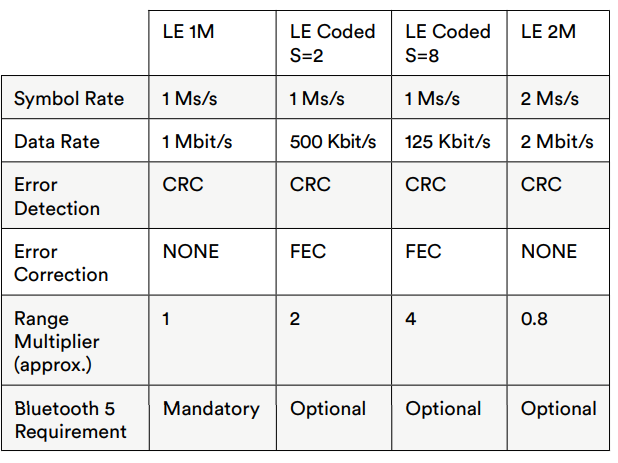
\includegraphics[width=0.8\textwidth]{./images/LE_PHY_edited.png}
		\caption{Comparació de diferents capes físiques \cite{BLE_5_improvement_over_4}}
		\label{FEC}
	\end{center}
\end{table}

\subsubsection{Advertisement Extensions}
\label{Advertisement_Extensions}
En Bluetooth 4.0 els paquets d'anunci (\textit{Advertisement Packets}) tenen 6 octets de capçalera i com a molt 31 de dades, és a dir, com a molt es poden transmetre 31 Bytes de cop.
Normalment, aquests paquets es transmeten pels 3 canals d'anunci el 37, 38 i 39.

En Bluetooth 5 per poder difondre (\textit{broadcast}) més dades el que es fa és enviar un paquet d'anunci on només s'indica la capçalera i un punter cap al canal per on s'enviarà el paquet complet.
Posteriorment, pel canal per on s'ha indicat s'envia el paquet de dades i en cas de necessitar més dades s'encadenen paquets.
D'aquesta manera, les dades només es transmeten una vegada, no com en la versió 4, on calia transmetre-les en els tres canals d'anunci.
Aquest procediment està detallat més endavant en l'apartat  \ref{Advertising_Extension_PDU}

En la versió 4.0 quan es vol enviar un paquet és necessari esperar un cert temps aleatori.
Aquest procediment evita les col·lisions periòdiques però suposa que els dispositius han d'estar durant més temps escoltant, ja que no saben quan rebran el paquet exactament.
En BLE 5 el GAP, que s'explicarà en profunditat a l'apartat \ref{GAP}, defineix un mode síncron que permet utilitzar un procediment d'establiment d'anunciaments sincronitzats.
Per poder-ho fer existeix una nova capçalera \textit{SyncInfo} on s'indica amb exactitud l'interval i variació dels paquets.
Així doncs, s'aconsegueix evitar les col·lisions i alhora reduir el temps que el dispositiu ha de tenir la ràdio encesa.

\subsubsection{Slot Availability Masks}
La tecnologia LTE (telefonia) està utilitzant cada vegada més espai freqüencial i en preparació que s'utilitzi en freqüencials pròximes a la banda de 2,4 GHz ISM s'ha desenvolupat un sistema per indicar disponibilitat en el temps dels diferents canals.
Per evitar les possibles interferències que causin altres tecnologies, es defineix la SAM (\textit{Slot Availability Mask}) que permet identificar aquelles ranures de temps on hi ha disponibilitat així bloquejant aquells moments on hi hagi interferències per evitar-les.

\subsubsection{Improved Frequency Hopping}
Els salts en freqüència que utilitza la versió 4.0 estan definits per 12 seqüències predeterminades.
En canvi, BLE 5 utilitza una seqüència pseudoaleatòria per determinar quins canals s'utilitzen.
L'algorisme, en aquest cas, és el \textit{channel selection algorithm \#2} i és més efectiu a evitar interferències i esvaniments per propagació multicamí.
Aquesta tècnica de modulació s'explicarà en més detall a l'apartat \ref{link_layer}

\section{Pila BLE}
Un cop vistes les característiques generals del protocol cal entendre com funciona per dins.
A continuació, es descriurà la pila de BLE i es veurà cada una de les capes que en formen part i les seves funcions.

\begin{figure}[h!]
	\begin{center}
		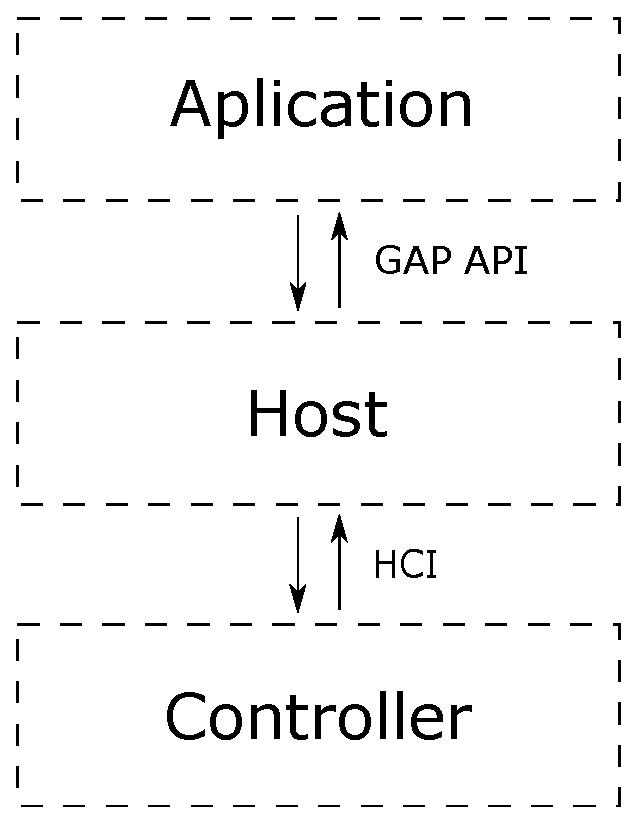
\includegraphics[width=0.4\textwidth]{./diagrames/BLE_Stack_Simplified}
		\caption{Pila de BLE}
		\label{ble_stack}
	\end{center}
\end{figure}

La pròpia pila de Bluetooth Low Energy està dividida en dues parts, el controlador i el \textit{host}.
Tal com es pot observar a la Figura \ref{ble_stack} són dues parts independents i utilitzen el protocol \textit{Host Controller Interface} (HCI d'ara endavant) per comunicar-se entre elles.
Aquest protocol pot estar implementat amb qualsevol protocol de transport físic com USB o UART.
La idea de separar la pila en dos és per fer compatibles xips fets per diferents fabricants.
Les dues parts de la pila poden ser implementades en el mateix xip anomenat configuració única o en xips separats anomenat configuració dual.


\subsection{Controller}
El controlador compren la capa física i la capa d'enllaç en l'ordre que mostra la Figura \ref{controller_stack}.

\begin{figure}[h!]
	\begin{center}
		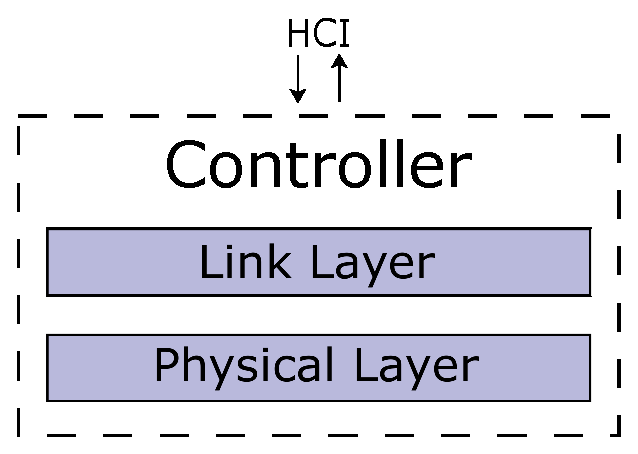
\includegraphics[width=0.5\textwidth]{./diagrames/BLE_Controller}
		\caption{Controller Stack}
		\label{controller_stack}
	\end{center}
\end{figure}

Per sota del controlador hi hauria l'antena que transmetria i rebria els senyals.

\subsubsection{Capa Física}
La capa física és la que s'encarrega de la comunicació anal·lògica modulant i desmodulant els senyals.
Tal i com ja s'ha comentat abans, treballa a la banda de 2,4 GHz en 40 canals diferents tal i com es mostra a la Figura \ref{BLE_Channels}.

\begin{figure}[hb]
	\begin{center}
		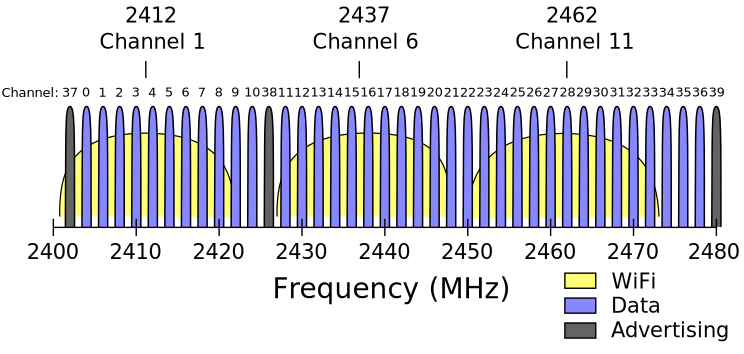
\includegraphics[width=0.8\textwidth]{./diagrames/BLE_WiFi}
		\caption{Canals BLE \cite{ble_feq}}
		\label{BLE_Channels}
	\end{center}
\end{figure}

Els canals es classifiquen en 37 de dades o també anomenats secundaris i 3 d'anunci (\textit{Advertisment}) o primaris.
En els canals d'anunci es vol tenir més qualitat, ja que la informació que s'hi transmet és més important.
Per exemple, són els canals que s'utilitzen per descobrir altres dispositius.
És per això, que els canals d'anunci es troben en el buits que deixen els canals WiFi més comuns (1, 6 i 11), tal com es veu a la Figura \ref{BLE_Channels}.

El protocol BLE té l'objectiu de consumir el mínim d'energia possible, això es pot millorar reduint el temps que s'està transmetent o escoltant a través de la ràdio.
Si no s'ha de rebre o transmetre res, es pot apagar la ràdio i s'estalvia energia.
El BLE és un dels protocols que tenen la taxa de transmissió física \footnote{La taxa de transmissió física és aquella a la que transmeten la ràdio, no confondre amb la taxa de dades d'aplicació \textit{Throughput}} més alta d'entre les MANETs, i de fins a 1 Mbps originalment i de 2 Mbps en BLE 5.

La potència màxima de transmissió és de 20 dBm (100 mW) segons l'especificació\footnote{La PCB utilitzada pot transmetre fins a 5 dBm de potència}.
Aquesta potència de la ràdio es pot controlar, disminuint-la per consumir menys energia.
Tot i que això, només serà possible si l'entorn ho permet i el receptor pot rebre el senyal correctament.
Els paquets de BLE indiquen la potència amb que s'han transmès i junt amb el RSSI (\textit{Received Signal Strength Indicator}), la potència rebuda, es pot estimar la distància fins al transmissor.
Conèixer aquest valor és útil per a certes aplicacions, per exemple, la localització en espais interiors.

La modulació utilitzada per BLE és la GFSK (\textit{Gaussian Frequency Shift Keying}), aquesta modulació és una de les més robustes, simples d'implementar i és el que permet a BLE, en part, tenir un abast molt més gran que Bluetooth Clàssic.
El filtre gaussià redueix el pic de consum d'energia \cite{BLE_Review} i també redueix les interferències en freqüències veïnes.
En BLE 4.0 s'utilitza una desviació freqüencial de 185 kHz, en BLE 5 com que augmenta la velocitat de símbols també la necessitat de protegir-se de la interferència intersimbòlica.
Per mitigar aquest efecte negatiu, la desviació de freqüència passa a ser de 370 kHz.


\subsubsection{Link Layer}
\label{link_layer}
La capa d'enllaç és l'encarregada d'escanejar, anunciar i gestionar les connexions amb altres dispositius.

\begin{figure}[!h]
	\begin{center}
		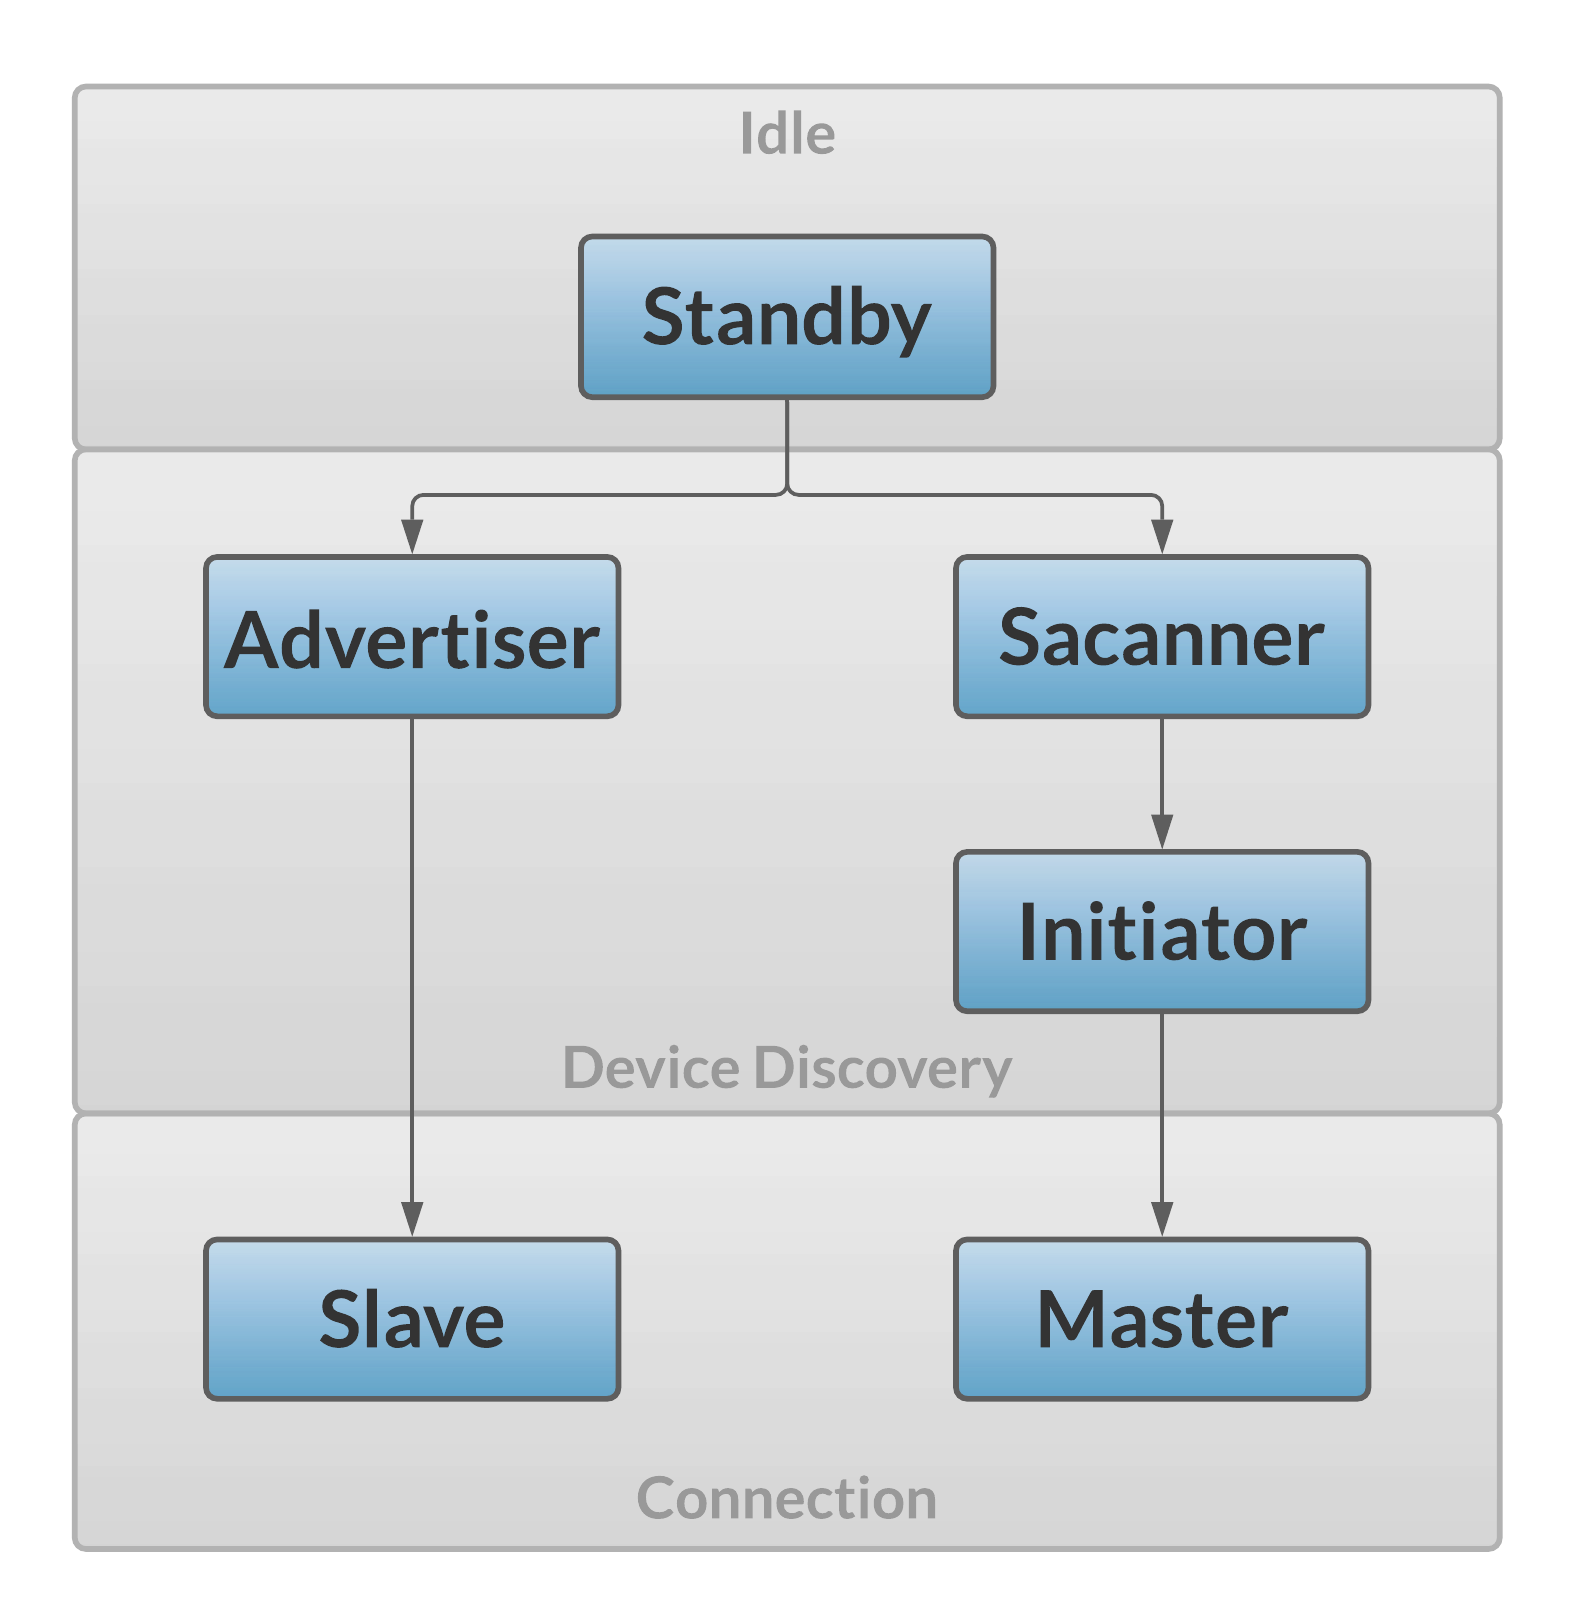
\includegraphics[width=0.6\textwidth]{./images/link_state_diagram.png}
		\caption{Estats de la capa d'enllaç \cite{Link_Layer_states}}
		\label{Link_State_Diagram}
	\end{center}
\end{figure}

Depenent del moment en la connexió, els dispositius es troben en diferents estats.
Els estats son: Espera (\textit{Standby}), Anunciador (\textit{Advertiser}) o Escàner (\textit{Scanner}) i Iniciador (\textit{Initiator}), Esclau (\textit{Slave}) o Mestre (\textit{Master}).
A la Figura \ref{Link_State_Diagram} s'hi pot veure el diagrama d'estats per arribar a una connexió.

Aquesta capa és l'encarregada d'implementar el salt en freqüència (\textit{frequency hopping}) que permet mitigar l'impacte de les interferències estretes.
Si s'utilitzés només un dels canals BLE i en aquell canal hi haguessin interferències no es podria establir comunicació.
Al alternar múltiples canals, encara que hi hagi interferències en algun d'ells es considera probable que no n'hi haurà en tots i per tant hi podrà haver una bona comunicació.
Els salts que es fan són des de 5 fins 16 canals per salt d'entre els dedicats a dades.

\subsection{Host}
El protocol BLE es va dissenyar amb la flexibilitat en ment, és per això que l'estructura de la pila del host permet no utilitzar certes capes que es consideren opcionals tal com es pot veure a la Figura \ref{host_stack}.
El permetre tenir capes opcionals pot generar incompatibilitats entre dispositius però no és comú.
En canvi, facilita molt i abarateix el disseny d'un dispositiu BLE en cas que no es necessitin totes les capacitats que ofereix.

\begin{figure}[h!]
	\begin{center}
		
\includegraphics[width=0.8\textwidth]{./images/ble_host_stack.png}
		\caption{Pila del Host \cite{ble_stack}}
			\label{host_stack}
	\end{center}
\end{figure}

\subsubsection{L2CAP (\textit{Logical Link Control and Adaptation Protocol})}
La \textit{Logical Link Control and Adaptation Protocol} és la capa encarregada de l'establiment de la connexió lògica; segmentació i reassemblatge de paquets; multiplexament de protocols;  i control de flux individual per canal.

La multiplexació de protocols és necessària per aconseguir que BLE sigui flexible.
Permet que des de capes superiors s'utilitzin els protocols que necessiti el fabricant, i no només aquells determinats per l'estàndard de BLE.

Degut a la limitació física de l'arquitectura, existeix una MTU\footnote{La MTU és la mida màxima que pot tenir un paquet} (\textit{Maximum Transmission Unit}) i per tant és necessari segmentar els paquets de les capes superiors que es converteixen en paquets més petits per a les capes inferiors.
Aquesta MTU es pot definir (dins dels límits establerts) independentment per cada connexió així flexibilitzant l'ús que es dóna al protocol en cada cas.
La L2CAP també és la capa que fa el seguiment de la qualitat de la connexió i dels recursos utilitzats per assegurar-se que les necessitats dels serveis es compleixen.

\subsubsection{\textit{Security Manager}}
La capa \textit{Security Manager} o SM proveeix de diferents serveis relacionats amb la seguretat de la connexió.
Aquests serveis són: autenticació i autorització de dispositius; i també integritat, confidencialitat i privacitat de les dades.
El protocol té flexibilitat en el tipus d'emparellament i la generació de claus per aconseguir reduir els requeriments de memòria i energia segons les necessitats específiques.
Els diferents mètodes de seguretat es comentaran en més profunditat a l'apartat \ref{sec:security}

\subsubsection{ATT \& GATT}
L'\textit{Attribute Protocol} (ATT d'ara endavant) és el protocol d'aplicació més comú per a BLE i el \textit{Generic Attribute Profile} (GATT d'ara endavant) defineix com utilitzar el protocol per oferir serveis a capes superiors.
L'ATT és un protocol dissenyat per a dispositius \textit{Low Energy} amb l'objectiu de minimitzar la quantitat de dades transmeses.
El protocol defineix el concepte d'Atributs, que estan formats per 4 elements, el \textit{handle}, l'UUID, els permisos  i el \textit{value}.

El \textit{handle} fa la distinció única entre els diferents atributs, ocupa 16 bits i habitualment, però no obligatòriament, els valors són seqüencials. És molt útil, ja que s'utilitza per referenciar l'atribut amb el mínim de bits possibles.
L'UUID (\textit{Universal Unique IDentifier}) identifica el tipus d'atribut, aquest número pot ser de 16 bits si s'utilitza algun que ja està estandarditzat pel SIG o bé en tindrà 128 bits si està definit pel fabricant.
En els permisos s'indicarà quin tipus d'accés té el client a la informació que s'explicarà en profunditat a l'apartat \ref{sec:properties}
També pot estar definit si requereix un nivell mínim d'encriptació o si és necessari l'autenticació.
Finalment, el valor de l'atribut serà on hi ha la informació, la seva interpretació i longitud (512 bytes com a molt) que dependrà de l'UUID.

\begin{figure}[h!]
	\begin{center}
		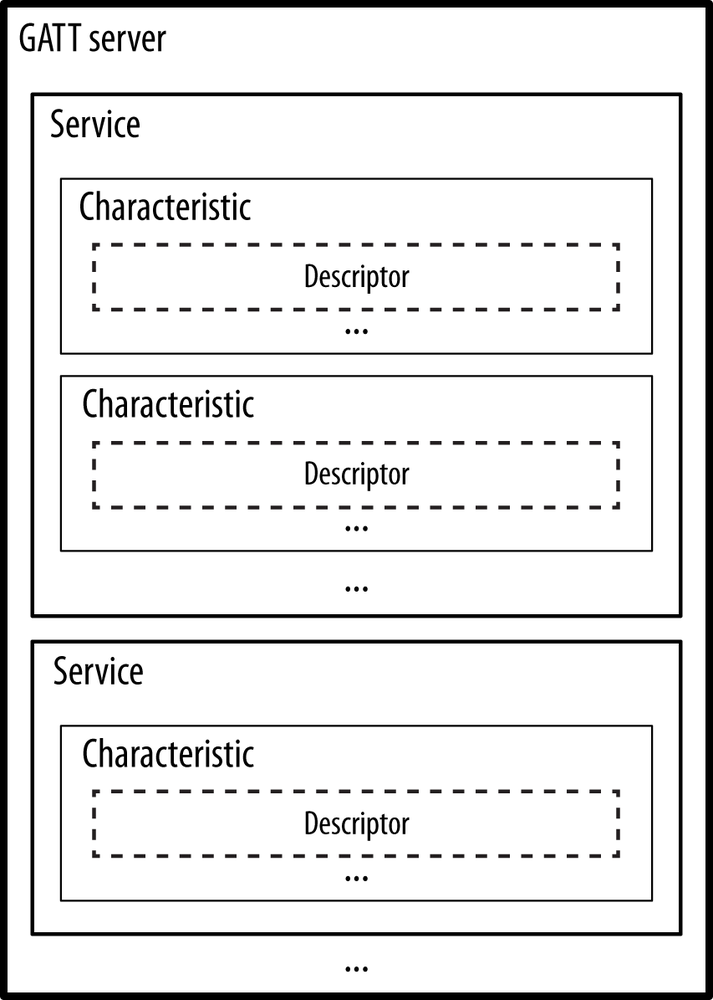
\includegraphics[width=0.4\textwidth]{./images/GATT_Hierarchy.png}
		\caption{Jerarquia de GATT \cite{GATT_Hierarchy}}
		\label{fig:Gatt_Hierarchy}
	\end{center}
\end{figure}

Des de la perspectiva del GATT els dispositius són clients i servidors.
Habitualment és el client qui pren la iniciativa demanant dades, tot i així, el servidor també té la capacitat d'iniciar una comunicació per exemple notificant quan un valor ha canviat.

La definició de l'ATT és massa genèrica per si sola tal que seria comú que, per fer el mateix, es desenvolupessin múltiples definicions que fossin incompatibles entre si.
Per tal de tenir millor definits els serveis s'utilitza el GATT.
El GATT permet definir perfils que agrupen múltiples atributs en un sol servei \cite{services}, la seva jerarquia es mostra en la Figura \ref{fig:Gatt_Hierarchy}.

En un llistat d'atributs el GATT identifica els serveis tenint en compte que cada servei comença amb un atribut amb l'UUID 0x2800.
Aquest atribut amb UUID 0x2800 s'anomena Declaració de Servei i tots els atributs consecutius fins a una altra declaració de servei formen part d'aquest.
En la declaració de servei el camp ``valor'' indica l'UUID que identifica de quin servei es tracta.
Cada servei conté característiques \cite{characteristics} definides en els atributs amb UUID 0x2803.
Aquests tipus d'atributs s'anomenen Declaració de Característica.
El valor de la declaració de característica està format per un nou UUID que identifica la característica i per un \textit{handle}.
Aquest \textit{handle} correspon a l'atribut on hi ha les dades de la característica.

\begin{table}[h]
	\begin{center}
		\definecolor{lightred}{RGB}{255, 128, 128}
		\definecolor{lightyellow}{RGB}{238, 232, 170}
		\begin{tabular}{|l|l|l|l|}
			\hline
			\textbf{Handle}	&	\textbf{UUID}	&	\textbf{Descripció}						&	\textbf{Valor}		\\ 	\hline \rowcolor{lightred}
			0x0100	&	0x2800	&	Battery Service					&	UUID 0x180F	\\		\hline \rowcolor{lightyellow}
			0x0101	&	0x2803	&	Characteristic: Battery Level	&	\parbox[t]{4cm}{UUID 0x2A19	\\ Value handle: 0x0102}	\\	\hline
			0x0102	&	0x2A2B	&	Battery Value					&	20	\\	\hline	\rowcolor{lightred}
			0x0103	&	0x2800	&	Custom Temperature Service		&	UUID 	706676c8-3e49...	\\	\hline	\rowcolor{lightyellow}
			0x0104	&	0x2803	&	Characteristic: Temperature		&	\parbox[t]{4cm}{UUID 0x2A6E	\\ Value handle: 0x0105}	\\		\hline	
			0x0105	&	0x2A6E	&	Temperature Value				&	25.45	\\	\hline \rowcolor{lightyellow}
			0x0106	&	0x2803	&	Characteristic: date/time		&	\parbox[t]{4cm}{UUID 0x2A08	\\ Value handle: 0x0107}	\\		\hline
			0x0107	&	0x2A08	&	Date/Time						&	1/1/1980 12:00	\\
			\hline
		\end{tabular}	
		\caption{Exemple de possibles atributs}
		\label{Attribute_Table}
	\end{center}
\end{table}

En aquest exemple de la Taula \ref{Attribute_Table} es pot observar que hi ha dos serveis diferents, marcats en vermell, ja que hi ha dos UUID 0x2800.
També es mostren tres declaracions de característiques en total, marcades en groc, (una pel primer servei i dues pel segon) que corresponen als tres atributs amb UUID 0x2803.
Com que els valors corresponents al nivell de bateria i la temperatura estan estandarditzats (veure \cite{Battery_Level}\cite{Temperature_Characteristic}, respectivament), no cal especificar que es refereixen a percentatge de bateria restant i a graus Celsius.

En canvi, la declaració de servei de temperatura (\textit{Handle} 0x0103) es pot veure que no forma part de l'estàndard, ja que el seu valor té 128 bits.
S'ha escollit per a aquest projecte un UUID completament aleatori, en concret el 706676c8-3e49-4ecc-9379-fa9851444e53.
Aquest UUID identifica el servei que s'ha desenvolupat per l'exemple i en teoria hauria de ser únic.
No es pot saber amb seguretat que algun altre desenvolupador no hagi escollit el mateix UUID i no hi ha una coordinació establerta.
Tot i això es considera del tot improbable que es produeixin col·lisions degut a la longitud de 128 bits.

La condició que ha de complir l'UUID és que no acabi en 0000-1000-8000-00805F9B34FB, ja que aquest sufix correspon als que estan reservats segons l'estàndard.
És possible demanar al SIG tenir un UUID global reservat per a ús propi amb un cost de \$2.500.
Es poden veure tots els que ja s'han reservat oficialment a \cite{reservedUUIDs}.

En aquest exemple no n'hi ha cap però les característiques poden tenir descriptors \cite{descriptors} que permeten aportar informació addicional sobre la característica que els precedeix.
Aquests, per exemple, serveixen per poder subscriure's a rebre notificacions cada cop que una característica canvia de valor.
Els atributs també tenen propietats d'accés que defineixen quines accions es poden prendre.
Les diferents propietats de l'estàndard es comentaran amb més detall en un exemple real més endavant \ref{sec:properties}

\subsubsection{GAP}
\label{GAP}
La \textit{Generic Access Profile} és la capa que interactua amb l'aplicació i per tant ofereix la Interfície de Programació d'Aplicacions (API en anglès) amb la funcionalitat que aporta BLE.

El dispositiu sempre està en un\footnote{Si s'utilitza el Mesh Profile, que s'explicarà més endavant és possible que un dispositiu tingui més d'un rol, però sempre en tindrà un únic rol per connexió.} dels quatre rols: Emissor, Observador, Perifèric o Central.
Si el rol és emissor, s'enviaran anuncis per poder ser descobert.
Si és Observador s'escoltaran els canals per obtenir informació dels anuncis.
Un cop s'estigui en una connexió el Perifèric serà el node amb menys capacitats de processament o de bateria i és requerirà menys d'ell per mantenir la connexió, per exemple a un rellotge intel·ligent
En canvi el node Central serà el que tingui més recursos com pot ser un telèfon intel·ligent o un ordinador.
Amb aquests rols i l'especificació del GAP existeix l'estàndard que permet els dispositius descobrir-se, connectar-se i emparellar-se entre d'altres.
\newpage


\section{Anunciaments}
Els paquets d'anunci com ja s'ha explicat anteriorment són aquells que serveixen a un dispositiu per donar-se a conèixer i alhora opcionalment transmetre informació \cite{Advertising}.
BLE és molt flexible a l'hora de configurar els paràmetres d'anunci i permet al desenvolupador adaptar el protocol per a les necessitats que tingui.
A continuació, es concretarà quins són aquests paràmetres i com afecten les prestacions finals del sistema.


\subsection{Tipus}
Existeixen 4 paquets d'aquest tipus i BLE 5 n'afegeix 4 més.
Els 4 originals es classifiquen segons si permet connexió i si permeten escaneig, tal com mostra la Taula \ref{tab:Advertisment_Types}.

\begin{table}[!h]
	\begin{center}
		\begin{tabular}{|c|c|l|}
			\hline
			Connexió	&	Escaneig	&	Nom	\\	\hline
			Si			&	Si			&	ADV\_IND	\\	\hline
			Si			&	No			&	ADV\_DIRECT\_IND	\\	\hline
			No			&	No			&	ADV\_NONCONN\_IND	\\	\hline
			No			&	Si			&	ADV\_SCAN\_IND	\\	\hline
		\end{tabular}
	\end{center}
\caption{Tipus d'anunciaments}
\label{tab:Advertisment_Types}
\end{table}


L'anunci ADV\_IND és el més comú i permet que qualsevol dispositiu pugui connectar-se.
L'ADV\_DIRECT\_IND serveix per anunciar-se a un dispositiu específic, per exemple, si un rellotge intel·ligent es vol connectar al telèfon al qual està associat.
L'ADV\_NONCONN\_IND només indica que existeix i no rebrà informació.
Això és útil, per exemple, per permetre localització de balises.
L'ADV\_SCAN\_IND també està orientat a balises però estarà escoltant per si rep missatges d'escaneig amb els que pot respondre amb poca informació.
Això permet una comunicació bidireccional limitada sense necessitat d'establir connexió.
Tots els paquets excepte l'ADV\_DIRECT\_IND permeten transmetre 31 bytes de dades pròpies que han de seguir el format establert que s'explicarà a l'apartat \ref{sec:format}

\label{Advertising_Extension_PDU}
En BLE 5 s'afegeixen 4 paquets més que permeten augmentar la quantitat de dades que es poden transmetre abans d'haver establert una connexió.
L'ADV\_EXT\_IND és el paquet que s'envia pels canals d'anunci i indica en quin canal secundari s'enviarà l'anunci. Aquest paquet no permet transmetre dades.
Els paquets que s'envien per canals secundaris tenen el prefix ``AUX'' i permeten enviar fins a 255 bytes de dades pròpies.
L'AUX\_ADV\_IND és el paquet que s'envia per un canal secundari després que s'hagi indicat pel tipus de paquet anterior.
En aquest paquet es pot configurar si es permet o no connexió i escaneig però no les dues.
L'AUX\_SYNC\_IND s'utilitza per indicar que s'enviaran anuncis periòdics pels canals secundaris.
D'aquesta manera no cal utilitzar els canals d'anunci tan sovint.

Si es vol transmetre tanta informació com es vulgui sense necessitat d'establir una connexió es pot fer amb la seqüència de paquets tal com mostra la Figura \ref{fig:aux_chain_ind}.
En primer lloc, l'anunciador envia pels canals d'anunci (habitualment s'envia múltiples vegades per cada canal primari) l'ADV\_EXT\_IND.
Posteriorment, es transmet pel canal secundari l'AUX\_ADV\_IND que indica quan i on es transmetrà el següent paquet.
Finalment, es transmeten tants AUX\_CHAIN\_IND com siguin necessaris fins que s'hagi enviat totes les dades d'anunci que es vulgui.

\begin{figure}[h!]
	\begin{center}
		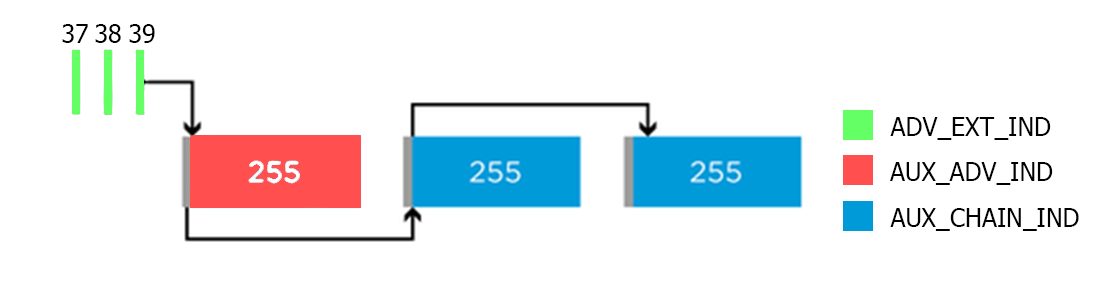
\includegraphics[width=1\textwidth]{./images/aux_chain_ind.png}
		\caption{Exemple d'anunci estès \cite{adv_ext}}
		\label{fig:aux_chain_ind}
	\end{center}
\end{figure}



\subsection{Paràmetres}
BLE permet seleccionar qualsevol combinació de canals primaris per on transmetre els anuncis.
Per consumir menys energia es pot transmetre en un únic canal però això es recomana no fer-ho, ja que si el canal és sorollós, els dispositius no el podran detectar.

Un paràmetre molt important que es pot configurar és l'interval d'anunci (\textit{Advertising Interval}, en anglès).
Aquest valor defineix el temps que passa entre que es transmeten anuncis pel mateix canal tal com es pot veure en la Figura \ref{fig:advertisment_params}.
L'especificació de BLE defineix que pot estar entre 20 ms i 10,24 s amb salts de 0,625 ms.
Aquest paràmetre és crític depenent del servei que es vol oferir.
Si el valor és molt alt, ajudarà a reduir el consum d'energia considerablement, però això augmentarà la latència de descobriment de dispositius.
En canvi, si és molt baix, es reduirà la latència, però augmentarà molt el consum del dispositiu.

\begin{figure}[h!]
	\begin{center}
		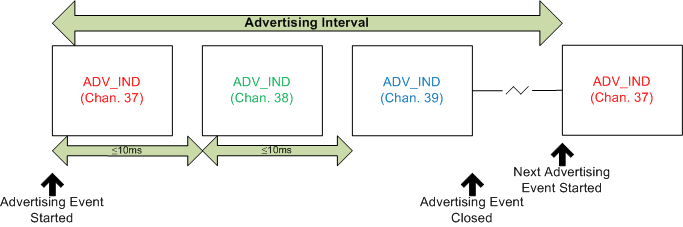
\includegraphics{./images/advertisement_params.png}
		\caption{Paràmetres d'anunci \cite{advertisment_params}}
		\label{fig:advertisment_params}
	\end{center}
\end{figure}


Un cop s'estableix la connexió ja es poden enviar dades ràpidament, però per l'escaneig són necessaris múltiples intervals d'anunci i cal considerar que és possible que el receptor no detecti tots els anuncis. 
És per això que, quan es desenvolupen serveis que interaccionen amb persones no és acceptable haver d'esperar desenes de segons, per tant, habitualment s'utilitzen valors d'entre 100 i 500 ms.
En canvi, per a dispositiu que requereixen la mínima latència possible en les dades s'utilitzen valors entre 20 i 50 ms.
Finalment, aquells dispositius que proporcionen dades que no varien sovint i que no requereixen interacció utilitzen valors des d'1 fins a 5 segons.

Al definir l'interval d'anunci cal tenir en compte que segons l'especificació de BLE (tal com s'ha comentat anteriorment a l'apartat \ref{Advertisement_Extensions}) s'aplica un retard pseudoaleatori que pot ser de fins a 10 ms i afecta els serveis que requereixen molt poca latència.
Aquest retard aleatori s'implementa per evitar col·lisions entre dispositius que s'han sincronitzat involuntàriament i tenen el mateix interval o un múltiple entre si.

Fins ara s'ha parlat de definir un únic valor d'interval d'anunci, però habitualment, s'estableix un règim on es va canviant aquest valor depenent de la situació.
Quan el dispositiu s'encén o quan s'espera una connexió es disminueix l'interval d'anunci per tal que la connexió s'estableixi més ràpidament.
En canvi, quan fa temps que no hi ha cap connexió s'augmenta l'interval d'anunci per reduir el consum d'energia i augmentar el temps de vida del dispositiu. 


\section{Escaneig}
Quan un dispositiu es vol donar a conèixer, a part de transmetre anuncis, també ho pot fer fent escaneigs a dispositius que s'han anunciat prèviament.
El procés d'escanejar en l'especificació de BLE 5 s'anomena \textit{Device Discovery} i es basa en dos tipus, l'escaneig actiu i el passiu.
En cas de fer escaneig passiu només es pot obtenir informació a través dels anuncis d'altres dispositius.
Si l'escaneig és actiu, es poden enviar requeriments d'escaneig per demanar informació addicional a la qual hi ha als anuncis.


\subsection{Tipus}
Per a l'escaneig actiu hi ha dos paquets en la versió 4.0 i BLE 5 n'afegeix dos més.
El requeriment d'escaneig SCAN\_REQ serveix per requerir més informació a un dispositiu que s'està anunciant i que accepta aquest tipus de petició.
En el paquet no hi van dades pròpies, només s'hi indica l'origen i destí.
L'SCAN\_RSP és la resposta al paquet anterior, conté l'adreça pròpia de l'anunciador i fins a 31 bytes de dades.
L'extensió que aporta BLE 5 defineix 2 nous tipus de paquets, l'AUX\_SCAN\_REQ i l'AUX\_SCAN\_RSP que tenen la mateixa funcionalitat que els anteriors respectivament.
La diferència és que serveixen per a les comunicacions a través de canals secundaris.
Conseqüentment la quantitat de dades passa a ser de fins a 254 bytes en la resposta.

\subsection{Paràmetres}
Els paràmetres d'escaneig són tan importants com els d'anunci, ja que també afecten considerablement al temps de vida del dispositiu.
Aquests paràmetres es poden identificar en la Figura \ref{fig:escaneig_canals}.

\begin{figure}[!h]
	\begin{center}
		\begin{subfigmatrix}{1}
			\subfigure[Escaneig de canals]{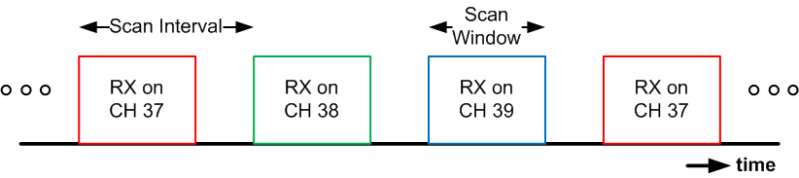
\includegraphics[width=0.9\textwidth]{./images/scanning_diagram}}
			\subfigure[Periodes d'escaneig]{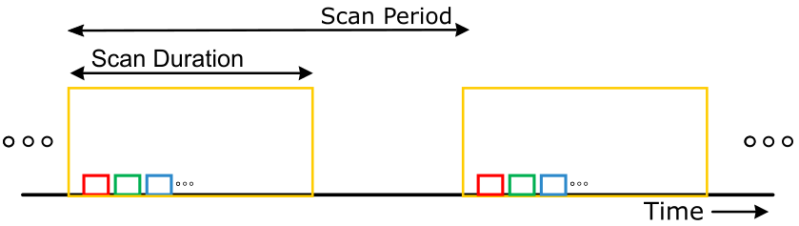
\includegraphics[width=0.9\textwidth]{./images/scanduationperiod}}
		\end{subfigmatrix}
	\end{center}
	\caption{Paràmetres d'escaneig \cite{advertisment_params} }
	\label{fig:escaneig_canals}
\end{figure}

L'interval d'escaneig o \textit{scan interval} és el temps des que es comença a escanejar en dos canals consecutius, es pot definir entre 10 ms i 10,24 s.
D'altra banda, la finestra d'escaneig o \textit{scan window} és el temps en què s'està escoltant a un canal.
Altrament ,la duració d'escaneig o \textit{scan duration}, és el temps que el dispositiu estarà escanejant.
Es pot configurar des de 10 ms fins a 65 segons o escaneig indefinit.
Finalment, el període d'escaneig o \textit{scan period} indica el temps entre que comencen les duracions d'escaneig i que serveix per poder fer pauses en què el dispositiu no escaneja.


\section{Connexions}
S'ha vist com, en BLE, no cal establir una connexió per a transmetre poca informació.
Això permet desenvolupar implementacions molt simples per a situacions on es transmet amb molt poca freqüència, com és el cas en xarxes de sensors.
Tot i això, BLE també permet transmetre moltes més dades quan s'estableix una connexió.

Un cop s'hagi establert la connexió es podrà transmetre la informació molt eficientment, però establir una connexió suposa un cost energètic significatiu en nodes low energy.
Per tant, a l'hora de definir els paràmetres de la connexió és important evitar, a ser possible, establir connexió cada vegada que es vol transmetre informació.

Com que les connexions estan basades en múltiples esdeveniments en instants determinats es considerà una connexió síncrona.
No hi ha límit de connexions segons l'especificació de BLE i per tant, dependrà de les capacitats del dispositiu amb el qual es treballa.


El dispositiu central serà el que iniciarà la connexió i el perifèric el que l'acceptarà o no.
El central serà sempre el mestre i el perifèric serà l'esclau de la connexió.
Per iniciar una connexió el mestre envia un missatge de tipus CONNECT\_IND\footnote{Aquest paquet en la versió 4 de BLE s'anomena CONNECT\_REQ} amb els paràmetres de la connexió.
En aquests paràmetres, tal com es veurà més endavant en l'apartat \ref{sec:params}, hi ha la informació necessària per determinar el primer esdeveniment de la connexió.
En cada esdeveniment, els dos dispositius tenen un temps assignat per transmetre i per rebre dades.

\begin{figure}[!h]
	\begin{center}
		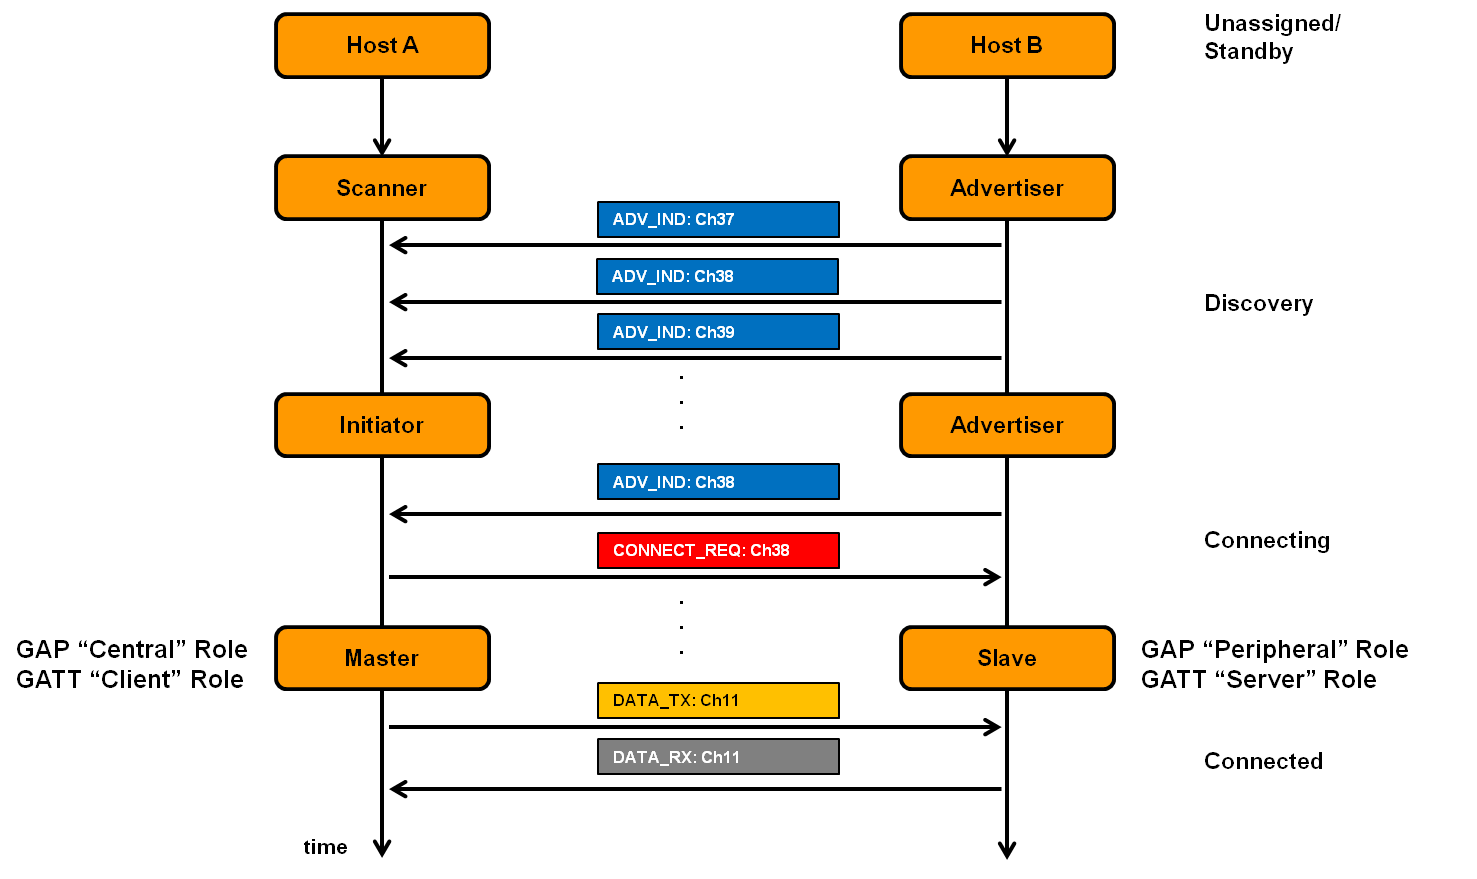
\includegraphics[width=1\textwidth]{./images/rols_unicast.png}
		\caption{Establiment de connexió \cite{fig:connection_establishement}}
		\label{fig:unicast_roles}
	\end{center}
\end{figure}


A la Figura \ref{fig:unicast_roles} es pot observar el procediment on els dos dispositius estableixen una connexió.
Tenim el dispositiu A que, inicialment, està com a observador i el dispositiu B que s'està anunciant.
Cal recordar que, no es detecten tots els anuncis, ja que els dispositius no sempre estan transmetent i escoltant en el mateix canal.
Per tant, serà necessari anunciar-se múltiples vegades en cada canal per assegurar-se que es rep l'anunci.

El dispositiu A rep un anunci de B, decideix establir una connexió i enviant un requeriment de connexió.
El dispositiu B després de transmetre un anunci per un canal, escolta durant un temps determinat en el mateix canal a l'espera de requeriments de connexió.
Quan el dispositiu B rep el requeriment, decideix acceptar la connexió i respon a aquest.

En aquest moment, el dispositiu A passa a ser el mestre amb els rols Central i Client i el dispositiu B passa a ser l'esclau amb rols de perifèric i servidor.
La connexió està establerta i ja és possible transmetre dades entre ambdós dispositius durant els esdeveniments de connexió. 


\subsection{Paràmetres}
\label{sec:params}
L'interval de connexió és un dels paràmetres més importants en la connexió BLE, estableix com de sovint es comuniquen els dispositius.
És el temps que hi ha entre esdeveniments de la connexió i va entre 7,5 ms i 4 s.
Com que el que es configuren són preferències, es determina l'interval mínim i el màxim que es vol.
En cas que es vulgui fixar, simplement, s'ha d'indicar el mateix valor per al mínim i al màxim.

BLE permet a l'esclau saltar-se esdeveniments per tal d'estalviar bateria, per exemple, si no té dades a transmetre.
La latència de l'esclau, que és un dels paràmetres de connexió, defineix la quantitat màxima d'esdeveniments que l'esclau es pot saltar sense que la connexió es perdi.

En la Figura \ref{fig:slave_latency} es pot observar la comparació entre utilitzar la latència d'esclau i no utilitzar-la.
Tot i això, el mestre que és el node que té més bateria, sempre participa en tots els esdeveniments escoltant el canal per si l'esclau transmet.
Utilitzar aquest paràmetre permet tenir una connexió amb una latència baixa, però amb un consum igualment reduït en el cas en que no s'hagin de transmetre dades molt sovint.

\begin{figure}[!h]
	\begin{center}
		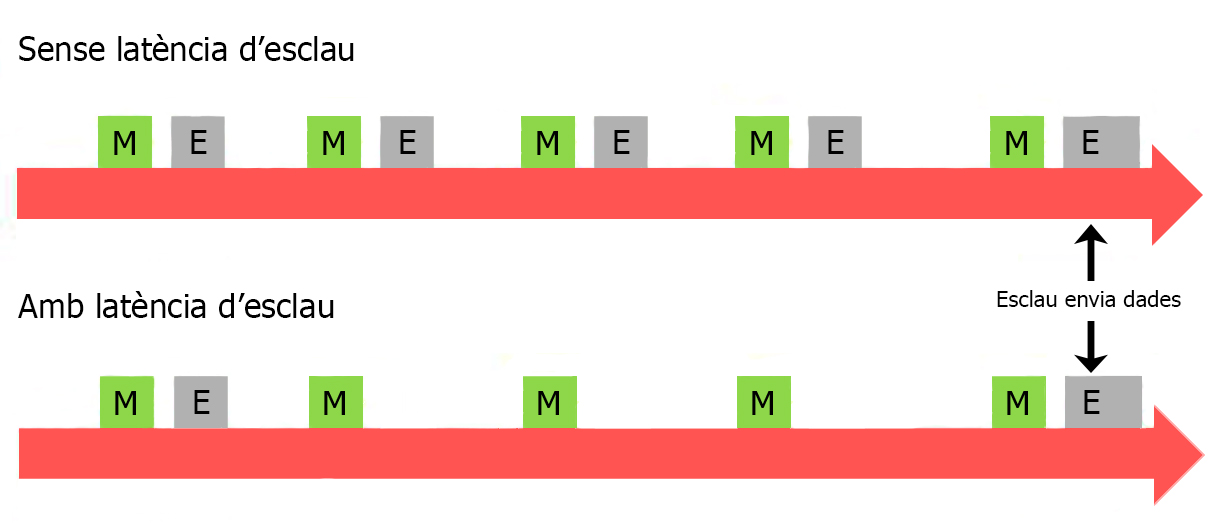
\includegraphics{./images/slave_latency_new.jpeg}
		\caption{Comparació d'esdeveniments amb latència d'esclau \cite{slave_latency}}
		\label{fig:slave_latency}
	\end{center}
\end{figure}

L'últim paràmetre rellevant és el temps de supervisió, és el temps màxim acceptable que pot passar sense activitat en la connexió.
Si es supera aquest temps, es considera que la connexió s'ha acabat i per tant, per comunicar-se s'ha de tornar a iniciar.
Això pot passar, per exemple, en entorns molt sorollosos o més sovint quan els dispositius surten del seu abast i el senyal no és detectable.

\section{Seguretat}
\label{sec:security}
Com que l'ús de BLE és molt flexible, per poder-lo utilitzar en certes aplicacions es requereix que l'intercanvi de dades sigui segur.
Això significa que la connexió tingui resistència a atacs d'\textit{eavesdrop}\footnote{Aquest tipus d'atac permet a l'atacant conèixer el contingut dels missatges que es transmeten.} passiu i d'intermediari\footnote{Aquest tipus d'atac permet modificar la informació que es transmet sense que sigui evident pel transmissor o el receptor.} (\textit{Man In The Middle} en anglès).
BLE utilitza l'encriptació simètrica AES-CCM, però la seguretat rau en com els nodes s'intercanvien la clau utilitzada per encriptar.

Es defineixen diferents sistemes per l'intercanvi de claus que el desenvolupador pot escollir i que varien en seguretat i facilitat d'ús.
Existeix el mètode sense seguretat anomenat \textit{Just Works}.
Aquest mètode és útil en casos on no es requereix seguretat o que no és possible tenir-ne per les limitacions del dispositiu amb el qual es vol establir connexió.

Un altre mètode és l'\textit{Out of Band}, aquest permet utilitzar una altra tecnologia per l'intercanvi de claus, com per exemple, NFC (comú en auriculars d'alta gamma).
La seguretat d'aquest mètode depèn completament en el nou sistema per l'intercanvi de claus.

El més habitual és el \textit{Passkey} en què l'intercanvi de claus es bassa en una contrasenya de 4 a 6 dígits.
Cal tenir en compte que, a causa del baix nombre de combinacions depenent de la implementació aquest mètode serà sensible a atacs d'\textit{eavesdropping} passiu.

Finalment, un mètode similar l'anterior és el de Comparació Numèrica, en lloc de ser l'usuari qui introdueix el codi es genera automàticament i es mostra en els dos dispositius.
Cal comprovar que sigui el mateix número en els dos casos i això permet prevenir atacs de \textit{Man in the Middle} però, de nou, no protegeix contra l'\textit{eavesdropping}.


\section{Format}
\label{sec:format}
En aquest apartat s'explicarà com estan formats els paquets que s'envien en BLE i de quins camps estan formats.
Cal distingir però entre la versió 4.2 i la 5 de BLE, ja que degut a les noves funcionalitats, el format canvia considerablement.

\subsection{BLE 4.2}
En la versió de BLE 4.2\footnote{En les versions anteriors a la 4.2 la PDU tenia una mida màxima de 39 bytes.} els paquets segueixen el format de la Figura \ref{fig:4_2_format}.

\begin{figure}[!h]
	\begin{center}
		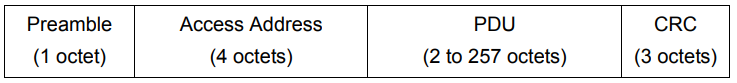
\includegraphics[width=1\textwidth]{./images/Packet_format_4_2.png}
		\caption{Format del paquet en BLE 4.2 \cite{BLE_4.2_packet_format}}
		\label{fig:4_2_format}
	\end{center}
\end{figure}

El preàmbul és una seqüència predefinida i que serveix per facilitar el sincronisme.
L'adreça d'accés identifica a quina connexió pertany aquest paquet, en cas de ser d'anunci i no pertànyer a cap connexió el valor és 0x8E89BED6.
Aquest camp serveix al receptor per filtrar els paquets i només tractar aquells que el poden interessar.
El CRC (Cyclic Redundancy Check) s'utilitza per detectar errors en el paquet. 

\begin{figure}[!h]
	\begin{center}
		\begin{subfigmatrix}{1}
			\subfigure[Format PDU d'anunci \cite{BLE_4.2_packet_format}]{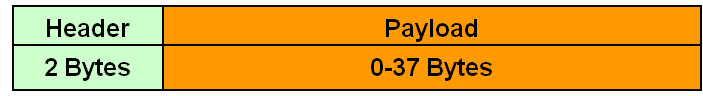
\includegraphics[width=0.8\textwidth]{./images/Packet_format_4_2_adv.png}}
			\subfigure[Format PDU de dades \cite{BLE_4.2_packet_format}]{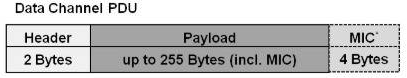
\includegraphics[width=0.8\textwidth]{./images/Packet_format_4_2_data.png}}
		\end{subfigmatrix}
	\end{center}
	\caption{Format PDU}
	\label{fig:pdu_format}
\end{figure}

En la PDU (Protocol Data Unit) és on es troba la informació pròpia del paquet i depenent de si és un paquet en un canal d'anunci o en un de dades té un format lleugerament diferent.
En la Figura \ref{fig:pdu_format} es poden veure les diferències.
Cal destacar que, en el cas de ser un anunci tot l'espai es dedica a informació, en canvi, en la PDU de dades es reserven 4 bytes per al comprovant d'integritat del missatge (\textit{Message Integrity Check} en anglès).

\begin{figure}[!h]
	\begin{center}
		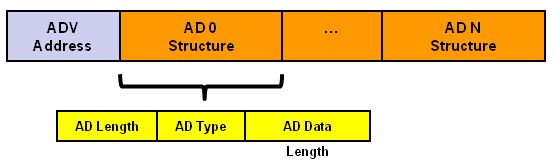
\includegraphics[width=0.8\textwidth]{./images/adv-ind-packet.png}
		\caption{Payload de ADV\_IND \cite{BLE_4.2_packet_format}}
	\end{center}
\end{figure}

Pel que fa a la Càrrega Útil o \textit{Payload} serà diferent segons el tipus de paquet.
En el cas de l'ADV\_IND està format per l'adreça de l'anunciant seguit d'un llistat d'estructures de dades d'anunci (\textit{Advertisement Data Structure}).
Aquestes, estan formades per la longitud de l'estructura, el tipus i les dades en si.
Existeixen molts tipus d'estructura que estan definits en l'estàndard \cite{AD_Types}.

En canvi, en el cas de l'ADV\_DIRECT\_IND simplement s'indica l'adreça de l'anunciador i la del dispositiu al qual va dirigit el paquet.

\subsection{BLE 5}
Els canvis per a BLE 5 corresponen a les noves possibilitats que s'han comentat a l'apartat \ref{Versions_BLE}
Principalment, la funcionalitat per poder transmetre anuncis als canals secundaris que s'ha comentat a \ref{Advertisement_Extensions} i enumerat els tipus de paquets a \ref{Advertising_Extension_PDU}

\begin{figure}[!h]
	\begin{center}
		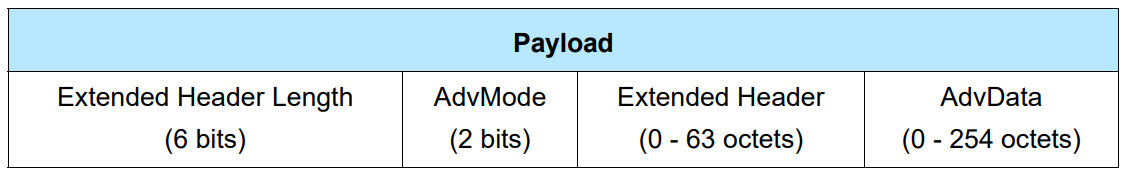
\includegraphics[width=0.9\textwidth]{./images/Common_Extended_Advertising_Payload_Format.png}
		\caption{Format de la Extended Advertising Payload \cite{BLE_5_Extended_Advertising}}
	\end{center}
\end{figure}

Tots els nous paquets d'anunci de BLE 5 es basen en aquest format flexible.
L'\textit{Extended Header Length} defineix la longitud del camp \textit{Extended Header}.
L'\textit{AdvMode} defineix una sèrie de valors que identifiquen si l'anunciador accepta connexions o es pot escanejar.
L'\textit{Extended Header} indica informació similar a la versió 4.2 com l'adreça de l'anunciador.
Però també indica tot el necessari per BLE 5, com en quin canal secundari es transmetrà part de la informació del paquet o amb quin tipus de capa física es transmetrà aquesta informació (LE 1M, LE 2M o LE Coded) entre d'altres.

\section{Xarxes Bluetooth multi-node}
Tal com s'ha vist fins ara, el Bluetooth Low Energy només permet tenir connectivitat punt a punt i això no és suficient per poder competir amb les altres tecnologies.
Si tenim un node que es connecta amb múltiples dispositius BLE, aquests no es poden comunicar entre si i això limita l'ús de BLE en grans desplegaments.
En canvi, les altres MANETs que s'han vist a l'apartat \ref{MANETS}; com Zigbee, 6LoWPAN o Z-Wave, entre d'altres, estableixen mecanismes que permeten connectar tots els nodes entre si a través d'una xarxa.

Bluetooth necessitava definir algun mètode oficial per poder implementar xarxes complexes entre nodes i ho va fer amb el \textit{Mesh Profile}.
El juliol del 2017 es va adoptar l'estàndard del perfil de malla (\textit{Mesh Profile} en anglès) format per la definició del perfil \cite{Mesh Profile Definition} i per la definició del models \cite{Mesh Profile Models}.

Aquest estàndard és molt rellevant per a BLE, ja que anteriorment no hi havia cap manera d'incrementar indefinidament l'abast.
En canvi, amb l'ús del \textit{Mesh Profile} és possible estendre la connectivitat amb nodes intermedis que facin de repetidors.
Però aquest no és l'únic avantatge que aporta, a continuació es descriurà resumidament com funciona el \textit{Mesh Profile} i com ajuda a augmentar les capacitats de BLE.

\subsection{Topologia}
Bluetooth té definicions per a diferents tipologies de nodes que es poden observar a la Figura \ref{piconet}.

\begin{figure}[!h]
	\begin{center}
		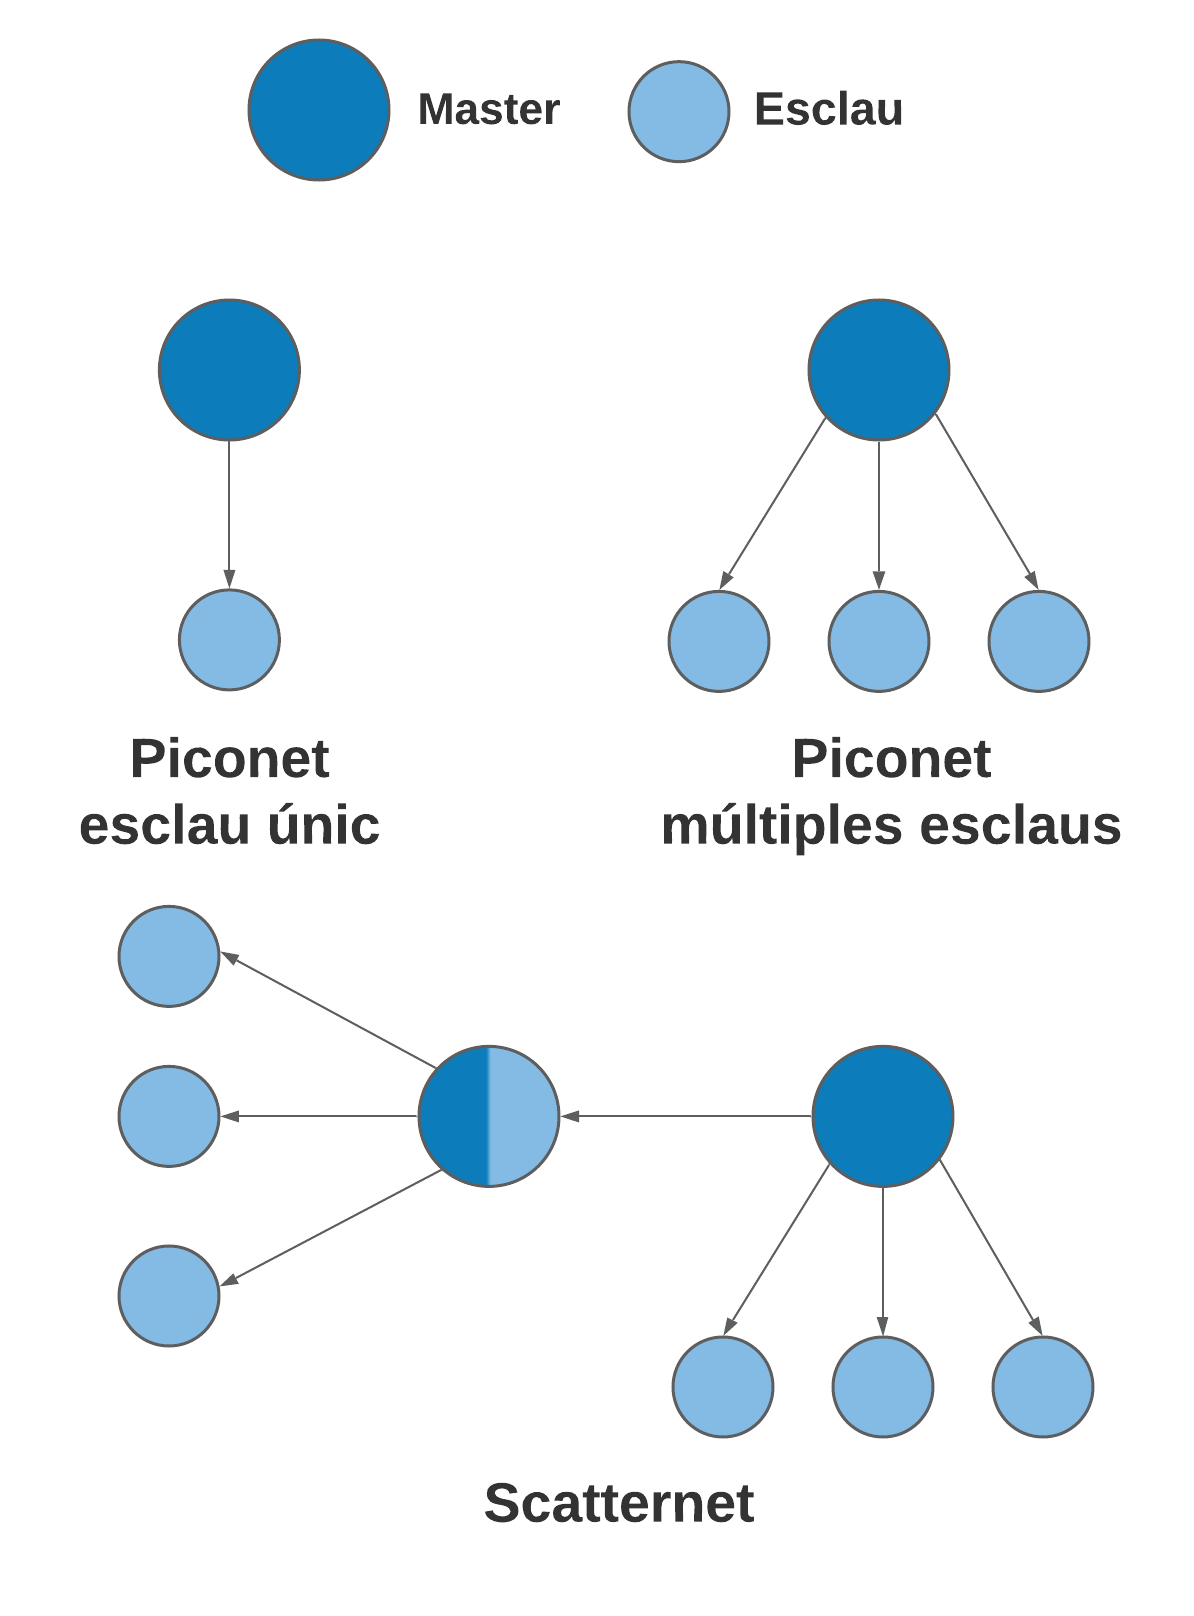
\includegraphics[width=0.52\textwidth]{./images/PICONET.png}
		\caption{Tipus de xarxes}
		\label{piconet}
	\end{center}
\end{figure}

En Bluetooth Clàssic els missatges que s'envien tenen un únic node origen i un únic node destí i per tant formen una \textit{Piconet} d'esclau únic.
Amb la introducció de BLE sorgeix la possibilitat d'enviar un mateix missatge amb potencialment múltiples dispositius com a destí, per exemple, utilitzant missatges d'anunci.
Aquestes d'interaccions són punt a multipunt, és a dir, un mestre pot estar connectat a més d'un esclau, però un esclau només estarà connectat a un mestre.
Aquest tipus de xarxa s'anomena \textit{Piconet} d'esclaus múltiples.

Gràcies al nou \textit{Mesh Profile} un node pot ser mestre en una connexió i esclau en una altra.
D'aquesta manera els nodes formen connexions multipunt a multipunt, és a dir, un mateix node pot estar connectat amb esclaus i mestres a la vegada.
Aquesta tipologia de xarxa està formada per múltiples \textit{piconets} interconnectades i en conjunt s'anomena \textit{scatternet}.

Pel reenviament dels paquets en lloc d'utilitzar protocols d'encaminament basats en IP s'utilitza encaminament d’inundació gestionat (\textit{managed flood routing}, en anglès).
L'ús d'aquest protocol és per fer el més simple possible el desenvolupament de dispositius així com reduir el sobrecost en processament i memòria.

És molt comú que en un desplegament es vulguin canviar múltiples elements a la vegada com poden ser llums, temperatura del termòstat i persianes.
Per reduir la quantitat de missatges enviats es poden utilitzar escenes que permeten interactuar amb múltiples nodes a la vegada.
Aquestes escenes es poden activar a través d'un únic missatge o també es poden programar perquè s'activin automàticament a una certa hora.

Cal destacar que, tot i que probablement la majoria de xarxes que utilitzin el \textit{Mesh Profile} no seran molt grans, l'estàndard s'ha dimensionat per poder tenir xarxes extremadament grans, pensades per pàrquings de cotxes, control d'il·luminació en edificis d'oficines o sensors en caps de futbol entre d'altres.
Els límits són de 32.767 nodes per xarxa, fins a 4.096 subxarxes i 65.535 escenes, i vénen marcats per la longitud dels camps corresponents que són de 15, 12 i 16 bits respectivament.

\begin{figure}[!h]
	\begin{center}
		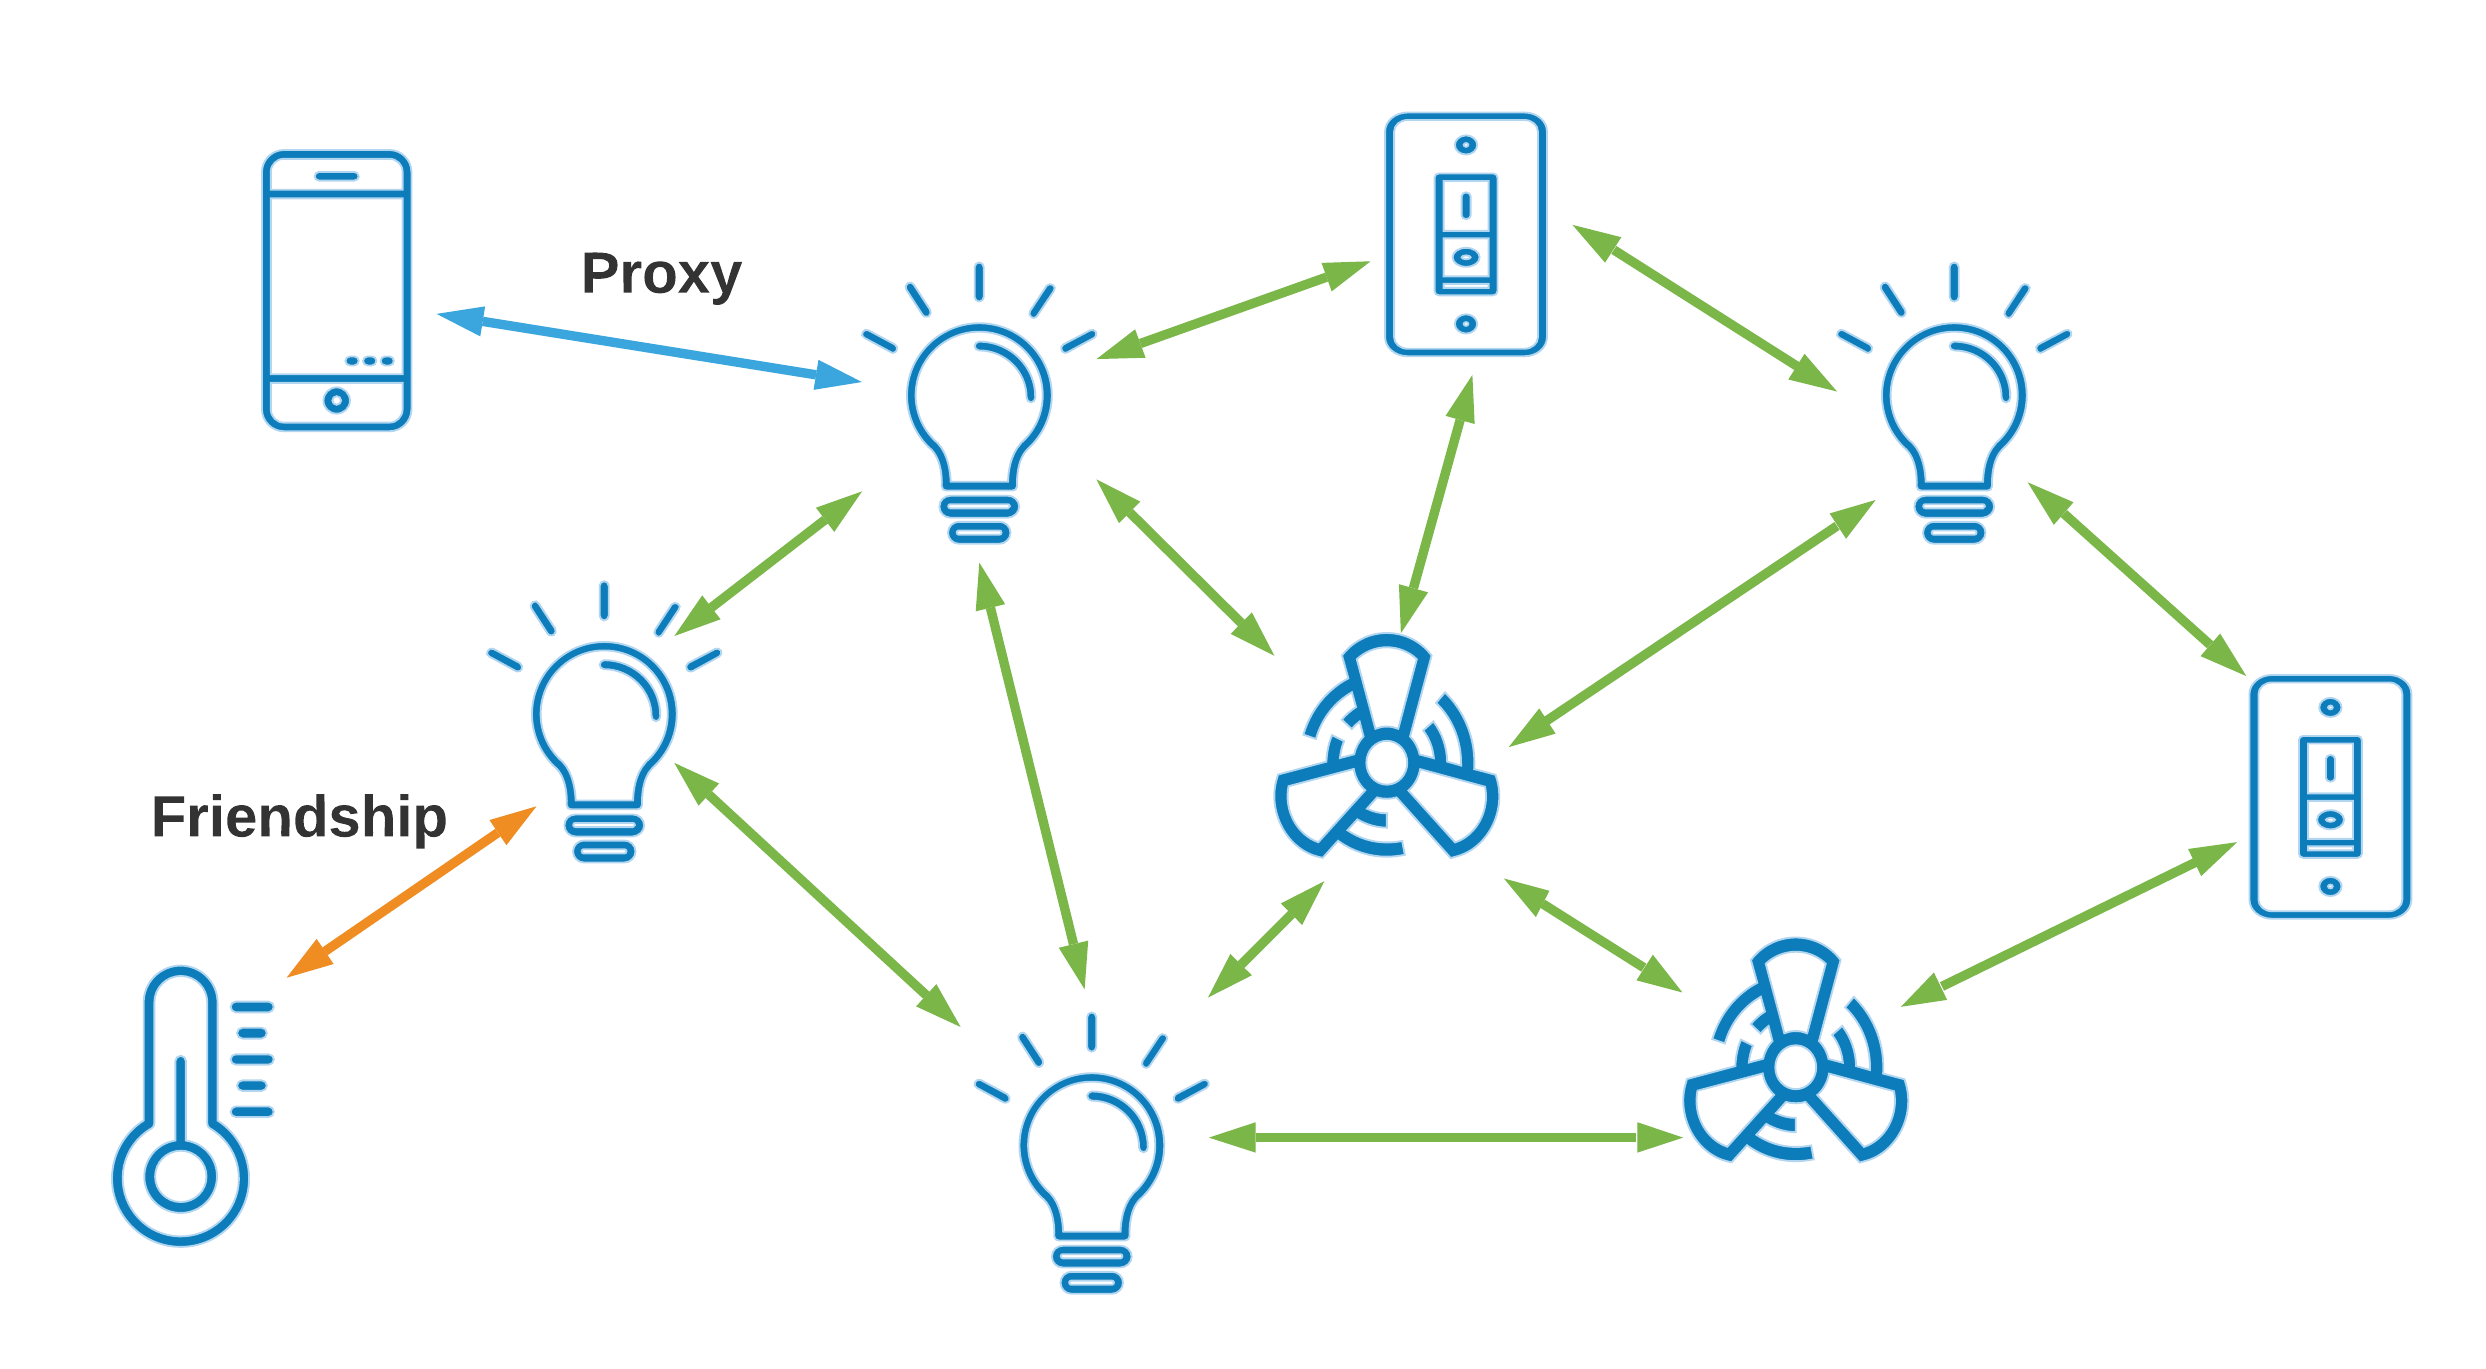
\includegraphics[width=0.8\textwidth]{./images/mesh_profile_features.png}
		\caption{Exemple \textit{Mesh Profile} \cite{Mesh Profile}}
	\end{center}
\end{figure}

Per facilitar la introducció del \textit{Mesh Profile} en desplegaments de BLE ja existents es defineix un mode d'operació anomenat intermediari (\textit{proxy}, en anglès).
El mode intermediari permet a un node d'una xarxa establir una connexió utilitzant BLE amb un altre node que no implementa el \textit{Mesh Profile}.
Així, un node antic pot ser perfectament controlat a través d'una \textit{Scatternet}.

Tenir una xarxa de nodes que reenvien paquets quan alguns dels nodes són de baix consum i amb poca capacitat de processament pot suposar problemes.
És per això que, el \textit{Mesh profile} inclou la possibilitat de definir una connexió d'amistat on el node de baix consum és l'amic.
Aquest dispositiu amic no haurà d'estar escoltant constantment sinó que podrà requerir els paquets dirigits a ell quan es desperti.
L'altre node associat que tindrà més capacitat de processament, memòria i probablement estarà connectat a la xarxa elèctrica haurà d'emmagatzemar els paquets i reenviar-los quan siguin requerits.

\subsection{Pila}
El \textit{Mesh Profile} defineix les capes de la seva pròpia pila.
En la capa inferior d'aquesta pila hi conté tot BLE, ja que el \textit{Mesh Profile} utilitza BLE per enviar paquets entre els nodes que formen la xarxa.
A continuació, es comentarà breument les diferents capes.

\begin{figure}[!h]
	\begin{center}
		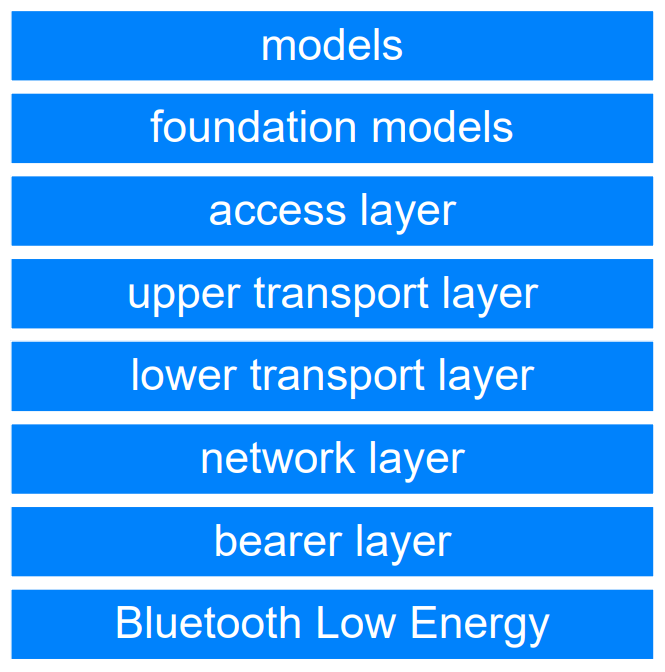
\includegraphics[width=0.6\textwidth]{./images/mesh_profile_stack2.PNG}
		\caption{Arquitectura del \textit{Mesh Profile} \cite{Mesh Profile Overview}}
		\label{mesh_netowrk_stack}
	\end{center}
\end{figure}

La capa \textit{Bearer} controla la transmissió i recepció de paquets, hi ha dos tipus, l'\textit{Advertising Bearer} i el GATT \textit{Bearer}.
L'\textit{Advertising Bearer} utiliza el BLE per enviar i rebre missatges corresponents al \textit{Mesh Profile}.
En canvi, el GATT \textit{Bearer} és el que s'utilitza per interactuar amb dispositius que no implementen el \textit{Mesh Profile} utilitzant el protocol d'intermediari comentat anteriorment.

La capa de xarxa defineix l'ús d'adreces i la gestió de les múltiples interfícies que pot tenir un node.
Les funcions de repetidor s'implementen en aquesta capa.
La capa de transport inferior realitza la segmentació i reassemblatge dels paquets que no caben en una PDU de transport.
La capa de transport superior és responsable de la seguretat, proveeix encriptació i autenticació.
Igualment, també s'encarrega de la funcionalitat d'amistat entre dispositius comentada anteriorment.
En la capa d'accés es defineix el format de les dades de la capa de transport incloent quina encriptació s'ha de realitzar entre d'altres.
Les dues capes superiors tracten la implementació dels models, els missatges i estats que defineix l'estàndard.

Comparant les capes de \textit{Mesh Profile} i de BLE (Figura \ref{mesh_netowrk_stack} i Figura \ref{host_stack} respectivament) es pot observar que són similars fins al punt que s'estan realitzant les mateixes funcions.
Això es deu al fet que en lloc de substituir o estendre BLE amb el \textit{Mesh Profile}, el que s'ha fet és mantenir BLE tal com està i afegir \textit{Mesh Profile} per sobre.
D'aquesta manera s'assegura la compatibilitat entre dispositius que implementen el \textit{Mesh Profile} i dispositius que no.
A més a més, és compatible tant amb BLE 5 com amb BLE 4, així que és molt fàcil afegir dispositius amb \textit{Mesh Profile} en una instal·lació ja existent.

\subsection{Seguretat}
En la majoria de tecnologies que s'han vist fins ara, incloent-hi BLE la seguretat és opcional per permetre implementacions simples del protocol que no la requereixen.
Aquest no és el cas del \textit{Mesh Profile} que obliga a utilitzar seguretat segons l'estàndard.

Tots els paquets corresponents al \textit{Mesh Profile} estan encriptats i autenticats.
Per fer-ho existeixen les claus de xarxa que són compartides entre tots els nodes de la mateixa xarxa i es requereixen per realitzar funcions de xarxa com reenviar paquets.
Amb aquestes claus s'ofusquen les capçaleres del paquet per donar privacitat de l'origen i destí envers un potencial actor maliciós que no pertany a la xarxa.
Si un node forma part d'una subxarxa, aquest també tindrà una altra clau única i compartida entre els nodes de la subxarxa.
Per tant, es poden aïllar certes parts de la xarxa, per exemple, una estança d'un d'hotel.

Cada xarxa pot tenir múltiples aplicacions que tindran la seva pròpia clau d'aplicació.
Aquesta servirà per aïllar diferents elements d'una xarxa que estan relacionats com poden ser els elements d'il·luminació (llums i interruptors) dels elements de calefacció (sensor de temperatura i radiador).

Finalment, tots els nodes contenen una clau de dispositiu que els permet formar part d'una xarxa o una aplicació.
Quant un dispositiu es vol eliminar de la xarxa o aplicació, per exemple, per vendre'l, es procedeix de forma segura afegint aquella clau a una llista negra.
Els dispositius que estan a la llista negra no se'ls renoven les claus d'aplicació o xarxa i per tant no poden seguir participant en les comunicacions.
Tal com és habitual s'utilitzen identificadors seqüencials en els paquets per evitar atacs de repetició on l'atacant retransmet un paquet per intentar repetir una acció anterior.


\chapter{Desenvolupament}
\section{Placa base CC1352R1}
Per analitzar el protocol BLE i veure les seves característiques s'ha utilitzat el kit per desenvolupament ràpid del microcontrolador CC1352R1.
\begin{figure}[h!]
	\begin{center}
		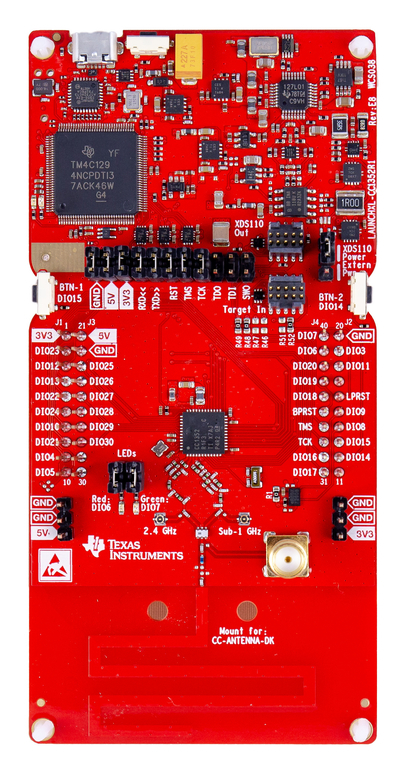
\includegraphics[width=0.5\textwidth]{./images/launchxl-cc1352r1.jpg}
		\caption{Placa \cite{placa}}
	\end{center}
\end{figure}

Aquesta placa permet el desenvolupament d'aplicacions en BLE utilitzant el microcontrolador CC1352 de Texas Instruments a continuació es descriuen les seves característiques principals \cite{placa_datasheet}.

El dispositiu CC1352R és multiprotocol i multibanda orientat a 2.4 GHz o sub-1GHz que serveix per a Thread, Zigbee, Bluetooth 5 Low Energy, IEEE 802.15.4g i 6LoWPAN. Pel que fa a memòria té 352 KB flash programable, 256 KB de ROM per a protocols i llibreries, 8 KB de Cache SRAM i 80 KB de RAM protegida amb paritat.
Pel que fa als perifèrics el més important és el ADC de 12 bits i 8 canals amb freqüència de mostreig de 200 Kmostres/s (multiplexat). També té Rellotge de Temps Real (RTC), acceleradors de operacions criptogràfiques i generador de números aleatoris.
La radio multibanda que té te un receptor amb sensibilitat de -121 dBm per a sub-1GHz i de -110 dBm a 50 Kbps o -105 dBm a 125 Kbps. El transmissor pot transmetre fins a 14 dBm sub-1GHz i 5dBm a 2.4 GHz.


\section{Software}
Per al desenvolupament de projectes per a la placa s'ha utilitzat el entorn de desenvolupament Code Composer Studio. El software és el SimpleLink(TM) CC13X2.
[Comentar tema versió]

\section{Project 0}
El Project 0 és el projecte instal·lat amb que les plaques vénen de fàbrica. Aquest projecte exposa certs serveis a través de BLE i et permet veure una comunicació simple entre la placa i un dispositiu mòbil.
La comunicació es fa a través del control dels dos LEDs que te la placa (els LEDs que estan directament controlats pel microcontrolador) i també per l'estat dels botons que hi ha a ambdós costats de la placa.
*Aquest projecte també inclou altres serveis en que no entrarem.

Aquest projecte serveix per tenir un bon exemple de com està dissenyada l'arquitectura dels serveis amb les seves característiques amb una relativa simple funcionalitat. A continuació s'analitzaran diferents parts dels atributs.

\subsection{Serveis de Butons i LEDs}

En la següent taula es poden veure tots els valors que hi ha tal i com estan en la taula d'atributs del servidor GATT.
Per facilitar la visualització de les dades s'han tret els zeros finals dels UUIDs propis però cal recordar que en total tenen 16 parells (128 bits en representació hexadecimal) i no només els 9 parells que surten a la taula.

\begin{center}
	\begin{table}[h!]
		\csvautotabular{data_files/projectzeroUUID.csv}
	\end{table}
\end{center}

Per poder entendre els atributs, al tenir UUID propis és necessari tenir en compte la documentació amb la que s'ha desenvolupat aquest projecte.

\begin{figure}[h!]
	\begin{center}
		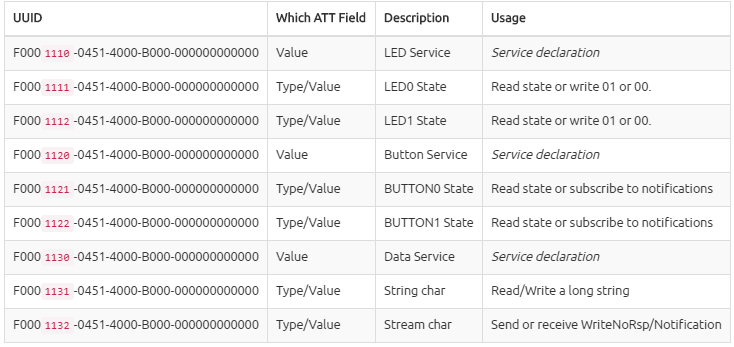
\includegraphics[width=\textwidth]{./images/Project_0_UUID.png}
		\caption{Definició dels UUIDs}
	\end{center}
\end{figure}

El primer que cal tenir clar és que en taula anterior (afegir link dinàmic) els valors estan representats amb l'ordre en que es reben i en general els serveis estandarditzats (i també aquest servei propi) utilitza \textit{little-endian} per enviar la informació.
Això resulta en que els caràcters hexadecimals queden (per parelles) ordenats al revés.

Al analitzar els atributs es pot veure com aquells que tenen el UUID 0x2800 en el seu valor només tenen un UUID corresponent al les definicions de serveis de LEDs i de botons.
Seguidament, als atribut amb UUID 0x2803 hi ha les definicions de les característiques, en el seu valor hi ha múltiples parts.
El primer parell hexadecimal correspon a les propietats. Just després hi ha dos parells hexadecimals que identifiquen el \textit{Handle} del atribut on hi ha la característica.
I per últim la resta de caràcters corresponen al UUID que identifica la característica.

\subsection{Propietats}
Les propietats d'accés són un valor que identifica quines operacions i procediments es poden fer sobre la característica.
El camp té 8 bits per defecte i cada un d'ells identifica una operació o procediment.
Es poden combinar qualsevol quantitat d'aquests bits per habilitar múltiples opcions.

\begin{center}
	\begin{tabular}{|c|c|l|}
		\hline
		Binary	&	Hex		&	Property	\\	\hline
		0000 0001	&	0x01	&	Broadcast\\	\hline
		0000 0010	&	0x02	&	Read	\\	\hline
		0000 0100	&	0x04	&	Write w/o Response	\\	\hline
		0000 1000	&	0x08	&	Write	\\	\hline
		0001 0000	&	0x10	&	Notification w/o ACK	\\	\hline
		0010 0000	&	0x20	&	Indication with ACK	\\	\hline
		0100 0000	&	0x40	&	Signed Writes	\\	\hline
		1000 0000	&	0x80	&	Aditional Properties	\\	\hline
	\end{tabular}
\end{center}

Primer de tot cal destacar la implementació de comunicacions amb o sense reconeixement. D'aquesta manera si preferim reduir la quantitat de missatges per estalviar bateria enlloc d'assegurar-se que s'ha rebut la informació es dona la opció.

Pel que fa les propietats en el Project 0 les característiques dels LEDs tenen el valor 0x0E que resulta en 0000 1110 per tant, es permet: llegir, escriure i escriure sense resposta.
En canvi les característiques del servei de botons té el valor 0x12 que suposa 0001 0010, per tant, es permet notificació sense reconeixement.

La notificació i indicació són funcions que ajuden a reduir el consum de recursos.
Quan volem saber en quin estat estan els botons de la placa contínuament es podria anar llegint el estat de la característica constantment però això suposarien molts missatges i reduiria el temps que els dispositius es poden adormir i així ser més eficients.
Per evitar aquest cas es pot configurar la característica tal que sigui la mateixa placa qui enviï el missatge automàticament quant el estat de la característica canviï.
D'aquesta manera el receptor només cal que escolti els missatges de la placa per tal de saber en quin estat està el botó.

En cas de que es vulgui indicació amb reconeixements és possible configurar-ho d'aquesta manera a través del atribut Configuració de Característica del Client identificat amb el UUID 0x2902 i estandarditzat en la especificació de Bluetooth.
Si el valor és 0 no hi ha transmissions, si el valor és 1 s'envien notificacions (sense reconeixement) i si el valor és 2 s'envien indicacions (notificacions amb reconeixement). 

El bit d'extensió de propietats, en cas que sigui 1 indica que existeix un atribut: Descriptor Propietats Esteses de Característica.
Aquest atribut te el UUID 0x2900 i el que permet és afegir més propietats de les que poden existir amb el espai limitat de 8 bits que hi ha per defecte.
Aquest sistema permet afegir fins a 16 bits més per indicar propietats, actualment estan els dos primers definits segons el estàndard i la resta estan reservats per a ús futur \cite{extended properties}.

Aquests 2 primers que estan definits són escriptura fiable i escriptura auxiliar.
L'escriptura fiable permet escriure valors amb un procediment diferent al habitual que permet assegurar-se que el valor que es vol modificar s'ha escrit i no hi han hagut errors.
Pel que fa  al'escriptura auxiliar permet escriptura al descriptor de característica [posar exemple].

\section{Experimentació}
Per comprendre millor com afecten els diferents paràmetres configurables corresponents a BLE i també les prestacions dels perifèrics de la placa es realitzaran els següents escenaris.

\subsection{ADC}
La placa té un convertidor analògic-digital que ens permetrà enviar senyals analògiques un cop s'han digitalitzat.


\subsection{Range}
\subsection{Throughput}
\chapter{Experimental}
\section{ADC}
\section{Range}
\section{Throughput}
\chapter{Projecte de sensors}
En aquest capítol es realitzarà un escenari real on s'implementarà la tecnologia BLE per transmetre dades.
Primerament es realitzaran proves per mesurar les capacitats del protocol i de la PCB utilitzats.

\section{Experimentació}
A fi d'entendre millor com afecten els diferents paràmetres configurables corresponents a BLE i també les prestacions dels perifèrics de la PCB, s'han realitzat els següents escenaris.


\subsection{Abast}

Com ja s'ha mencionat anteriorment l'abast teòric que té BLE, 100-200 metres, és considerable comparat amb tecnologies similars.
Però, cal entendre que, a l'estar utilitzant la banda de 2.4 GHz, l'abast de BLE dependrà de l'entorn, on pot haver-hi molta variabilitat d'interferències.
A causa d'això, en un escenari realista l'abast que es pot assolir pot ser molt diferent del teòric.
Les LAUNCHXL-CC1352R1 utilitzades en aquest projecte, per si soles, no són l'eina perfecta per fer proves d'abast.
Això es deu, en part, a què no és possible transmetre a la màxima potència permesa per l'estàndard que és de fins a 20 dBm.
El límit és de 5 dBm i per defecte només s'utilitzen 0 dBm de potència en transmissió.

Per realitzar un experiment que fos més precís seria avantatjós utilitzar una antena externa més directiva.
En lloc d'analitzar l'abast de la tecnologia en aquest apartat es farà un balanç comparatiu per comprovar les diferències reals d'utilitzar les diferents capes físiques de BLE.

Per a aquest apartat s'ha realitzat un experiment pràctic en un lloc relativament aïllat i on es pogués tenir una suficient distància amb visibilitat directa.
S'ha escollit un pàrquing i utilitzat la potència per defecte de 0 dBm per poder treballar amb distàncies més curtes.

\begin{figure}[!h]
	\begin{center}
		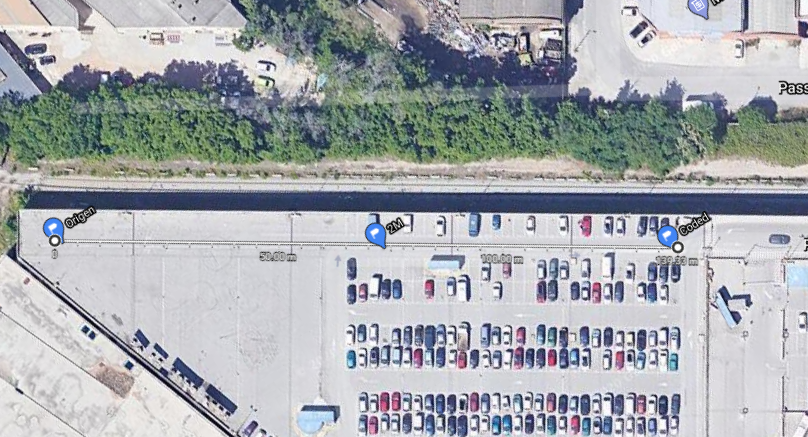
\includegraphics[width=\textwidth]{./images/prova_abast.png}
		\caption{Abast real de BLE}
		\label{abast}
	\end{center}
\end{figure}

El procediment per realitzar l'experiment va ser col·locar una de les plaques sobre un cotxe i amb l'altre connectada a un altre ordinador anar retrocedint fins que es perdés la connexió.
Per forçar que es perdés la connexió quan ja no es podia establir una comunicació des de la PCB que s'anava movent s'anaven enviant peticions de lectura d'atributs.

Els resultats obtinguts, que es poden veure en la Figura \ref{abast}, indiquen que la distància màxima d'abast del dispositiu en una capa 2M és de 75 metres, mentre que en una capa S=8 aquesta distància s'estén fins als 135.
S'han tingut en compte únicament aquestes capes físiques, ja que com que no hi ha interferències significatives i sempre s'ha mantingut la visibilitat directa, els resultats de la capa 1M són similars als de 2M i els de Coded S=2 són similar als de S=8.

També s'ha realitzat un mapa de cobertura d'un interior d'una casa per poder observar quin és l'abast quan es tenen en compte les parets.
En aquest cas s'ha establert una connexió fins a la PCB i s'ha obtingut el valor de la potència rebuda en totes les estàncies de la casa. De les mesures preses s'ha realitzat un mapa de cobertura que es pot veure a la Figura \ref{heatmap}.

La PCB s'ha col·locat a l'habitació 1 i s'ha configurat amb la potencia de transmisió de 0 dBm i amb la capa física LE 1M.
Just al costat de la PCB es reben -50 dBm i en l'altre punta de l'habitació hi ha -70 dBm, això es deu, als obstacles que hi ha entre mig.
Al llarg del passadís la potència és de -62 dBm, és bona ja que es la zona on hi ha visibilitat directe entre els dispositius.
A les estàncies adjuntes al passadís, el lavabo i l'habitació 2 la potència arriba a baixar fins a -80 dBm.

Més enllà a la cuina i al menjador es reben potències de -80 fins a -85 dBm.
A partir del rebedor la senyal ja es veu greument afectada i es comencen a perdre alguns paquets. En aquesta estància es reben -90 dBm. A l'habitació 3, la connexió és molt pobre i és habitual que els dispositius perdin la connexió. En aquesta, la potència rebuda es d'entre -95 dBm i -100 dBm.
En el vestidor i el lavabo 2, que són les estàncies més allunyades de la casa. En aquestes al creuar la porta sempre es perd la connexió.
Que es rebi connexió arribi a l'habitació 3 i no al lavabo i vestidor del costat es deu a que el senyal pentera la paret i arriba més fàcilment.

Tal i com es pot observar pel resultat, BLE pot aconseguir una abast considerable en interiors però no d'una punta a un altre de la casa.
En aquest escenari específic la configuració era adverda a propòsit per veure quin era el límit de la tecnologia.
En un cas més realista, hi hauria un receptor al centre de la casa que tindria una cobertura que abarcaria qualsevol punt.
D'aquesta manera qualsevol sensor situat a les puntes de la casa tindria connectivitat sense problemes.
\newpage

\begin{figure}[!h]
	\begin{center}
		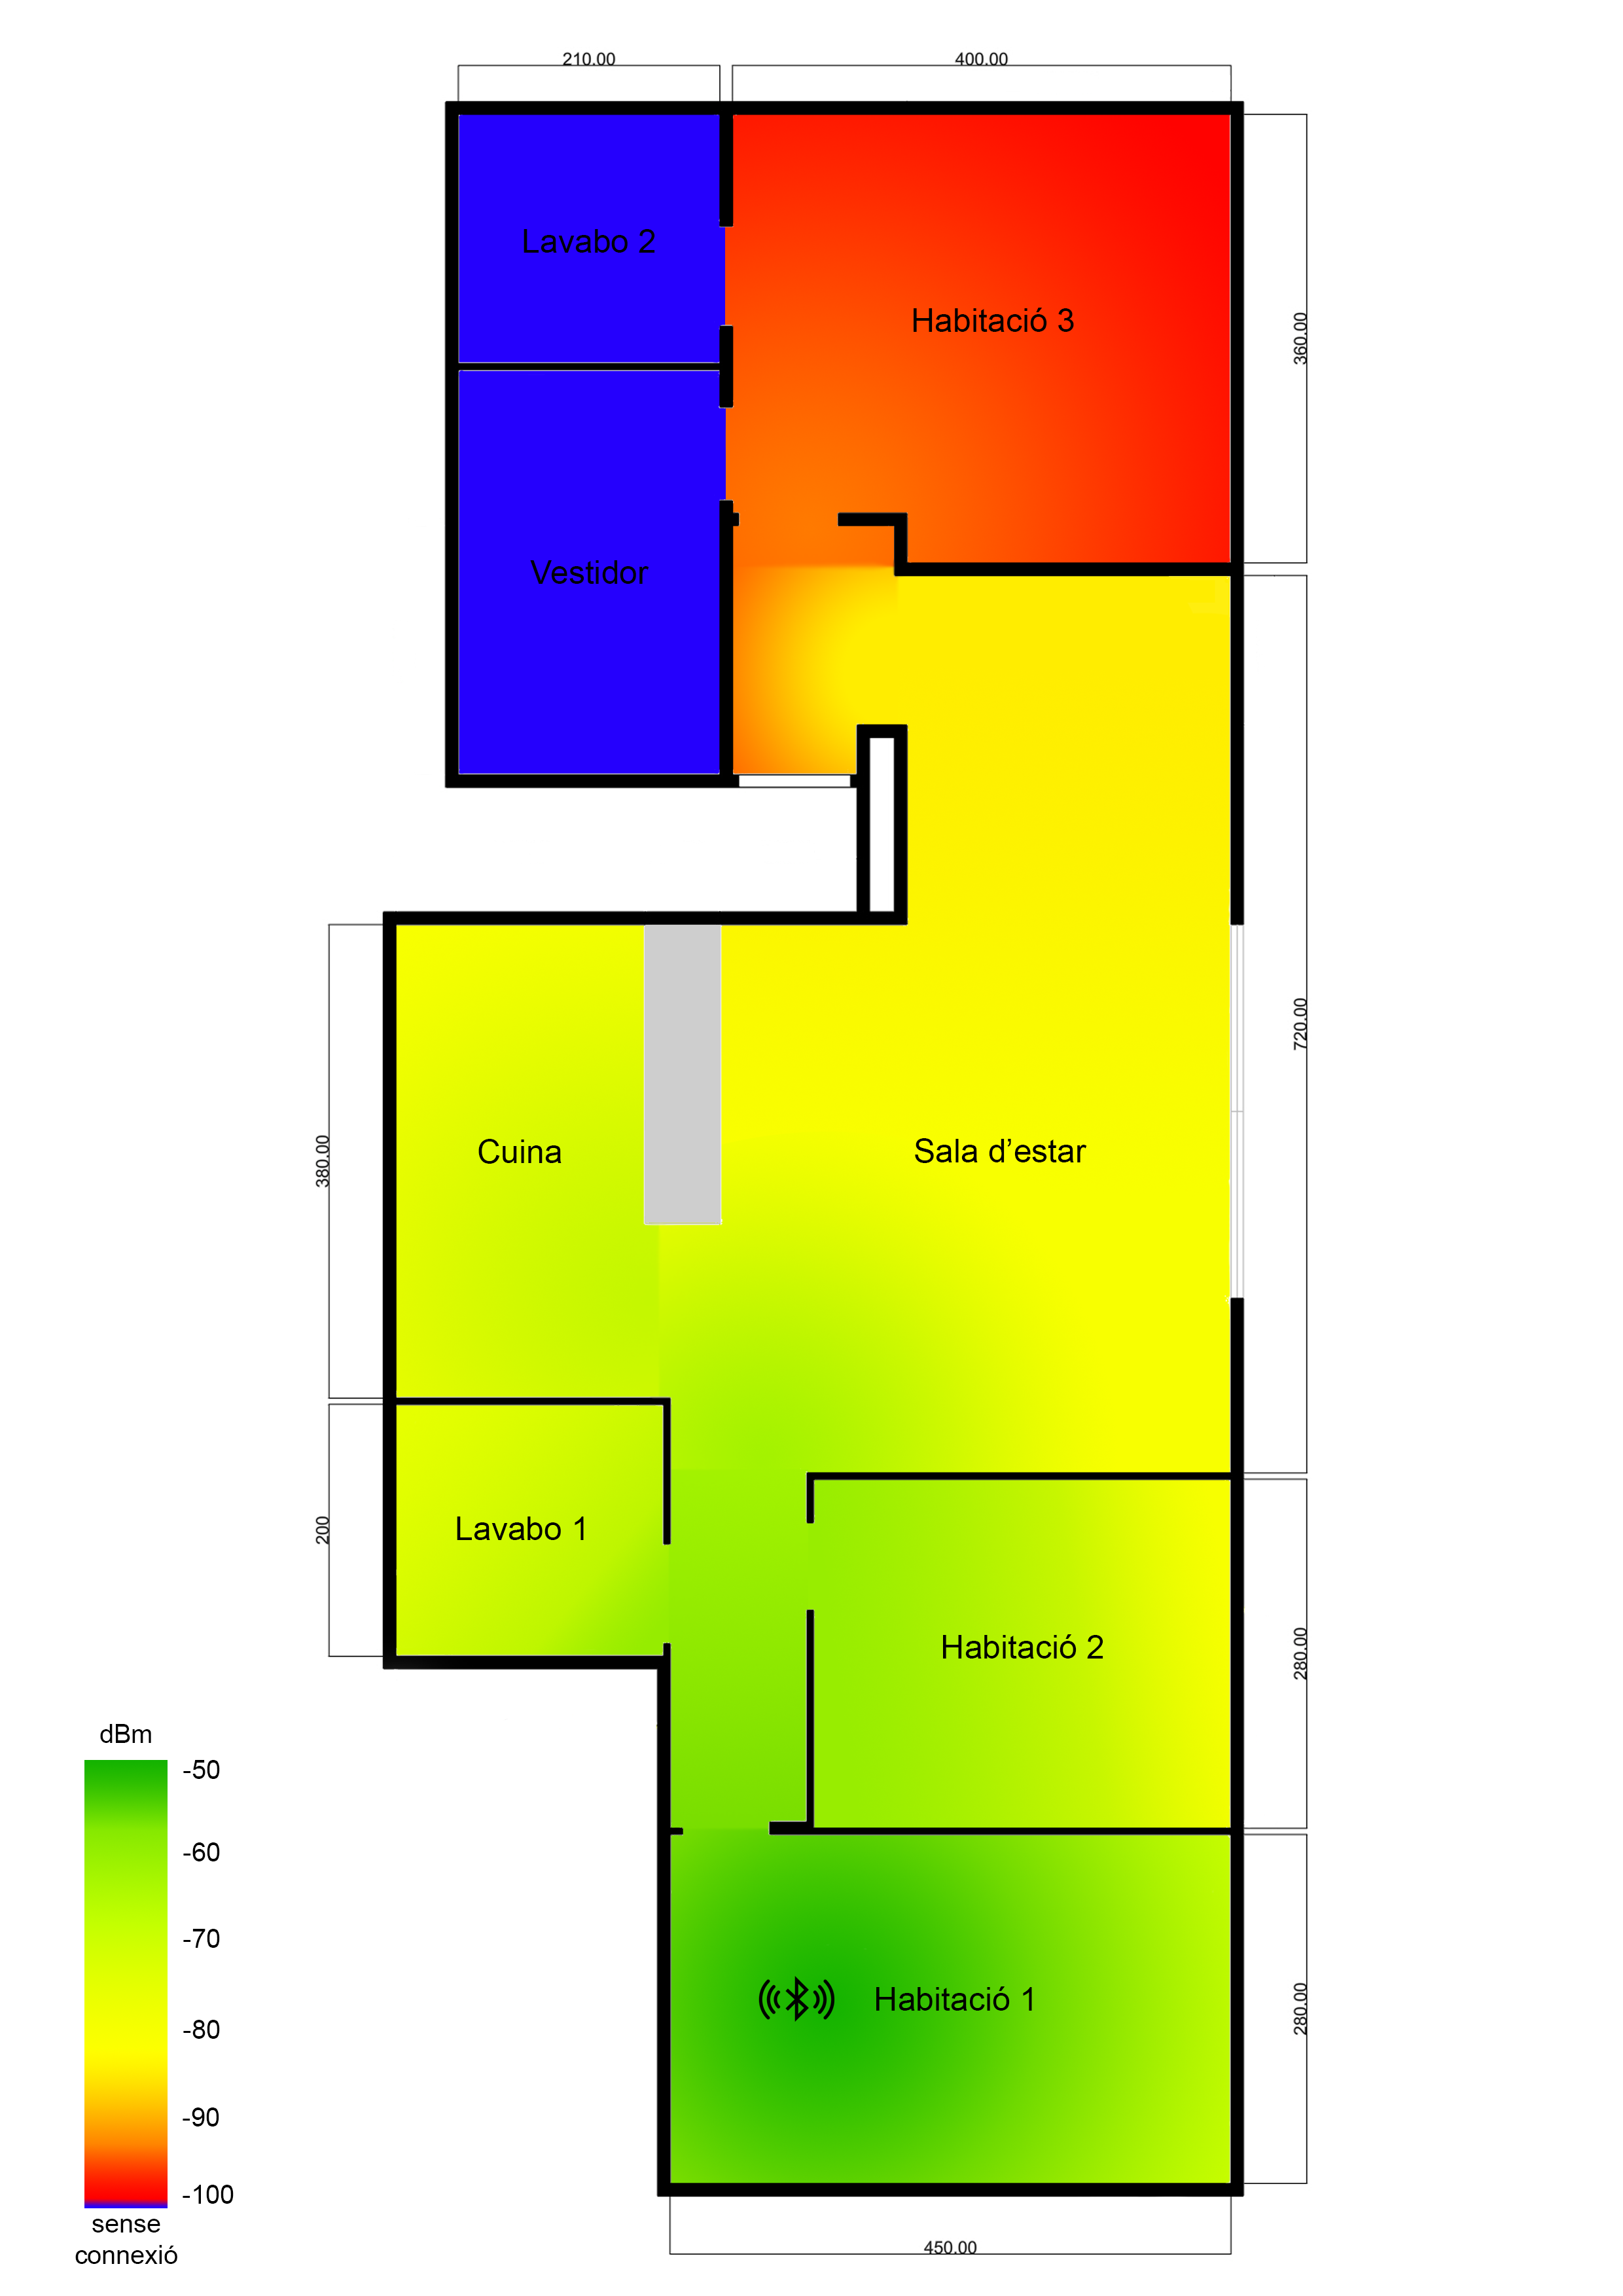
\includegraphics[width=\textwidth]{./images/hotmap.png}
		\caption{Mapa de cobertura}
		\label{heatmap}
	\end{center}
\end{figure}

Així doncs, en aquest apartat s'ha vist una de les millores de la capa física Coded, l'abast.
Però també cal recordar que on és extremadament útil és en el de resistència a les interferències.

\subsection{Consum d'energia}

El consum dels dispositius que utilitzen BLE és la característica més significativa, ja que, aquesta tecnologia està dissenyada per a consumir la menor quantitat d'energia possible.
Les plaques utilitzades tenen ponts extraïbles, tal com es pot veure en la Figura \ref{ponts_extraibles}, que permeten desconnectar els components que no són essencials per al funcionament del xip CC1352R.

\begin{figure}[h]
	\begin{center}
		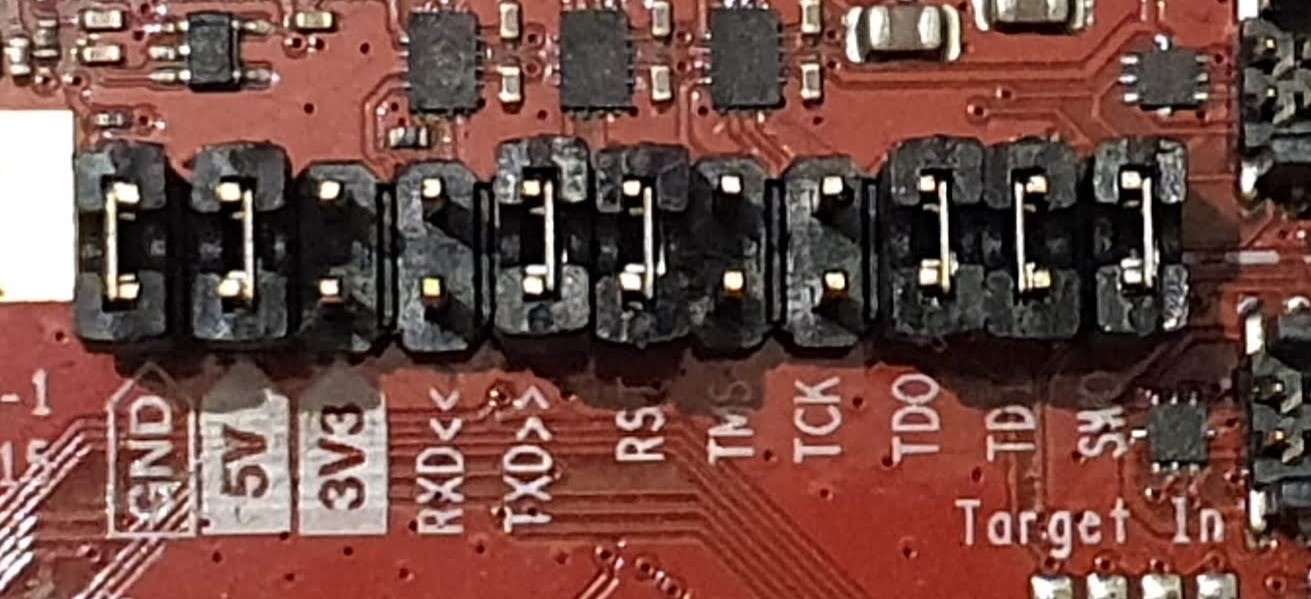
\includegraphics[width=0.7\textwidth]{./images/ponts.jpg}
		\caption{Ponts extraïbles de la PCB}
		\label{ponts_extraibles}
	\end{center}
\end{figure}

D'aquesta manera, es pot utilitzar un analitzador de potència per mesurar l'energia consumida.
Aquesta configuració produeix una mesura molt precisa i permet calcular el cicle de vida del dispositiu que s'està desenvolupant.
Per contra, no es poden utilitzar les eines de desenvolupament com la depuració del codi.
Aquesta configuració no ha estat possible realitzar-la a causa de la situació sanitària actual.

Per poder desenvolupar fàcilment un projecte i analitzar els canvis que el codi produeix en l'ús d'energia, existeix una eina anomenada Energy Trace.
D'aquesta manera, es pot analitzar comparativament en quin moment s'està consumint l'energia i es poden adaptar els paràmetres de la connexió per observar quin serà l'estalvi que s'aconseguirà.
És per això que, es poden prendre les decisions de quins sacrificis són assumibles, per exemple, augmentar la latència a canvi de reduir el consum.
Aquesta eina però, no substitueix la solució explicada anteriorment amb l'analitzador de potència, ja que l'Energy Trace resulta molt menys precisa.

Per provar el funcionament de l'Energy Trace s'ha utilitzat durant l'execució en el xip del Project Zero.
A la Figura \ref{energy_trace1} es pot observar una captura del consum aproximat de corrent.

\begin{figure}[!h]
	\begin{center}
		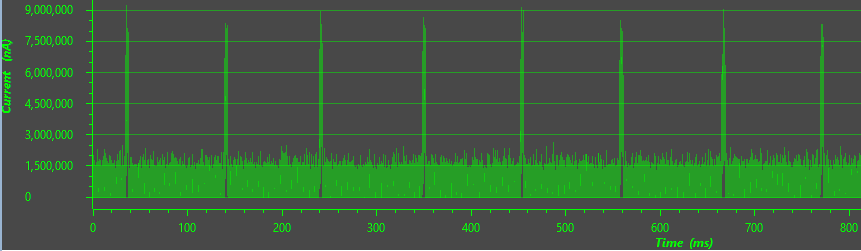
\includegraphics[width=\textwidth]{./images/consum_energia_no_connected_current2.png}
		\caption{Mesura de corrent sense connexió}
		\label{energy_trace1}
	\end{center}
\end{figure}

És possible visualitzar com hi ha pics de consum cada 100 ms, aquests corresponen als instants en què el dispositiu està enviant els anuncis.
Aquests 100 ms corresponen a l'interval d'anunci que s'ha configurat per a aquest projecte.

També és possible mesurar el consum d'energia acumulada de la PCB al llarg del temps, en aquest cas s'ha realitzat durant un segon i es pot veure a la Figura \ref{energy_measure}.

\begin{figure}[!h]
	\begin{center}
		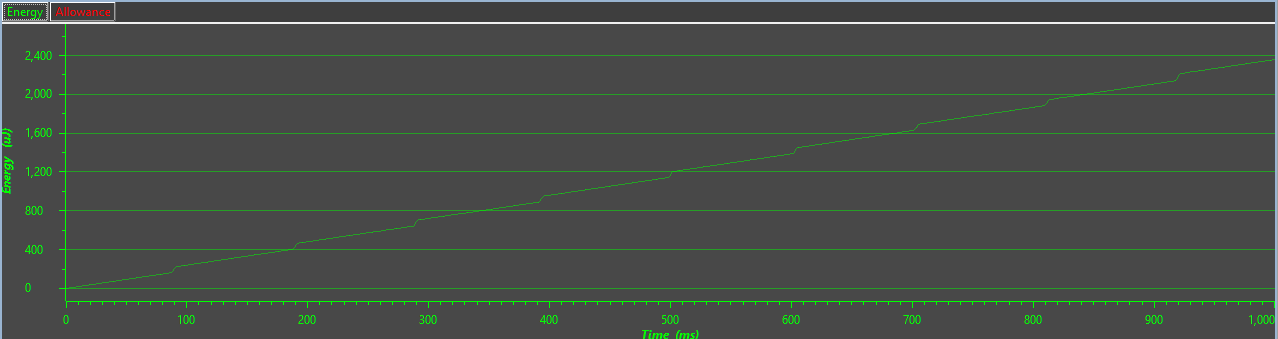
\includegraphics[width=\textwidth]{./images/consum_energia_no_connected_energia.PNG}
		\caption{Mesura d'energia sense connexió}
		\label{energy_measure}
	\end{center}
\end{figure}

Un cop s'estableix una connexió amb el dispositiu es realitza una altra captura del corrent que es pot observar a la Figura \ref{energy_trace_connection}.

\begin{figure}[!h]
	\begin{center}
		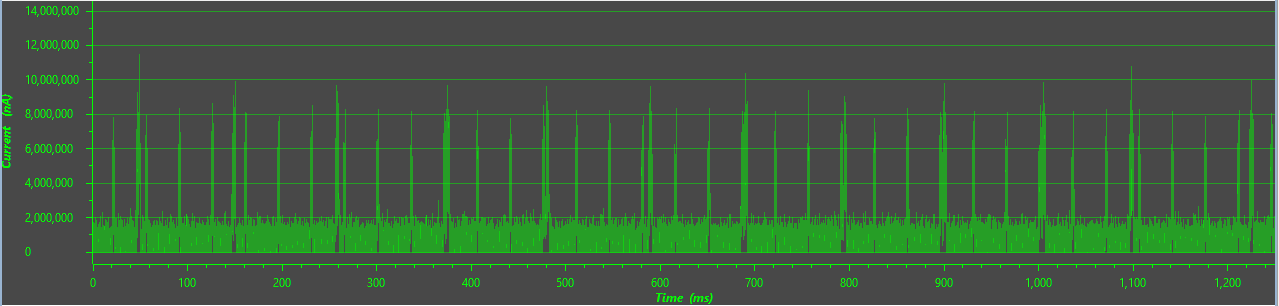
\includegraphics[width=\textwidth]{./images/consum_energia_connected_current.png}
		\caption{Mesura de corrent amb connexió}
		\label{energy_trace_connection}
	\end{center}
\end{figure}

A la gràfica és possible veure com segueixen estant els pics cada 100 ms però també n'hi ha cada 40 ms.
Aquests, darrers, es deuen als esdeveniments de connexió que en aquest cas estan configurats perquè es produeixen cada 40 ms.

En aquestes captures de consum de corrent, tot i que hi ha molta variació, es pot comprovar que mentre no es transmeten paquets, el consum és d'entre 0 i 2 mA.

També, es realitza una captura del consum d'energia acumulat durant un segon:

\begin{figure}[!h]
	\begin{center}
		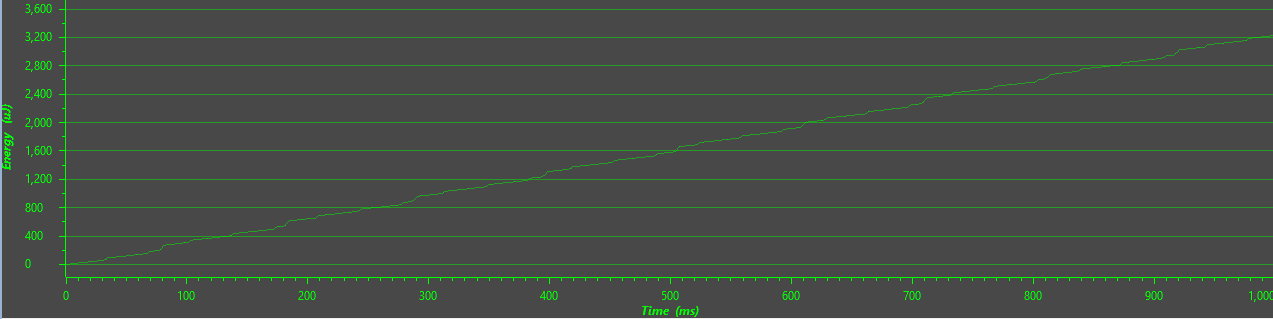
\includegraphics[width=\textwidth]{./images/consum_energia_connected_energy.png}
		\caption{Mesura d'energia amb connexió}
		\label{energy_trace2}
	\end{center}
\end{figure}

Els màxims que es produeixen per anuncis i per esdeveniments de connexió poden semblar similars en les captures de consum de corrent.
Tanmateix, no és així, en les captures de consum d'energia es pot observar com hi ha increments més pronunciats corresponents als anuncis i en canvi els esdeveniments de connexió els increments són més lleugers.

Si es veuen amb més detall l'anunci i l'esdeveniment es pot observar com són d'una duració diferent.
D'una banda, l'anunci dura uns 4 mil·lisegons i mig, en canvi l'esdeveniment de connexió només dura 2 mil·lisegons.
\newline
\begin{figure}[!h]
	\begin{center}
		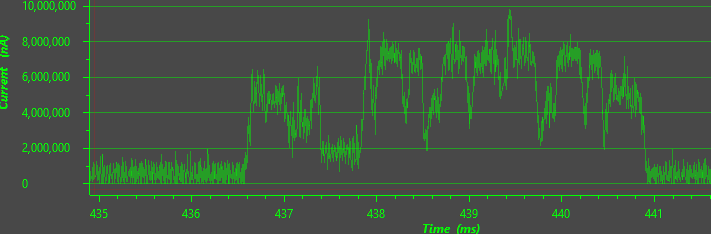
\includegraphics[width=\textwidth]{./images/pic_anunci_captura.png}
		\caption{Captura d'anunci}
		\label{energy_trace_adv}
	\end{center}
\end{figure}
\begin{figure}[!h]
	\begin{center}
		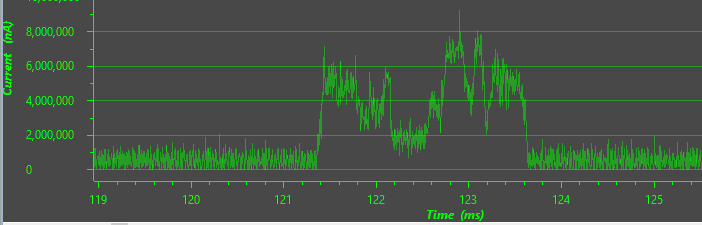
\includegraphics[width=\textwidth]{./images/pic_connectat_captura.png}
		\caption{Captura d'esdeveniment}
		\label{energy_trace_event}
	\end{center}
\end{figure}

Aquesta eina, per tant, està orientada a facilitar una idea comparativa d'en quins instants es consumeix més energia.
D'aquesta manera, és més fàcil pel desenvolupador comprovar com els canvis en el codi afecten el consum d'energia.

A part dels gràfics, l'Energy Trace també proporciona directament les dades més rellevants de les captures.
A la taula \ref{taula_consum} es troben els valors importants.\newline

\begin{table}[h!]
	\begin{center}
	\resizebox{\textwidth}{!}{%
		\renewcommand{\arraystretch}{2}
		\begin{tabular}{l|c|c|c|c|c|c|c|}
			\cline{2-8}
			\multirow{2}{*}{}                    & \multirow{2}{*}{\begin{tabular}[c]{@{}c@{}}Temps de Mesura\\ (s)\end{tabular}} & \multirow{2}{*}{\begin{tabular}[c]{@{}c@{}}Energia\\ (mJ)\end{tabular}} & \multicolumn{2}{c|}{Potència (mW)} & \multicolumn{2}{c|}{Corrent (mA)} & \multirow{2}{*}{Temps de Vida} \\ \cline{4-7}
			&                                                                                &                                                                         & mitjana          & màxim           & mitjana          & màxim          &                                \\ \hline
			\multicolumn{1}{|r|}{Sense Connexió} & 10                                                                             & 23,87                                                                   & 2,387            & 34,566          & 0,723            & 10,475         & 11 dies i 12 hores             \\ \hline
			\multicolumn{1}{|r|}{Amb Connexió}   & 10                                                                             & 32,57                                                                   & 3,257            & 41,672          & 0,987            & 12,63          & 8 dies i 10 hores              \\ \hline
		\end{tabular}%
		\renewcommand{\arraystretch}{1}
	}
	\end{center}
	\caption{Taula comparativa de mesures\label{taula_consum}}	
\end{table}

Per aquests valors s'han pres mesures de 10 segons de duració per obtenir unes mitjanes més representatives d'un ús continu.
Es pot observar com la potència i corrent màxim consumits, tant amb connexió com sense, no són molt diferents entre si.
Això es deu al fet que independentment de si el dispositiu té conexions establertes, s'enviaran els anuncis que suposen el pic més important de les gràfiques amb el consum de corrent.

Els paràmetres amb els quals s'ha pres la mesura no estan optimitzats específicament per a un consum molt baix, tot i això, es pot observar com la mitjana de consum és molt reduïda, per sota d'1 mA.
Per contextualitzar com és de baix aquest consum, és habitual calcular un temps de vida estimat d'una pila de botó, en aquest cas s'utilitza la CR2032.
En aquest cas, el temps de vida, tenint en compte la connexió seria de 8 dies.
Altrament, sense connexió aquest temps de vida s'allargaria fins als onze dies i mig.
Per tant, el temps de vida s'assimilarà més a 8 o 11 dies depenent del temps en què el dispositiu es passi amb alguna connexió.

Per contextualitzar-ho més, si utilitzéssim una bateria habitual en els telèfons mòbils que tingués 3800 mAh suposaria un temps de vida de 160 amb connexió i 219 dies sense, uns 7,3 i 5,3 mesos corresponentment.

\section{Lectura de l'ADC}
El \textit{Analogic to Digital Converter} és un perifèric de la PCB que permet convertir un senyal analògic a un digital.
Per poder realitzar la lectura amb l'ADC, és necessari dissenyar un circuit per simular el senyal que produiria un sensor i també desenvolupar el codi necessari perquè la PCB prengui la mesura.
A continuació s'explicaran aquests processos.

\subsection{Disseny del simulador de sensors}
La PCB té un convertidor analògic-digital que ens permetrà enviar senyals analògics un cop s'han mostrejat.
En aquest treball no es tractaran directament els sensors sinó que es simularan els senyals que produirien.
Com que la PCB i el seu ADC treballen a 3,3$V$ es crearà un circuit que permeti controlar un voltatge d'entre 0 i 3,3$V$.

Aquest circuit es basarà en un divisor de voltatge simple format per una resistència i un potenciòmetre.
El potenciòmetre permet canviar la resistència de l'element a través d'un cargol i junt amb el circuit que l'envolta permetrà canviar el voltatge a la sortida.

\begin{figure}[!h]
	\begin{center}
		\begin{circuitikz}
			\draw
			(0,2) node[anchor=east] {$V_{in}$}
			to [R=$R_1$, *-] (2,2)
			to [vR=$R_{pot}$, *-] (2,0) node[tlground](GND){};
			\draw
			(2,2) to [short, -*] (3,2)
			to (3,2) node[anchor=west] (3,2) {$V_{out}$};
		\end{circuitikz}
		
	\end{center}
\end{figure}

Aquest circuit segueix l'estructura d'un divisor de voltatge per tant es pot calcular el voltatge a la sortida segons la següent fórmula.

\begin{equation}
	V_{in}\cdot\frac{R_{pot}}{R_1+R_{pot}}=V_{out}
\end{equation}

Per escollir els components cal tenir en compte utilitzar resistències de valor alt per reduir el consum d'energia.
S'utilitzarà un potenciòmetre de 10$k\Omega$ per tant serà una resistència que es podrà modificar des de 0$\Omega$ fins 10$k\Omega$.
Per trobar l'$R_1$ que compleixi els requisits queda la següent fórmula.

\begin{equation}
	R_1=5V\cdot\frac{10k\Omega}{3.3V}-10k\Omega\approx5151\Omega
\end{equation}

Per a l'$R_1$ s'utilitzaran resistències de la sèrie E12, els valors que més s'acosten a $5$,$121\Omega$ són $5.6k\Omega$ i $4.6k\Omega$.
Per assegurar-se que no es superen els 3.3$V$ a l'entrada de l'ADC que podria malmetre el dispositiu s'escull la resistència superior, per tant el circuit final s'ha dissenyat de la següent manera.

\begin{figure}[!h]
	\begin{center}
		\begin{circuitikz}
			\draw
			(0,2) node[anchor=east] {$5\,V$}
			to [R=$5.6\;k\Omega$, *-] (2,2)
			to [vR=$ \lbrack 0-10 \rbrack \;k\Omega$, *-] (2,0) node[tlground](GND){};
			\draw
			(2,2) to [short, -*] (3,2)
			to (3,2) node[anchor=west] (3,2) {$[0-3.3]\;V$};
		\end{circuitikz}
		
	\end{center}
\end{figure}

Com que s'utilitzaran 4 canals de l'ADC per mesurar, es necessiten 4 circuits com el que s'ha dissenyat.
S'ha implementat el circuit en una placa de proves i soldat els components de tal manera que cal connectar el voltatge d'entrada (a 5$V$) en vermell, terra en negre i finalment quatre cables blaus on hi haurà el voltatge controlat pels quatre potenciòmetres.
A la Figura \ref{protoboard} es pot observar aquesta implementació real del circuit.

\begin{figure}[!h]
	\begin{center}
		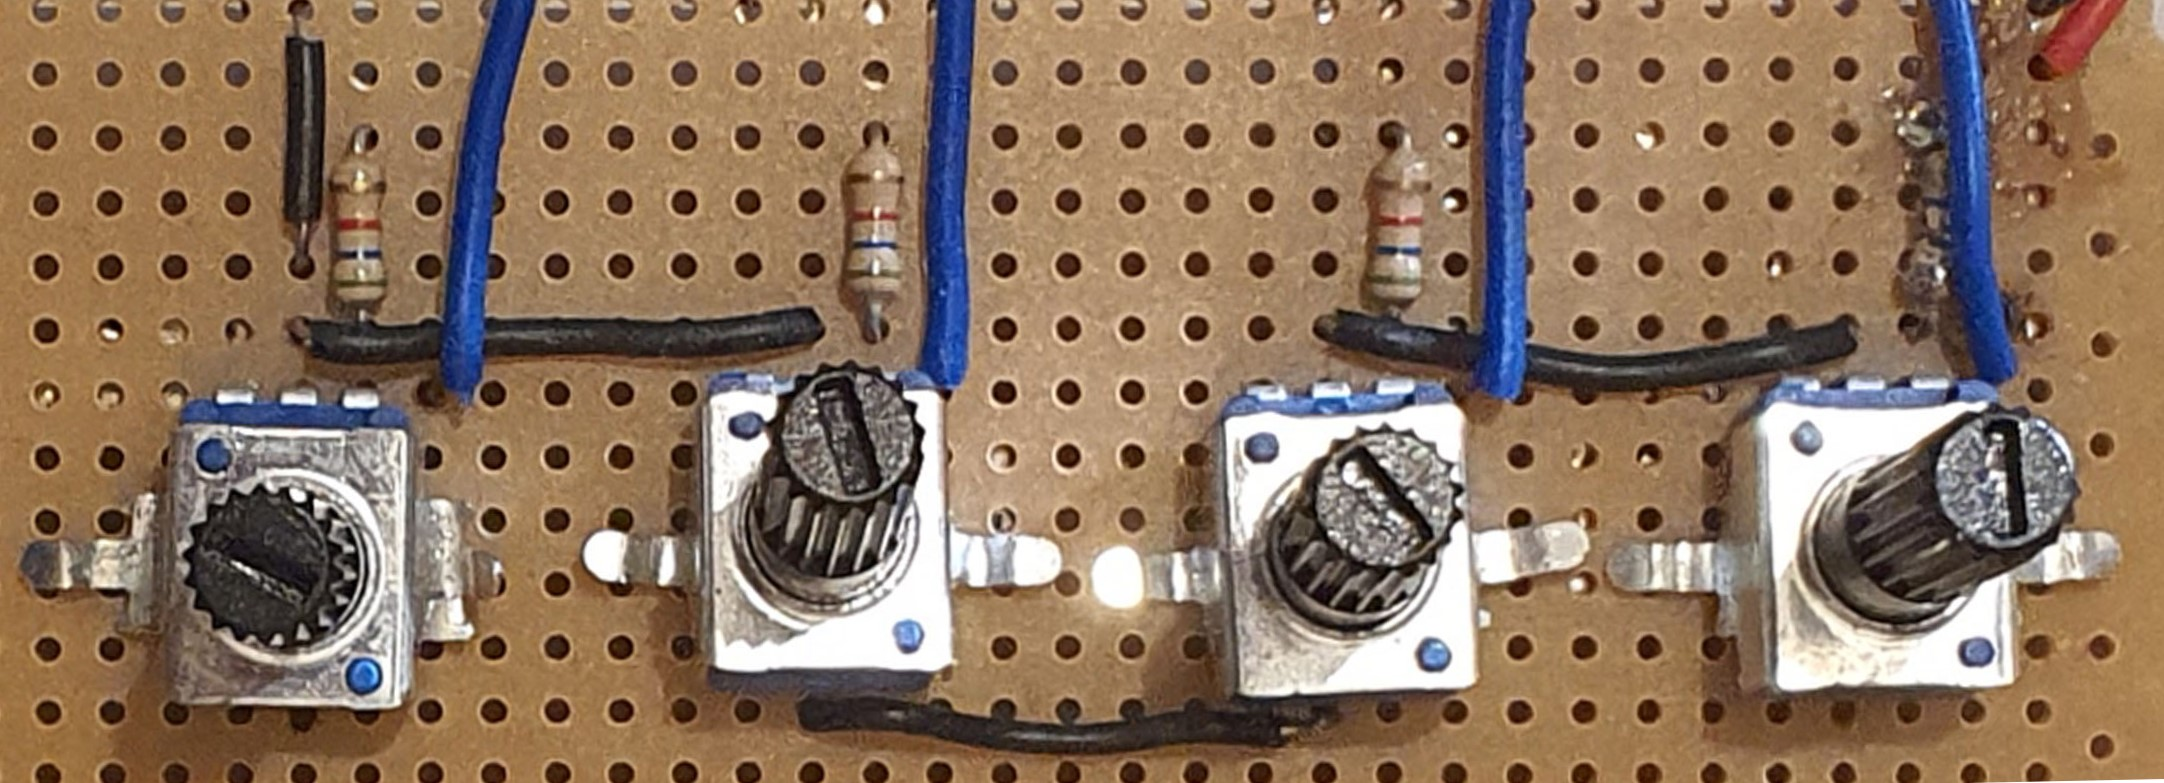
\includegraphics[width=0.6\textwidth]{./images/sensors_circuit.jpg}
		\caption{Protoboard amb el circuit}
		\label{protoboard}
	\end{center}
\end{figure}

\subsection{Desenvolupament i implementació del codi}

Tal com s'ha comentat anteriorment la PCB que s'està utilitzant conté un ADC de dotze canals que s'utilitza per llegir valors de voltatge.

%Importar adcsinglechannel
En aquest exemple, l'objectiu és aconseguir la lectura dels valors del voltatge d'un pin de la PCB.
El següent codi permet fer una mesura del canal que s'indiqui a través de l'argument.
Inicialitza l'ADC de la PCB, pren le mesura i posteriorment retorna el resultat en mil·livolts.

\begin{lstlisting}[language=C]
static uint16_t takeMeasurement(uint_least8_t adcIndex){
	ADC_Handle adc;
	ADC_Params params;
	ADC_init();
	ADC_Params_init(&params);
	adc = ADC_open(adcIndex, &params);
	if (adc == NULL){
		Log_info0("ADC start Failed");
		while(1);
	}
	int_fast16_t res;
	uint16_t adcValue;
	res = ADC_convert(adc, &adcValue);
	
	if (res == ADC_STATUS_SUCCESS) {
		Log_info1("ADC result %d mV", adcValue);
	}
	else {
		Log_info0("ADC status failure");
	}
	ADC_close(adc);
	return adcValue;
}
\end{lstlisting}

Finalment, cal canviar el codi de BLE perquè quan es llegeixin els atributs es retorni el valor mesurat a l'ADC.
Per tant cal canviar la funció environmentalService\_ReadAttrCB tal com es veu a continuació.

\begin{lstlisting}[language=C]
  if(!memcmp(pAttr->type.uuid, temperatureUUID, pAttr->type.len))
{
	uint16_t adcValue = takeMeasurement(Board_ADC0);
	*pLen = (uint16_t)temperatureLen;
	memcpy(pValue, &adcValue, *pLen);
}
else if(!memcmp(pAttr->type.uuid, humidityUUID, pAttr->type.len))
{
	uint16_t adcValue = takeMeasurement(Board_ADC1);
	*pLen = (uint16_t)humidityLen;
	memcpy(pValue, &adcValue, *pLen);
}
\end{lstlisting}



\section{Aplicació mòbil}
Per veure un exemple simplificat d'un client que consumís els serveis oferits per la PCB, s'ha realitzat un desenvolupament propi d'una aplicació per a Android.
Aquesta aplicació llegeix contínuament els valors dels quatre atributs que té la PCB que corresponen amb els sensors.

Per poder interactuar amb la PCB el primer que cal és tenir en compte l'adreça del dispositiu i els identificadors, tant del servei, com dels atributs.
Aquests es poden veure a la taula \ref{taula_app}.

\begin{table}[!h]
	\begin{center}
		\begin{tabular}{|c|l|}
			\hline
			Identificador	&	Valor	\\	\hline
			deviceAddress	&	00:81:F9:4A:4D:B3	\\	\hline
			serviceUUID		&	f0001234-0451-4000-b000-00000000		\\	\hline
			temperatureUUID	&	f0002345-0451-4000-b000-000000000000	\\	\hline
			humidityUUID	&	f0003456-0451-4000-b000-000000000000	\\	\hline
			heartRateUUID	&	f0004567-0451-4000-b000-000000000000	\\	\hline
			bloodOxygenUUID	&	f0005678-0451-4000-b000-000000000000	\\	\hline
		\end{tabular}
		\label{taula_app}
	\end{center}
	\caption{Tipus d'anunciaments}
\end{table}

Per realitzar l'aplicació d'Android cal declarar que requereix els permisos de Bluetooth i específicament de Bluetooth Low Energy.

\begin{lstlisting}[language=xml]
	<uses-permission android:name="android.permission.BLUETOOTH"/>
	<uses-feature android:name="android.hardware.bluetooth_le" android:required="true"/>
\end{lstlisting}

Per implementar el BLE en Android s'ha utilitzat la llibreria nativa que es pot trobar a \cite{ble_library} i s'ha seguit la guia que es troba a \cite{ble_overview}.

Primerament, per poder utilitzar BLE, s'inicialitza l'adaptador corresponent.

\begin{lstlisting}[language=java]
final BluetoothManager bluetoothManager =
	(BluetoothManager) getSystemService(Context.BLUETOOTH_SERVICE);
BluetoothAdapter bluetoothAdapter = bluetoothManager.getAdapter();
\end{lstlisting}

A continuació es comença a escanejar per buscar dispositius.
Per fer-ho es defineix una funció de \textit{callback} que filtrarà els dispositius per comprovar que es troba el que es vol.

\begin{lstlisting}[language=java]
bluetoothLeScanner.startScan(leScanCallback);
\end{lstlisting}

La funció leScanCallback quan trobi el dispositiu al qual vol connectar-se, deixarà d'escanejar i procedirà a intentar connectar-s'hi.
\begin{lstlisting}[language=java]
if(result.getDevice().getAddress().equals(deviceAddress)){
	bluetoothLeScanner.stopScan(leScanCallback);
	device = result.getDevice();
	bluetoothGatt = device.connectGatt(getApplicationContext(), false, gattCallback);
}
\end{lstlisting}

A l'establir la connexió es descobreixen els serveis del dispositiu.
S'obté el servei específic que volem i es llegeixen les característiques corresponents.

\begin{lstlisting}[language=java]
BluetoothGattService service = gatt.getService(
	UUID.fromString(serviceUUID));
characteristicList = service.getCharacteristics();
readCharacteristic(gatt);
\end{lstlisting}

Per cada característica que es llegeix, per obtenir el seu valor tal com es vol i no com l'envia BLE (en little-endian), cal especificar el format que té.
En aquest cas, com que s'han definit en 2 bytes les longituds de les característiques en la PCB, cal especificar que són nombres enters \textit{unsigned} (sense signe) codificats en 16 bits.

\begin{lstlisting}[language=java]
int characteristicValue = characteristic.getIntValue(
BluetoothGattCharacteristic.FORMAT_UINT16, 0);
\end{lstlisting}

Les dades que s'estan transmetent per cada atribut corresponen al valor del voltatge.
Tot i això, per caracteritzar aquestes dades a l'aplicació s'interpreten com si fossin valors plausibles de les mesures que s'estan prenent.
Igualment, es mostra tant una barra de progrés com el valor real de mil·livolts per cada mesura de la PCB.
Però per poder mostrar aquests valors no es pot fer directament.
El codi de BLE és asíncron i es troba en un fil d'execució (\textit{thread} en anglès) diferent al que controla la interfície d'usuari.
Per poder compartir valors entre threads cal utilitzar un \textit{handler}.

Per passar múltiples valors cal fer-ho de la següent manera.
\begin{lstlisting}[language=java]
Bundle bundle = new Bundle();
bundle.putString("value", Integer.toString(characteristicValue));
bundle.putString("characteristic",characteristic.getUuid().toString());
Message message = new Message();
message.obj = bundle;
updateHandler.sendMessage(message);
\end{lstlisting}

Aquests valors es reben a una funció que ja sí que pot modificar la interfície d'usuari i s'obtenen tal i es mostra en el codi a continuació.

\begin{lstlisting}[language=java]
 Handler updateHandler = new Handler(){
	@Override
	public void handleMessage(@NonNull Message msg) {
		super.handleMessage(msg);
		Bundle data = (Bundle) msg.obj;
		String characteristic = data.getString("characteristic");
		String value = data.getString("value");
		...
	}
}
\end{lstlisting}

Abans de modificar la interfície cal adaptar els valors que es reben per mostrar-los representant els sensors que s'han simulat.
Es suposa que els valors rebuts estaran entre 0 i 3000 que són els milivolts que ha llegit l'ADC de la PCB.
Cada mesura es caracteritza diferent, a continuació es pot observar el cas de la temperatura.

\begin{lstlisting}[language=java]
 switch (characteristic) {
	case temperatureUUID: {
		int val = Integer.parseInt(value);
		int progress = val * 30 / 3000;
		TextView tmpConverted =findViewById(R.id.temperatureConverted_lbl);
		TextView temperatureRaw = findViewById(R.id.temperatureRaw_lbl);
		ProgressBar pb = findViewById(R.id.temperature_pb);
		tmpConverted.setText(progress + "C");
		temperatureRaw.setText(value + "mV");
		pb.setProgress(progress);
		break;
	}
\end{lstlisting}

En aquest cas, la temperatura s'assumeix que tindrà valors des de 0 fins a 30 graus.
Finalment, es calcula el seu valor en graus i es canvia la interfície perquè representi el valor.
El codi complet de l'aplicació que s'ha realitzat es pot trobar a \cite{android_repo}.

\section{Escenari}
Finalment, un cop desenvolupat el circuit per simular sensors, el codi necessari per mostrejar i transmetre els valors i una aplicació per rebre aquests valors, l'escenari és el següent.

El circuit que simula els 4 sensors es connecta als pins de la PCB (veure apèndix \ref{datasheet}) que tenen ADC segons el manual de la PCB que es pot trobar a \cite{manual_placa} seguint la taula \ref{connexions}.

\begin{table}[!h]
	\begin{center}
		\begin{tabular}{|c|c|c|}
			\hline
			ADC			&	DIO		& 	PIN		\\	\hline
			0			&	23		&	2		\\	\hline
			1			&	24		&	6		\\	\hline
			2			&	25		&	23		\\	\hline
			3			&	26		&	24		\\	\hline
		\end{tabular}
	\end{center}
	\caption{Taula dels pins amb ADC}
	\label{connexions}
\end{table}

Les connexions des del circuit fins a la PCB es fan a través dels ports que proporciona la PCB a la seva part de darrere que es veuen a la Figura \ref{ports_placa}.

\begin{figure}[h]
	\begin{center}
		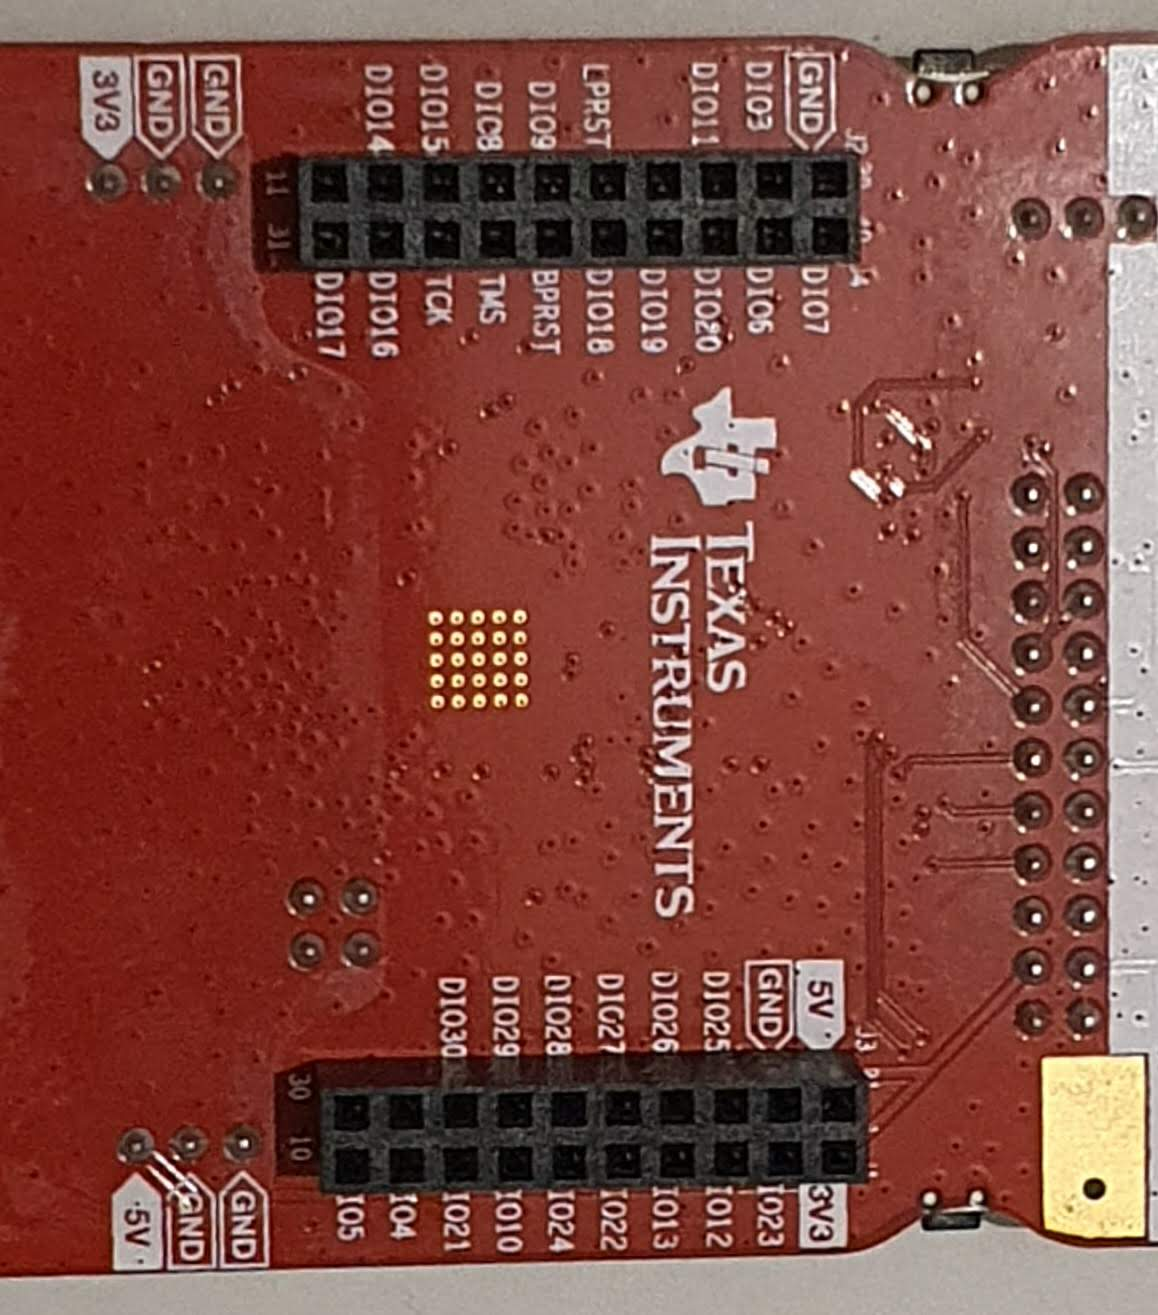
\includegraphics[angle=90, width=0.7\textwidth]{./images/connexions_placa.jpg}
		\caption{Ports de la PCB}
		\label{ports_placa}
	\end{center}
\end{figure}

Un cop fetes les connexions, cal executar el codi de la PCB i clicar el botó d'escanejar de l'aplicació.
Cal tenir en compte que durant el procés d'escaneig, degut a la configuració de BLE, sempre és possible (tot i que poc probable) que el mòbil no descobreixi la PCB un cop transcorregut el temps establert.
En aquest cas, cal tornar a clicar el botó d'escaneig.
Un cop l'aplicació està escanejant es poden canviar les posicions dels potenciòmetres i s'observa com els valors corresponents en el mòbil canvien amb poca latència.
Es pot veure una captura del disseny de l'aplicació a la Figura \ref{captura_app}.

\begin{figure}[h!]
	\begin{center}
		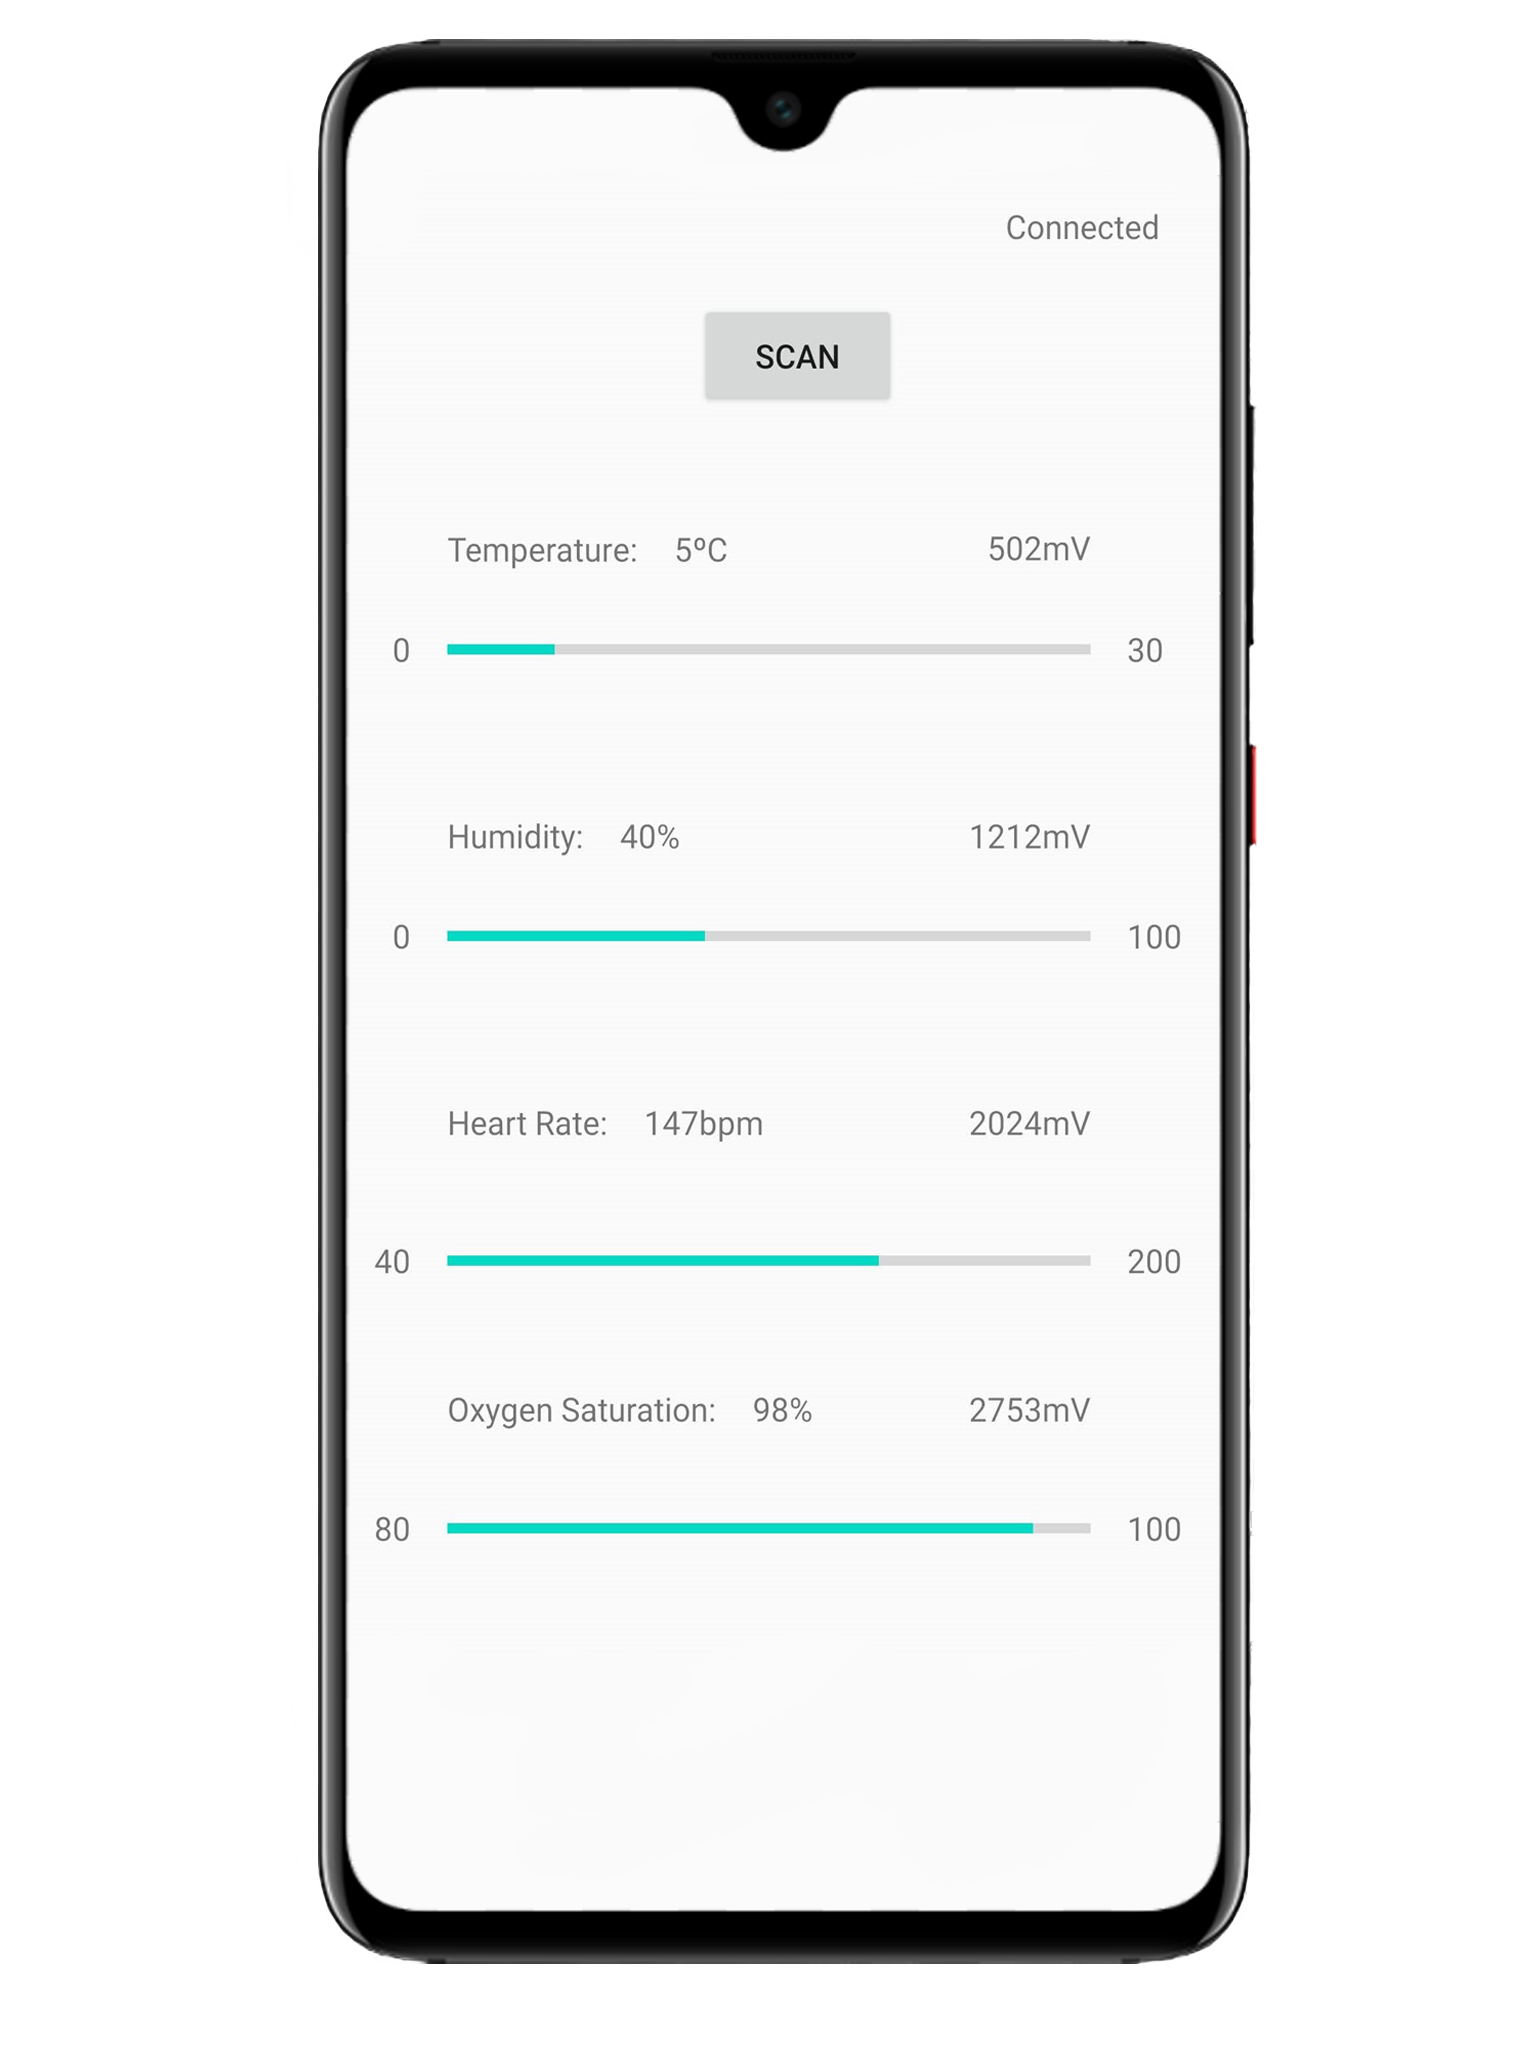
\includegraphics[width=0.6\textwidth]{./images/captura_app_borde.png}
		\caption{Aplicació mòbil}
		\label{captura_app}
	\end{center}
\end{figure}

\section{Continuitat del projecte}
Un cop executat el projecte i entès tant la tecnologia Bluetooth Low Energy com l'entorn de desenvolupament, hi ha aspectes en els quals és possible profunditzar més.
Aquestes es podrien tractar en un altre futur treball.

Tal com s'ha esmentat quan s'ha realitzat l'estudi del consum d'energia utilitzant Energy Trace, els valors obtinguts no es poden considerar absoluts.
És per això que, per poder determinar el temps de vida amb diferents configuracions del BLE s'hauria de mesurar el consum amb un oscil·loscopi mentre la PCB està configurada amb la font d'alimentació externa.

La implementació pràctica de BLE que s'ha realitzat no utilitza cap servei propietari.
Seria interessant implementar un servei estandarditzat i tenir algun dispositiu comercial que pogués connectar-se a la PCB.

Finalment, tot i haver-se desenvolupats projectes que permeten mesurar els voltatges dels ADC i emetre notificacions, per part de BLE, no s'ha aconseguit que sigui alhora.


\cleardoublepage
\phantomsection
\chapter*{Conclusions}

Aquest projecte serveix per considerar si BLE és la tecnologia adequada per a les aplicacions de mesures mediambientals o biològiques.

%\section*{Taxa de dades necessària}

%Un dels dubtes a l'inici del treball era si aquesta tecnologia tenia una capacitat de transmissió suficient per a xarxes de sensors.
%Tot i que el Bluetooth Low Energy té bastant menys capacitat per transmetre dades comparant amb tecnologies com wifi, les dades necessàries en aquest tipus de xarxes acostumen a ser molt reduïdes.
%La tecnologia BLE no és capaç de transmetre vídeo o àudio en temps real però és suficient per transmetre fluxos de dades de sensors amb mesures biològiques o mediambientals.

\section*{Abast}

Com s'ha comentat, l'abast de la tecnologia BLE ve limitat tant per la distància entre transmissor i receptor com per les interferències.
En mesures biològiques es pot considerar que el transmissor i el receptor estaran relativament a prop, per tant, no hi haurà problemes d'abast.
En canvi, per a mesures ambientals si considerem instal·lacions privades en habitatges, cal tenir en compte els obstacles que s'oposen al senyal.
També cal considerar la interferència més que probable de les tecnologies amb les quals BLE comparteix espectre com wifi, altres dispositius intel·ligents o amb Bluetooth Clàssic mateix.
Per combatre aquests desavantatges BLE té múltiples estratègies.
Primerament, sempre és possible augmentar la potència de transmissió (fins al límit permès), però reduint el cicle de vida de la bateria.
També es poden utilitzar capes físiques que implementen més redundància (\textit{LE Coded}).
Finalment, BLE implementa salts en freqüència i la \textit{Slot Availability Mask} per combatre interferències.

Totes aquestes tècniques augmenten la complexitat del protocol però ajuden a poder tenir un gran abast.
A més a més, BLE utilitza canals de freqüència estrets comparats amb altres tecnologies com wifi per tant, les interferències afecten menys a BLE que a altres tecnologies amb canals més amples.

\section*{Consum d'Energia}

BLE és dels protocols que permet consumir menys energia per a transmetre informació.
Això només serà un avantatge quan els sensors estiguin alimentats per bateria i la transmissió sigui el que consumeix més energia de tot el sistema.
Si els sensors tenen pantalles, s'alimenten de la instal·lació elèctrica, fan un processament de les dades o emmagatzemen les dades localment; és possible que el consum de la transmissió no sigui significant.
En aquests casos no s'ha d'escollir el protocol de transmissió segons el consum, ja que el temps entre recàrregues no es veu especialment afectat pel protocol.

En els escenaris on és important tenir un consum baix d'energia, el protocol BLE és una molt bona opció.
Com ja s'ha comentat múltiples vegades, BLE defineix moltes opcions d'implementació i això suposa una flexibilitat molt important.
Aquesta flexibilitat permet, per exemple, poder prescindir de les transmissions redundants com el reconeixement.
Tanmateix, es pot utilitzar la latència d'esclau per reduir els esdeveniments d'una connexió quan no són necessaris.
També, permet transmetre molta informació sense necessitat d'establir una connexió.

Així doncs, poder evitar realitzar tots aquests procediments permet reduir significativament el consum que suposa la transmissió de dades i fa possible augmentar el cicle de vida de la bateria o reduir la mida d'aquesta.
Gràcies a BLE és possible que dispositius no hagin d'estar connectats a cap altre dispositiu a través de cables ni a la xarxa elèctrica.

\section*{Penetració del mercat}

Quan en un projecte hi ha usuaris involucrats d'alguna manera, és molt probable que el telèfon mòbil sigui un component important.
BLE té el gran avantatge que ve incorporat en tots els mòbils intel·ligents.
Això facilita l'ús, ja que els usuaris estan més acostumats, i simplifica l'arquitectura d'un desplegament.
L'arquitectura és més simple perquè el mateix dispositiu mòbil és el receptor de les dades.
En cas de no utilitzar BLE, no hi ha cap tecnologia de baix consum que es pugui connectar directament amb els telèfons dels usuaris.
Altres tecnologies acostumen a utilitzar un dispositiu entre els sensors i els usuaris que s'anomena concentrador o \textit{hub}.
A l'afegir un nou dispositiu s'incrementa el cost d'un desplegament.
A més a més, augmenta la complexitat del flux de dades i també incrementa l'ús de la banda freqüencial, ja que calen més transmissions per la mateixa quantitat d'informació.

En canvi, en el cas de connexió directa fins al terminal de l'usuari BLE és perfecte.
No només està present en telèfons mòbils sinó també en: joguines, televisors, electrodomèstics, càmeres, comandaments a distància, entre d'altres...
En total es preveu la producció de 7.500 milions de dispositius entre 2020 i 2024 amb un creixement del 26\% anual segons el SIG \cite{Bluetooth_Market_Update_2020}.


\cleardoublepage
\phantomsection
\begin{thebibliography}{2}

\bibitem{Bluetooth Specification}
Bluetooth Special Interest Group
``Bluetooth Core Specification``
(Revision 5.2)

\bibitem{Diccionari_Telecomunicacions}
UNIVERSITAT POLITÈCNICA DE CATALUNYA; TERMCAT, CENTRE DE TERMINOLOGIA; ENCICLOPÈDIA CATALANA. Diccionari de telecomunicacions [en línia]. Barcelona: TERMCAT, Centre de Terminologia, cop. 2017. (Diccionaris en Línia) (Ciència i Tecnologia)
\href{https://www.termcat.cat/ca/diccionaris-en-linia/235}{https://www.termcat.cat/ca/diccionaris-en-linia/235}

\bibitem{Original_BLE_Extension}
Honkanen, M.; Lappetelainen, A.; Kivekas, K. (2004). \textit{Low end extension for Bluetooth}. 2004 IEEE Radio and Wireless Conference 19–22 September 2004. IEEE. pp. 199–202.
[Consulta: Octubre 2020] \href{https://ieeexplore.ieee.org/document/1389107}{https://ieeexplore.ieee.org/document/1389107}

\bibitem{MIMOSA}
Arxiu del lloc web de MIMOSA. [Consulta: Octubre 2020]\newline
\href{https://web.archive.org/web/20160804035320/http://www.mimosa-fp6.com/}{https://web.archive.org/web/20160804035320/http://www.mimosa-fp6.com/}

\bibitem{manets}
La informació de la taula s'ha obtingut dels següents enllaços:
\href{https://en.wikipedia.org/wiki/Bluetooth_Low_Energy}{https://en.wikipedia.org/wiki/Bluetooth\_Low\_Energy}
\newline
\href{https://zigbeealliance.org/zigbee-faq}{https://zigbeealliance.org/zigbee-faq}
\newline
\href{https://en.wikipedia.org/wiki/Z-Wave}{https://en.wikipedia.org/wiki/Z-Wave}
\newline
\href{https://en.wikipedia.org/wiki/Insteon}{https://en.wikipedia.org/wiki/Insteon}
\newline
\href{https://en.wikipedia.org/wiki/LoRa}{https://en.wikipedia.org/wiki/LoRa}

\bibitem{BLE_5_improvement_over_4}
Millores de BLE 5 respecte BLE 4. [Consulta: Octubre 2020]\newline
\href{https://www.bluetooth.com/wp-content/uploads/2019/03/Bluetooth\_5-FINAL.pdf}{https://www.bluetooth.com/wp-content/uploads/2019/03/Bluetooth\_5-FINAL.pdf}

\bibitem{ble_feq}
Figura basada de la que es troba a [Consulta: Octubre 2020]:\newline \href{https://microchipdeveloper.com/wireless:ble-phy-layer}{https://microchipdeveloper.com/wireless:ble-phy-layer} 

\bibitem{LoRaWan_Energy}
Casals Ibáñez, Lluis \& Mir Masnou, Bernat \& Vidal Ferré, Rafael \& Gomez, Carles. (2017). \textit{Modeling the energy performance of LoRaWAN}. Sensors. 17. 2364. 10.3390/s17102364. 
[Consulta: Octubre 2020] \newline
\href{https://www.researchgate.net/publication/320435869}{https://www.researchgate.net/publication/320435869}

\bibitem{802.15.4_throughput}
Latré, Benoît; De Mil, Pieter; Moerman, Ingrid; Dierdonck, Niek; Dhoedt, Bart; Demeester, Piet. (2005).
[Consulta: Octubre 2020] \href{https://www.researchgate.net/publication/220963645_Maximum_Throughput_and_Minimum_Delay_in_IEEE_802154}{Maximum Throughput and Minimum Delay in IEEE 802.15.4.} 3794. 866-876. 10.1007/11599463\_84.

\bibitem{BLE_Review}
Gomez, C.; Oller, J.; Paradells, J.  \href{https://www.mdpi.com/1424-8220/12/9/11734}{Overview and Evaluation of Bluetooth Low Energy: An Emerging Low-Power Wireless Technology}. Sensors 2012, 12, 11734-11753.
[Consulta: Octubre 2020]

\bibitem{Link_Layer_states}
Link Layer States [Consulta: Octubre 2020]\newline
\href{https://dev.ti.com/tirex/explore/content/simplelink_academy_cc13x2_26x2sdk_4_10_01_00/modules/ble5stack/ble_connections/ble_connections.html\#the-link-layer}{https://dev.ti.com/tirex/explore/content/simplelink\_academy\_cc13x2\_26x2sdk\_4\_10\_01\_00/modules/ble5stack/ble\_connections/ble\_connections.html\#the-link-layer}

\bibitem{ble_stack}
Figura basada de la que es troba a [Consulta: Octubre 2020]:\newline
\href{http://software-dl.ti.com/lprf/simplelink_cc2640r2_sdk/1.00.00.22/exports/docs/blestack/html/ble-stack/index.html}{http://software-dl.ti.com/lprf/simplelink\_cc2640r2\_sdk/1.00.00.22/exports/docs/blestack/html/ble-stack/index.html}

\bibitem{services}
Bluetooth Special Interest Group
``GATT Services Specification``
[Consulta: Octubre 2020]\newline
\href{https://www.bluetooth.com/specifications/gatt/services/}{https://www.bluetooth.com/specifications/gatt/services/}

\bibitem{characteristics}
Bluetooth Special Interest Group ``GATT Charasteristics Specification``\newline
[Consulta: Octubre 2020]\newline
\href{https://www.bluetooth.com/specifications/gatt/characteristics/}{https://www.bluetooth.com/specifications/gatt/characteristics/}

\bibitem{GATT_Hierarchy}
O’Reilly online learning
Chapter 4. GATT (Services and Characteristics) \newline
[Consulta: Octubre 2020] \newline
\href{https://www.oreilly.com/library/view/getting-started-with/9781491900550/ch04.html}{https://www.oreilly.com/library/view/getting-started-with/9781491900550/ch04.html}

\bibitem{Battery_Level}
Especificació de la característica de nivell de bateria.\newline
[Consulta: Octubre 2020]\newline
\href{https://www.bluetooth.com/wp-content/uploads/Sitecore-Media-Library/Gatt/Xml/Characteristics/org.bluetooth.characteristic.battery\_level.xml}{https://www.bluetooth.com/wp-content/uploads/Sitecore-Media-Library/Gatt/Xml/Characteristics/org.bluetooth.characteristic.battery\_level.xml}

\bibitem{Temperature_Characteristic}
Especificació de la característica de temperatura.
[Consulta: Octubre 2020] \newline
\href{https://www.bluetooth.com/wp-content/uploads/Sitecore-Media-Library/Gatt/Xml/Characteristics/org.bluetooth.characteristic.temperature.xml}{https://www.bluetooth.com/wp-content/uploads/Sitecore-Media-Library/Gatt/Xml/Characteristics/org.bluetooth.characteristic.temperature.xml}

\bibitem{reservedUUIDs}
Llistat de UUID reservats per a empreses.
[Consulta: Octubre 2020]\newline
\href{https://www.bluetooth.com/specifications/assigned-numbers/}{https://www.bluetooth.com/specifications/assigned-numbers/}

\bibitem{descriptors}
Bluetooth Special Interest Group
``GATT Descriptors Specification``
[Consulta: Octubre 2020]\newline
\href{https://www.bluetooth.com/specifications/gatt/descriptors/}{https://www.bluetooth.com/specifications/gatt/descriptors/}

\bibitem{Advertising}
Blog oficial sobre els anuncis en BLE. [Consulta: Octubre 2020]\newline
\href{https://www.bluetooth.com/blog/bluetooth-low-energy-it-starts-with-advertising/}{ https://www.bluetooth.com/blog/bluetooth-low-energy-it-starts-with-advertising/}

\bibitem{adv_ext}
Figura basada de la que es troba a [Consulta: Octubre 2020]:\newline
\href{https://www.nordicsemi.com/Products/Low-power-short-range-wireless/Bluetooth-5}{https://www.nordicsemi.com/Products/Low-power-short-range-wireless/Bluetooth-5}

\bibitem{advertisment_params}
Diagrama dels paràmetres d'anunci.
[Consulta: Octubre 2020] \newline
\href{https://dev.ti.com/tirex/explore/content/simplelink\_academy\_cc13x2\_26x2sdk\_4\_10\_01\_00/modules/ble5stack/ble\_scan\_adv\_basic/ble\_scan\_adv\_basic.html}{https://dev.ti.com/tirex/explore/content/simplelink\_academy\_cc13x2\_26x2sdk\_4\_10\_01\_00/modules/ble5stack/ble\_scan\_adv\_basic/ble\_scan\_adv\_basic.html}

\bibitem{fig:connection_establishement}
Diagrama del procés de connexió.
[Consulta: Octubre 2020] \newline
\href{https://microchipdeveloper.com/wireless:ble-link-layer-connections}{https://microchipdeveloper.com/wireless:ble-link-layer-connections}

\bibitem{slave_latency}
Diagrama de la latència d'esclau.
[Consulta: Octubre 2020] \newline
\href{http://software-dl.ti.com/lprf/simplelink\_cc2640r2\_latest/docs/blestack/ble\_user\_guide/html/ble-stack-3.x/gap.html\#connection-parameters}{http://software-dl.ti.com/lprf/simplelink\_cc2640r2\_latest/docs/blestack/ble\_user\_guide/html/ble-stack-3.x/gap.html\#connection-parameters}

\bibitem{BLE_4.2_packet_format}
BLUETOOTH SPECIFICATION Version 4.2 [Vol 6, Part B] apartat 2 \newline
[Consulta: Octubre 2020]

\bibitem{AD_Types}
Estructures de les dades d'anunci possibles\newline
[Consulta: Octubre 2020] \newline
\href{https://www.bluetooth.com/specifications/assigned-numbers/generic-access-profile/}{https://www.bluetooth.com/specifications/assigned-numbers/generic-access-profile/}

\bibitem{BLE_5_Extended_Advertising}
BLUETOOTH CORE SPECIFICATION Version 5.2 | Vol 6, Part B apartat 2.3.4

\bibitem{Mesh Profile Definition}
\href{https://www.bluetooth.org/docman/handlers/downloaddoc.ashx?doc_id=429633}{https://www.bluetooth.org/docman/handlers/downloaddoc.ashx?doc\_id=429633}

\bibitem{Mesh Profile Models}
\href{https://www.bluetooth.org/docman/handlers/downloaddoc.ashx?doc_id=429634}{https://www.bluetooth.org/docman/handlers/downloaddoc.ashx?doc\_id=429634}


\bibitem{Mesh Profile}
\href{https://www.techbriefs.com/component/content/article/tb/supplements/st/features/articles/33885}{https://www.techbriefs.com/component/content/article/tb/supplements/st/features/articles/33885}

\bibitem{Mesh Profile Overview}
\href{https://www.bluetooth.com/wp-content/uploads/2019/03/Mesh-Technology-Overview.pdf}{https://www.bluetooth.com/wp-content/uploads/2019/03/Mesh-Technology-Overview.pdf}

\bibitem{placa}
Fotografia del LaunchXL CC1352R
[Consulta: Octubre 2020]\newline
\href{http://www.ti.com/diagrams/med_launchxl-cc1352r1_launchxl-cc1352r1.jpg}{http://www.ti.com/diagrams/med\_launchxl-cc1352r1\_launchxl-cc1352r1.jpg}

\bibitem{placa_datasheet}
CC1352R SimpleLink Datasheet
[Consulta: Octubre 2020]\newline
\href{https://www.ti.com/tool/LAUNCHXL-CC1352R1\#technicaldocuments}{https://www.ti.com/tool/LAUNCHXL-CC1352R1\#technicaldocuments}

\bibitem{eclipse}
Web de l'entorn de desenvolupament Eclipse.
[Consulta: Octubre 2020] \newline
\href{https://www.eclipse.org/ide/}{https://www.eclipse.org/ide/}

\bibitem{project0_UUIDs}
Figura dels UUID del Project 0 [Consulta: Octubre 2020]\newline
\href{https://dev.ti.com/tirex/explore/content/simplelink_academy_cc13x2_26x2sdk_4_20_00_00/modules/ble5stack/ble_01_basic/ble_01_basic.html}{https://dev.ti.com/tirex/explore/content/simplelink\_academy\_cc13x2\_26x2sdk\_4\_20\_00\_00/modules/ble5stack/ble\_01\_basic/ble\_01\_basic.html}


\bibitem{extended properties}
Characteristic Extended Properties
[Consulta: Octubre 2020]\newline
\href{https://www.bluetooth.com/wp-content/uploads/Sitecore-Media-Library/Gatt/Xml/Descriptors/org.bluetooth.descriptor.gatt.characteristic_extended_properties.xml}{https://www.bluetooth.com/wp-content/uploads/Sitecore-Media-Library/Gatt/Xml/Descriptors/org.bluetooth.descriptor.gatt.characteristic\_extended\_properties.xml}

\bibitem{serial_params}
Configuració del port sèrie
[Consulta: Octubre 2020] \newline
\href{http://dev.ti.com/tirex/explore/content/simplelink_academy_cc13x2_26x2sdk_4_10_01_00/modules/ble5stack/ble_01\_basic/resources/btool_serial_port_config.png}{http://dev.ti.com/tirex/explore/content/simplelink\_academy\_cc13x2\_26x2sdk\_4\_10\_01\_00/modules/ble5stack/ble\_01\_basic/resources/btool\_serial\_port\_config.png}

\bibitem{Service_Generator}
Generador de fitxers per a nous serveis 
[Consulta: Octubre 2020] \newline
\href{http://dev.ti.com/tirex/explore/content/simplelink\_academy\_cc13x2\_26x2sdk\_4\_10\_01\_00/modules/ble5stack/ble\_01\_custom\_profile/ble\_01\_custom\_profile.html\#example-service-generator}{http://dev.ti.com/tirex/explore/content/simplelink\_academy\_cc13x2\_26x2sdk\_4\_10\_01\_00/modules/ble5stack/ble\_01\_custom\_profile/ble\_01\_custom\_profile.html\#example-service-generator}

\bibitem{ble_library}
\href{https://developer.android.com/reference/android/bluetooth/le/package-summary}{https://developer.android.com/reference/android/bluetooth/le/package-summary}


\bibitem{ble_overview}
\href{https://developer.android.com/guide/topics/connectivity/bluetooth-le}{https://developer.android.com/guide/topics/connectivity/bluetooth-le}

\bibitem{android_repo}
Respositori amb l'aplicació Android desenvolupada. \newline
\href{https://github.com/garretaserra/sensorReader}{https://github.com/garretaserra/sensorReader}

\bibitem{manual_placa}
Manual del LaunchPad CC1352R
[Consulta: Octubre 2020] \newline
\href{https://www.ti.com/lit/pdf/swru525}{https://www.ti.com/lit/pdf/swru525}

\bibitem{Bluetooth_Market_Update_2020}
Anàlisi del mercat de Bluetooth
[Consulta: Octubre 2020] \newline
\href{https://www.bluetooth.com/wp-content/uploads/2020/03/2020\_Market\_Update-EN.pdf}{https://www.bluetooth.com/wp-content/uploads/2020/03/2020\_Market\_Update-EN.pdf}

\end{thebibliography}

%%%%%%%%%%%%%%%%%%%%%%%%%%%%%%%%%%%%%%%%%%%%%%%%%%%%%%%%%%%%%%%%%%%%%%%%%%
%%%%%%                           APENDIXS                         %%%%%%%%
%%%%%%%%%%%%%%%%%%%%%%%%%%%%%%%%%%%%%%%%%%%%%%%%%%%%%%%%%%%%%%%%%%%%%%%%%%
\pagestyle{empty}  % no tocar
 
%% Descomentar una de les dues línies següents, en funció de:
%%  a) els apendixs s'encuadernaran apart (amb portada) 
%%  b) els apendixs s'enquadernen amb el mateix projecte (sense portada). 
%% Recordeu que si tot el document (amb apèndixs) excedeix les 100 pagines 
%% s'ha d'enquadernar a part
%\appendix\ambportada
\appendix\senseportada


%%%%%%%%%%%%%%%%%%%%%%%%%%%%%%%%%%%%%%%%%%%%%%%%%%%%%%%%%%%%%%%%%%%%%%%%%%
%%%%%% INCLOURE A PARTIR D'AQUI TOTS ELS CAPÍTOLS DELS APENDIXS   %%%%%%%%
%%%%%%%%%%%%%%%%%%%%%%%%%%%%%%%%%%%%%%%%%%%%%%%%%%%%%%%%%%%%%%%%%%%%%%%%%%




\chapter{Taula de atributs del Project 0}

\begin{table}[h!]
	\begin{center}
		\tiny
		\csvautotabular{data_files/projectzeroUUID.csv}
	\end{center}
\end{table}



\end{document}






